\documentclass[a4paper]{extarticle}
\usepackage[utf8]{inputenc}
\usepackage[italian]{babel}
\selectlanguage{italian}
\usepackage[table]{xcolor}
\usepackage{xcolor}
\usepackage{circuitikz}
\usepackage{bm}
\usetikzlibrary{patterns,snakes}
\usetikzlibrary{decorations.markings,intersections,calc}
\usepackage{ifthen}
\usetikzlibrary{calc,patterns,angles,quotes}
\usetikzlibrary{positioning, circuits.logic.US}
\usetikzlibrary {shapes.gates.logic.US, shapes.gates.logic.IEC, calc}
\tikzset {branch/.style={fill, shape = circle, minimum size = 3pt, inner sep = 0pt}}
\usetikzlibrary{matrix,calc}
\usetikzlibrary{arrows.meta}
\usetikzlibrary{decorations.markings}
\usetikzlibrary{shapes.geometric}
\usepackage{multirow}
\usepackage{float}
\usepackage{geometry}
\usepackage{pgfplots}
\usepackage{tabularx}
\usepackage{pgf-pie}
\usepackage{tikz}
\usepackage{tikz-3dplot}
\usepackage{amsmath}
\usepackage{amssymb}
\usepackage{color, soul}
\usepackage{fancyhdr}
\usepackage{graphicx}
\usepackage{subfig}
\usepackage{physics}
%\usepackage{luamplib}
%\usepackage{mathdesign}
\usepackage[outline]{contour} % glow around text
\contourlength{1.0pt}
\graphicspath{ {./img/} }
\newtheorem{theorem}{Teorema}[section]
\newtheorem{corollary}{Corollario}[theorem]
\newtheorem{lemma}[theorem]{Lemma}

% Specifiche
\geometry{
 a4paper,
 top=20mm,
 left=30mm,
 right=30mm,
 bottom=30mm
}

\pagestyle{fancy}
\fancyhf{}
\fancyhead[LO]{\nouppercase{\leftmark}}
\fancyfoot[CE, CO]{\thepage}
\addtolength{\headheight}{1em}
\addtolength{\footskip}{-0.5em}

\newcommand{\quotes}[1]{``#1''}
\renewcommand\tabularxcolumn[1]{>{\vspace{\fill}}m{#1}<{\vspace{\fill}}}
\renewcommand\arraystretch{}
\newcolumntype{P}{>{\centering\arraybackslash}X}
\newcommand{\gear}[5]{%
    \foreach \i in {1,...,#1}
    {   [rotate=(\i-1)360/#1] (0:#2) arc (0:#4:#2) {[rounded corners=0.5pt] -- (#4+#5:#3)  arc (#4+#5:360/#1-#5:#3)} --  (360/#1:#2)
    }
}
\newcommand\dif{\mathop{}\!\mathrm{d}}

\title{\textbf{Università di Trieste\\ \vspace{1em}
Laurea in ingegneria elettronica e informatica}}
\author{Enrico Piccin - Corso di Fisica generale II - Prof. Pierluigi Monaco e Prof. Gabriele Cescutti}
\date{Anno Accademico 2022/2023 - 3 Ottobre 2022}

\begin{document}

\vspace{-10mm}
\noindent
\maketitle

\tableofcontents
\newpage

\noindent
\begin{center}
  3 Ottobre 2022
\end{center}

\section{Introduzione all'elettrostatica}
Quando consideriamo una barretta di vetro appesa ad un filo che viene strofinata su un pezzo di lana e la si avvicina ad un'altra barretta, in posizione fissa, la prima si allontana.\\
Se al posto di barrette di vetro si considerano barrette di plastica, si osserva il medesimo fenomeno di allontanamento.\\
Se, però, si considera una barretta di vetro e una di plastica, allora si ottiene un fenomeno opposto: le bacchette si avvicinano.\\
Ciò che, infatti, risulta fondamentale da capire in elettrostatica, è che la forza elettrostatica è sia \textbf{attrattiva} che \textbf{repulsiva}, a seconda della tipologia di cariche elettroniche che interagiscono.\\
Da notare, inoltre, che quando si parla di bacchette di carica positiva o negativa, si sta parlando di bacchette alle quali si sottraggono \textbf{cariche negative} oppure se ne aggiungono, in quanto gli elettroni sono le uniche particelle che si muovono.
La carica dell'elettrone è la seguente
\[\boxed{e = 1.602176634 \times 10^{-19} \text{ C}}\]
Si sta parlando, comunque, di cariche che orbitano attorno al nucleo (il quale presenta un diametro di $5.0 \times 10^{-15} \text{ m}$), mentre il diametro dell'atomo è di circa $2.0 \times 10^{-10} \text{ m}$.

\vspace{1em}
\noindent
\textbf{Osservazione}: Il fatto che gli elettroni non cadano dentro il nucleo, che presenta particelle positive come i protoni, è dettato dal principio di indeterminazione di Heisenberg, il quale afferma che, dal punto di vista quantistico, è impossibile conoscere simultaneamente con precisione sia il momento sia la posizione di una particella.

\vspace{1em}
\subsection{Conduttore}
Si consideri una sfera conduttrice in cui vi sono elettroni che tendono a distribuirsi su un lato della superficie della sfera, lasciando dall'altro lato una carica positiva.
Se a tale sfera viene collegato un cavo conduttore, gli elettroni tenderanno a percorrere tale cavo, diminuendo, di fatto, la quantità di carica negativa presente nella sfera conduttrice.

\vspace{1em}
\noindent
\textbf{Osservazione}: Come si è detto, la carica è quantizzata, e la \textbf{carica base} di un elettrone è
\[\boxed{e = 1.6 \times 10^{-19} \text{ C}}\]
che, ovviamente, presenta un segno negativo. Quando un oggetto è carico, significa che vi è uno squilibrio tra il numero degli elettroni e il numero di protoni.
Si potrebbe scrivere che la quantità di carica è data da
\[q= \left(N_p - N_e\right) \cdot e\]
dove $N_e$, $N_p$ rappresentano il numero di elettroni e di protoni.\\
Non solo, ma dato un oggetto, è possibile definire
\begin{itemize}
  \item \textbf{densità lineare di carica}, definita come $\lambda = \frac{q}{L}$;
  \item \textbf{densità superficiale di carica}, definita come $\sigma = \frac{q}{S}$;
  \item \textbf{densità volumetrica di carica}, definita come $\rho = \frac{q}{V}$.
\end{itemize}
In generale, poi, la quantità di carica totale, in elettrostatica, si \textbf{conserva}.

\vspace{1em}
\noindent
\subsection{Legge di Coulomb}
Per misurare la forza di gravità è stata impiegata la \textit{bilancia di torsione}, impiegando la forza elastica per misurare un'ulteriore forza.
Analogamente, ponendo due cariche opposte vicine le une alle altre, si misura l'angolo che viene descritto dalle due cariche nello spazio angolare: in base a tale dato, unito al fatto che è nota la forza di torsione in funzione dell'angolo stesso, si riesce a determinare la \textbf{forza di Coulomb}.
Di qui si ha che
\[\boxed{\vec{F}_{\text{a,b}} = K \cdot \frac{q_\text{A} \cdot q_\text{B}}{r_{\text{a, b}}^2} \cdot \hat{v}_{\text{a,b}}}\]
Naturalmente la forza ha una sua direzione e un suo verso, oltre che modulo, descritto dal versore.
Per la $3^{\circ}$ legge di Newton, si ha naturalmente che
\[\vec{F}_{\text{a,b}} = \vec{F}_{\text{b,a}}\]
ovvero le forze sono opposte a seconda del versore impiegato. Si ha che la costante $\epsilon_0$ è la costante dielettrica del vuoto, definita come
\[\epsilon_0 = 8.854 \times 10^{-12} \text{ } \frac{\text{C}^2}{\text{N} \cdot \text{m}^2}\]
Mentre la costante $K$ di Coulomb è 
\[\boxed{K = \frac{1}{4 \pi \epsilon_0} = 9 \times 10^{9} \text{ } \frac{\text{N} \cdot \text{m}^2}{\text{C}^2}}\]

\vspace{1em}
\noindent
\textbf{Osservazione}: La carica di $1$ C è molto elevata, in quanto se si pongono due cariche da $1$ C a distanza di $1$ m si ottiene una forza di Coulomb pari a $F_{\text{a, b}} = 9 \times 10^9$ N, che è elevatissima.\\
Non solo, si osservi che le forze attrattive agenti su un corpo si sommano, al fine di ottenere la forza risultante.

\vspace{1em}
\noindent
\textbf{Esempio 1}: Per capire se, date due cariche, risulta più significativa la forza di gravità o la forza di Coulomb, è sufficiente considerare due protoni entrambi di carica elementare $e$, posti a distanza $x$.
In particolare is ha che
\begin{itemize}
  \item La forza di Coulomb è data $F_{\text{C}, \text{a, b}} = K \cdot \frac{e^2}{x^2}$
  \item La forza di gravità è data da $F_{\text{G}, \text{a, b}} = G \cdot \frac{m_\text{p}^2}{x^2}$
\end{itemize}
Da cui si evince che il loro rapporto è dato da
\[\frac{F_{\text{C}, \text{a, b}}}{F_{\text{G}, \text{a, b}}} = \frac{e^2}{m_\text{p}^2} \cdot \frac{\text{K}}{\text{G}} = \frac{1.6 \times 10^{-38}}{1.67 \times 10^{-54}} \cdot \frac{9 \times 10^9}{6.67 \times 10^{-11}} = \frac{9}{7} \times 10^{36}\]
il che significa che la forza di Coulomb è circa $10^{36}$ volte quella di gravità.

\vspace{1em}
\noindent
\textbf{Esempio 2}: Due sfere identiche di polistirolo sono appese tramite un filo lungo $l = 30 \times 10^{-2}$ m. Le cariche delle due sfere sono incognite, ma le lor masse, invece, sono $m_1 = m_2 = 0,030 $ kg.
L'angolo descritto dal filo rispetto alla verticale è $\theta = 7^{\circ}$, è facile capire come la distanza delle due cariche sia $30 \times 10^{-2} \text{ m} \cdot \sin(7) \cdot 2 = 39 \times 10^{-2} \text{ m}$.
Non solo, ma è anche noto come
\[m g = T \cos(\theta) \hspace{1em} \text{ e } \hspace{1em} F_\text{C} = T \sin(\theta)\]
per cui si ha che
\[F_\text{C} = mg \tan(\theta)\]
Da ciò si evince come le due cariche siano
\[q_1 = q_2 = \sqrt{\frac{mg \tan(\theta) \cdot (2 l \sin(\theta))^2}{\text{K}}} = 1.46 \times 10^{-7} \text{ C}\]
che si può anche scrivere come $146$ nC.

\newpage
\noindent
\begin{center}
  4 Ottobre 2022
\end{center}
La forza di Coulomb è alla base della forza elettrostatica. Non solo, ma è fondamentale capire che, in elettrostatica, le forze possono essere sia attrattive che repulsive.\\
La carica è quantizzata e le forze elettrostatiche che agiscono su una particella possono essere sommate (secondo le regole del parallelogramma) al fine di determinarne la risultante.

\vspace{1em}
\noindent
\subsection{Campo elettrico}
Esattamente come nel caso del campo gravitazionale, anche il campo elettrico è un campo vettoriale che presenta implicite delle proprietà che attribuisce alle entità che vi interagiscono.\\
Di seguito si espone la definizione di \textbf{campo elettrico}:

% Tabella per le definizione di concetti, etc...
\vspace{1em}
\rowcolors{1}{black!5}{black!5}
\setlength{\tabcolsep}{14pt}
\renewcommand{\arraystretch}{2}
\noindent
\begin{tabularx}{\textwidth}{@{}|P|@{}}
    \hline
    {\textbf{CAMPO ELETTRICO}}\\
    \parbox{\linewidth}{Il campo elettrico, dal punto di vista vettoriale, viene definito come
    \[\vec{E} = \frac{\vec{F}}{q_0}\]
    in cui $q_0$ deve essere piccolo, ed è una carica di prova necessaria per misurare il campo elettrico, in quanto è noto che le cariche fra di loro interagiscono e si influenzano reciprocamente.\\
    Il campo elettrico è additivo, per cui al fine di conoscere il vettore campo elettrico risultante, è sufficiente sommare i vettori campo elettrico secondo la regola del parallelogramma.\vspace{3mm}}\\
    \hline
\end{tabularx}

\vspace{2em}
\noindent
\textbf{Esempio}: Si consideri una carica elettrica piccola $q_0=81 \text{ nC}$ e una forza che agisce su tale carica $\vec{F}$ ..., allora ... continua ...

\vspace{1em}
\noindent
\subsubsection{Campo elettrico generato da una carica puntiforme}
È noto che la forza di Coulomb è data dalla seguente equazione
\[\boxed{\vec F = \frac{1}{4 \pi \epsilon_0} \cdot \frac{q \cdot q_0}{r^2} \cdot \hat{v}}\]
Per cui il campo elettrico generato da una carica puntiforme è dato da
\[\boxed{\vec E = \frac{1}{4 \pi \epsilon_0} \cdot \frac{q}{r^2} \cdot \hat{v}}\]

\vspace{1em}
\noindent
Se ora si dovesse considerare il campo elettrico generato da un insieme di cariche è dato da:
\[\boxed{\vec E = \frac{1}{4 \pi \epsilon_0} \cdot \sum_{i=1}^n \frac{q_i}{r_i^2} \cdot \hat{v_i}}\]

\vspace{1em}
\noindent
\textbf{Esempio}: Data una carica $q=81 \times 10^{-9}$ C ed essendo nota la carica di un elettrone $e = 1.6 \times 10^{-19}$ C, è facile capire che il numero di elettroni persi è dato da:
\[\frac{81 \times 10^{-9}\text{ C}}{1.6 \times 10^{-19}\text{ C}} = 50.6 \times 10^{9}\]

\vspace{1em}
\noindent
\textbf{Osservazione}: In un classico esperimento R.A. Millikan (1868-1953) misure la carica dell'elettrone. L'apparecchiatura the use rappresentata schematicamente nella Figura 1.13. Un nebulizzatore produceva goccioline alcune delle quali cadevano attraverso un foro in una regione in cui era presente un campo elettrico uniform generato da due piatti paralleli carichi. Millikan era in grado di osservare una particolare gocciolina con it microscopio e di determinarne la massa misurandone la velocità limite. Egli caricava poi la gocciolina, irraggiandola con raggi X e regolava it campo elettrico in modo che la goccia rimanesse in equilibria statico sotto 1' azione delle uguali e opposte forze gravitazionale ed elettrica.

\vspace{1em}
\noindent
\subsection{Dipolo elettrico}
Avvicinando un bastoncino carico ad uno non carico, si osserva un avvicinamento dei due oggetti. Il dipolo ha un direzione ben chiara:


% \begin{figure}[H]
%   % DIPOLE - axis beneath
%   \begin{tikzpicture}
%     \def\R{0.48}
%     \def\a{2.0}
%     \def\h{0.7}
%     \coordinate (Q-) at (-\a,\h);
%     \coordinate (Q+) at (+\a,\h);
%     \coordinate (P)  at (+2.5\a,\h);
    
%     \draw[->,thick] (-1.5\a,0) -- (+3.0\a,0);
%     \draw[thick] ( 0,0.15) --++ (0,-0.3) node[below] {0};
%     \draw[thick] (-\a,0.1) --++ (0,-0.2) node[below] {$-a$};
%     \draw[thick] (+\a,0.1) --++ (0,-0.2) node[below] {$+a$};
%     \draw[thick] (2.5\a,0.1) --++ (0,-0.2) node[below] {$x$};
    
%     \draw[vector,line width=2]  (Q-) ++ (\R,0) --++ ({2(\a-\R)},0) node[midway,above] {$\vb{L}$};
%     \draw[charge-] (Q-) circle (\R) node[scale=1.0] {$-q$};
%     \draw[charge+] (Q+) circle (\R) node[scale=1.0] {$+q$};
%     \draw[vector,line width=2,Ecol] (P) --++ (0.9\a,0) node[above=2,above left=0] {$\vb{E}$};
%     \fill (P) circle (0.1) node[above=2] {P}; % node[below=2] {$x$};
%   \end{tikzpicture}
% \end{figure}

\vspace{1em}
\noindent
Allora il momento di dipolo di un dipolo elettrico si calcola come:
\[\vec p = (2aq) \cdot \hat{j}\]
mentre il campo di dipolo si determina come
\[\vec{E}(\vec{r}) = \frac{1}{4 \pi \epsilon_0} \cdot \frac{p}{r^3} \cdot \left[3 \cdot (\hat{r} \cdot \hat{p}) \hat{r} - \hat{p}\right]\]

\vspace{1em}
\noindent
\subsection{Campo elettrico sull'asse di un dipolo}
Un dipolo elettrico è composto da due carica $+q$ e $-q$ separate da una distanza $2a$. Se le due cariche sono posizionate rispettivamente in $(0,0,a)$ e $(0,0,-a)$ sull'asse $z$ (ossia l'asse del dipolo).\\

\vspace{1em}
\noindent
\subsection{Campo elettrico nel piano equatoriale di un dipolo}
Si consideri il campo elettrico in un punto $P$ posto sull'asse $y$. I due contributi di campo sono $\vec{E}_+$, dovuto alla carica positiva, ed $\vec{E}_-$, dovuto alla carica negativa:
\[\vec{E}_+ = \frac{1}{4 \pi \epsilon_0} \cdot \frac{q}{r_+^2} \hat{r}_+ \hspace{1em} \text{ e } \hspace{1em} \vec{E}_- = \frac{1}{4 \pi \epsilon_0} \cdot \frac{-q}{r_-^2} \hat{r}_-\]
La distanza $r_+$ tra $+q$ e $P$ è uguale alla distanza $r_-$ tra $-q$ e $P$ ed è $r_+ = r_- = r = \sqrt{y^2+a^2}$. Com'è evidente, il vettore $\vec{r}_+ = y \hat{j} - a \hat{k}$, per cui il versore $\hat{r}_+$ è la normalizzazione del vettore $\vec{r}_+$ è
\[\hat{r}_+=\frac{y \hat{j} - a \hat{k}}{r}\]
per cui si ottiene
\[\vec{E}_+=\frac{1}{4 \pi \epsilon_0} \frac{q}{r^2} = \frac{y \hat{j} - a \hat{k}}{r} = \frac{1}{4 \pi \epsilon_0 r^3} \cdot (y \hat{j} - a \hat{k})\]
... continua ...
\[\vec E = \vec{E}_+ + \vec{E}_- = \frac{1}{4 \pi \epsilon_0} \cdot \left(\frac{q}{(z-a)^2} - \frac{q}{(z+a)^2}\right)\]

\vspace{1em}
\noindent
\subsection{Campo elettrico generato da distribuzioni continue di carica}
Il campo elettrico infinitesimo $d \vec{E}$ generato da $dq$ è 
\[d \vec{E} = \frac{1}{4 \pi \epsilon_0} \frac{dq}{r^2} \hat{r}\]
per cui
\[\vec E = \frac{1}{4 \pi \epsilon_0} \int \frac{dq}{r^2} \hat{r}\]
Per cui se si considera un oggetto con distribuzione volumetrica di carica costante, si ottiene:
\[\vec E = \frac{1}{4 \pi \epsilon_0} \iiint \frac{\rho}{r^2} \hat{r} dv\]
mentre per un oggetto con distribuzione superficiale di carica costante, si ottiene:
\[\vec E = \frac{1}{4 \pi \epsilon_0} \int \int \frac{\sigma}{r^2} \hat{r} da\]
e infine, per un oggetto con distribuzione lineare di carica costante, si ottiene:
\[\vec E = \frac{1}{4 \pi \epsilon_0} \int \frac{\lambda}{r^2} \hat{r} dl\]

\vspace{1em}
\noindent
\subsection{Linee di forza del campo elettrico}
Le linee di forza d campo elettrico aiutano a farsi un'idea intuitiva del campo: sostanzialmente sono una mappa del campo. Benché le linee di forza vengano tracciate su un foglio di carta o su una lavagna (che sono bidimensionali), esse vanno immaginate nello spazio tridimensionale e sono estremamente utili, dal punto di vista grafico, anche per descrivere i campi magnetici.\\
Il concetto di linea di forza fu introdotto dal grande fisico sperimentale inglese Michael Faraday (1791-1867): ciascuna linea viene tracciata in modo che in ogni suo punto, il vettore campo elettrico $\vec E$ sia tangente alla linea stessa, cosicché le linee di forza indicano la direzione, mentre le frecce indicano il verso del campo.\\
Per esempio, in prossimità di una carica puntiforme, le linee di forza sono radiali e hanno \textbf{verso uscente da una carica positiva} ed \textbf{entrante in una carica negativa}.\\
In una data rappresentazione, la densità di linee di forza per unità di superficie dipende dal modulo del campo. Nelle regioni in cui le linee sono vicine, o fitte,$E$ è grande, mentre dove sono rade $E$ è piccolo. La densità delle linee di forza è proporzionale a $E$ e ciò può essere dimostrato tramite la legge di Gauss.\\
Dal momento che la densità delle linee per unità di superficie è proporzionale a $E$, il numero delle linee uscenti da una carica positiva o entranti in una carica negativa e proporzionale a $\vert q \vert$.\\
Un campo uniforme è rappresentato da linee di forza equidistanti, rettilinee e parallele. Il campo in prossimità di un disco in carico modo uniforme, ma lontano dal suo bordo, è pressoché uniforme.\\
Per quanto riguarda le linee di forza del campo di un disco caricato uniformemente, si evince vicino al disco e lontano dal suo bordo le linee sono tracciate in modo da apparire approssimativamente equidistanti, rettilinee e parallele.

\newpage
\noindent
\begin{center}
  5 Ottobre 2022
\end{center}
Dopo aver introdotto la definizione di campo elettrico, sono state esposte le formule di calcolo del campo elettrico a seconda della natura dell'entità che si sta studiando, come un dipolo o una carica puntiforme.

\vspace{1em}
\noindent
\subsection{Campo elettrico di una distribuzione lineare di carica}
Quando una distribuzione di carica è lunga e sottile, come accade con una carica localizzata su un filo, si parla di \textbf{distribuzione lineare di carica}.\\
La densità lineare di carica $\lambda$ è calcolata come
\[\lambda = \frac{Q}{2 l}\]
In particolare, si ha che il campo elettrico infinitesimo, in modulo vale
\[d E = \frac{1}{4 \pi \epsilon_0} \cdot \frac{dq}{y^2 + z^2}\]
Dovendo descrivere il campo elettrico come vettore, si ha
\[d \vec{E} = dE_y \hat{j} + d E_z \hat{k} = (d E \cos(\theta)) \hat{j} - (d E \sin(\theta)) \hat{k}\]
Appare evidente, dal punto di vista trigonometrico, come
\[\sin(\theta) = \frac{z}{\sqrt{y^2 + z^2}} \hspace{1em} \text{e} \hspace{1em} \cos(\theta) = \frac{y}{\sqrt{y^2 + z^2}}\]
Integrando rispetto alla componente $y$ del campo, si ottiene
\[E_y = \int d E_y = \frac{\lambda y}{4 \pi \epsilon_0} \cdot \int_{-l}^{+l} \frac{dz}{(y^2 + z^2)^{\frac{3}{2}}}\]
per cui si ottiene che
\[E_y = \frac{1}{2 \pi \epsilon_0} \cdot \frac{\lambda}{y} \cdot \frac{l}{\sqrt{l^2 + y^2}}\]
Ovviamente $E_z = 0$, in quanto per simmetria vi sono componenti del campo elettrico uguali e opposte lungo l'asse $z$.\\ 
Pertanto, generalizzando, considerando un qualunque punto del piano $xy$, osservando che $E$ deve essere simmetria azimutale rispetto all'asse $z$, analogamente a quanto si è visto per il dipolo, si otterrebbe
\[\boxed{E_R = \frac{1}{2 \pi \epsilon_0} \frac{\lambda}{R} \cdot \frac{l}{\sqrt{l^2+R^2}}}\]
dove $R=\sqrt{x^2+y^2}$.
Supponendo che $l >> R$, è chiaro che
\[\boxed{E_R = \frac{\lambda}{2 \pi \epsilon_0 R}}\]

\vspace{1em}
\subsection{Campo elettrico sull'asse di un anello carico}
Dovendo determinare $\vec E$ nei punti posti lungo l'asse di un anello circolare carico di raggio $a$ e carica $Q$. La distribuzione di carica sull'anello è uniforme e sufficientemente sottile per poter essere considerata lineare, analogamente alla distribuzione di massa di un anello.\\
Considerando un anello su un piano $yz$, il campo elettrico infinitesimo $d \vec E$ generato dalla carica $dq$ può essere decomposto nelle sue componenti $dE_x$, parallela all'asse $x$ e $dE_\perp$, perpendicolare all'asse $x$. La simmetria della distribuzione di carica richiede che $\int dE_\perp = 0$, perché elementi di carica da parti opposte dell'anello producono componenti infinitesime del campo elettrico $d E_\perp$ che si elidono reciprocamente.\\
Pertanto si ha che
\[E_x = \int d E_x = \int dE \cos(\theta) = \frac{1}{4 \pi \epsilon} \int \frac{dq}{r^2} \cos(\theta)\]
Ovviamente $\theta$ e $r^2$ rimangono costanti per ciascun elemento di carica $dq$, da cui
\[E_x = \frac{\cos(\theta)}{4 \pi \epsilon_0 r^2} \int dq = \frac{Q \cos(\theta)}{4 \pi \epsilon_0 r^2}\]
Considerando $P$ sull'asse dell'anello a distanza $x$ dal centro dell'anello stesso, si ha che
\[\cos(\theta) = \frac{x}{\sqrt{x^2 + a^2}}\]
per cui si ha
\[\boxed{E_x=\frac{Qx}{4 \pi \epsilon_0 \cdot \left(x^2+a^2\right)^{\frac{3}{2}}}}\]
 
\vspace{1em}
\noindent
\subsection{Campo elettrico di una distribuzione superficiale di carica}
Dal momento che la distribuzione di carica è uniforme e ha la forma di un disco sottile, si può trattare come una distribuzione superficiale con $\sigma = \frac{Q}{\pi R_0^2}$, dove $\pi R_0^2$ è l'area del disco.\\
È noto che $dE_x$ sull'asse di un anello di raggio $a$ e carica $dq = \sigma 2 \pi a da$ è
\[dE_x = \frac{\left(\sigma 2 \pi a da\right) x}{4 \pi \epsilon_0 \cdot \left(x^2 + a^2\right)^{\frac{3}{2}}}\]
Integrare tale espressione tra $a=0$ e $a=R_0$ equivale a sommare tutti i contributi a $E_x$ dovuti ai singoli anelli di raggio $a$ compreso tra $a=0$ e $a=R_0$:
\[E_x = \frac{2 \pi \sigma x}{4 \pi \epsilon_0} \cdot \int_0^{R_0} \frac{a da}{\left(x^2 + a^2\right)^{\frac{3}{2}}}\]
Il calcolo dell'integrale produce:
\[\boxed{E_x = \frac{\sigma x}{2 \epsilon_0} \cdot \left(\frac{1}{\sqrt{x^2}} - \frac{1}{\sqrt{x^2 + R_0^2}}\right)}\]
Dal momento che la quantità tra parentesi è sempre positiva, il segno algebrico di $E_x$ è lo stesso di $x$. Nell'ipotesi in cui $x << R_0$, si ha che
\[\boxed{E_x = \frac{\sigma}{2 \epsilon_0} \cdot \frac{x}{\vert x \vert}}\]
in cui risulta fondamentale il segno di $x$ per definire il segno del campo.

\vspace{1em}
\subsection{Particelle cariche in un campo elettrico uniforme}
Un tubo a raggi catodici è uno strumento in cui gli elettroni vengono prima accelerati e poi deflessi. In particolare, gli elettroni vengono emessi da un filamento reso incandescente e accelerati da un campo elettrico orizzontale generato da delle placche cariche nel cosiddetto \quotes{cannone elettronico}.\\
Se la forza elettrica è l'unica forza significativa che agisce sulla particelle $q \cdot \vec E$ è la forza risultante e la seconda legge di Newton fornisce
\[q \cdot \vec E = m \cdot \vec a \hspace{1em} \text{ ossia } \hspace{1em} \vec a = \frac{q \cdot \vec E}{m}\]
Decomponendo il vettore accelerazione nelle sue due componenti $x$ e $y$, è possibile ottenere
\[a_y = \frac{q E}{m} \hspace{1em} \text{ e } \hspace{1em} a_x=0 \hspace{1em} \text{ e } \hspace{1em} a_z=0\]
\[v_y = \left(\frac{qE}{m}\right) \cdot t \hspace{1em} \text{ e } \hspace{1em} v_x=v_0 \hspace{1em} \text{ e } \hspace{1em} v_z=0\]
\[y=\frac{1}{2} \left(\frac{q E}{m}\right) \cdot t^2 \hspace{1em} \text{ e } \hspace{1em} x=v_0 \cdot t \hspace{1em} \text{ e } \hspace{1em} z=0\]
È possibile ottenere anche la formula per la traiettoria parabolica della particella, ricavando $t$ come $t=\frac{x}{v_0}$, per cui
\[\boxed{y=\frac{1}{2} \frac{q E}{m v_0^2} \cdot x^2}\]

\vspace{1em}
\noindent
\subsubsection{Dipolo elettrico in campo elettrico uniforme}
Un dipolo elettrico, considerato come un sistema rigido, posto in un campo elettrico uniforme tende a ruotare in modo che il momento di dipolo risulti allineato (parallelo e concorde) al campo, soggetto alle forze esterne
\[\vec{F}_+ = q \cdot \vec E \hspace{1em} \text{ e } \hspace{1em} \vec{F}_- = -q \cdot \vec E\]
Non solo le forze interne sono nulle, ma anche le forze esterne lo sono, in quanto uguali ed opposte, mentre il momento risultante, indicato con $r_-$ il vettore posizione della carica negativa e con $r_+$ quello della carica positiva, è pari a
\[\vec \tau = \vec{r}_+ \times \vec{F}_+ + \vec{r}_- \times \vec{F}_- = \vec{r}_+ \times (+q) \cdot \vec {E} + \vec{r}_- \times (-q) \cdot \vec E = q \cdot (\vec{r}_+ - \vec{r}_-)\]
Osservando che $\vec{r}_+-\vec{r}_-$ è proprio il vettore che va dalla carica negativa a quella positiva, è possibile scrivere
\[\boxed{\vec \tau = \vec{p} \times \vec{E}}\]
Dal momento che ruotare di un angolo $d \theta$ un dipolo in un campo elettrico è necessario compiere un lavoro $dL = \tau \cdot d \theta$, è possibile associare ad ogni posizione del dipolo una certa energia potenziale, in modo tale che il lavoro compiuto all'esterno per ruotare il dipolo sia pari alla variazione di energia potenziale, da cui
\[L = \int_{\theta_1}^{\theta_2} \tau \cdot d\theta = \int_{\theta_1}^{\theta_2} pE \cdot \sin(\theta) \cdot d\theta = - p E \cos(\theta_2) - (- p E \cos(\theta_1)) = \Delta U\]
Pertanto, l'energia potenziale del dipolo in un campo elettrico può essere scritta, quindi, come
\[\boxed{U = - \vec{p} \cdot \vec{E}}\]

\noindent
\begin{center}
  10 Ottobre 2022
\end{center}
È noto che il campo elettrico è un \textbf{campo vettoriale}, definito come il rapporto tra la forza di Coulomb e una carica di prova, che deve essere piccola, ovvero
\[\vec E = \frac{\vec F}{q_0}\]
in cui la forza coulombiana si calcola come
\[\vec F = \frac{1}{4 \pi \epsilon_0} \frac{q_0 \cdot q_1}{r^2} \hat{r}\]
ove $\hat{r}$ è il versore che va da $q_0$ a $q_1$.\\
Ciò non toglie che il campo elettrico è pur sempre un vettore.

\vspace{1em}
\section{Legge di Gauss}


\vspace{1em}
\subsection{Flusso}
Alla base di \textbf{legge di Gauss} si pone la definizione di \textbf{flusso}, da considerarsi come la quantità di carica che si trova su una superficie.\\
Naturalmente, per essere molto più pratici, è possibile introdurre il concetto partendo dal campo gravitazionale, invece del campo elettrico. È intuitivo pensare che il flusso di campo gravitazionale che attraversa una superficie è dato dal \textbf{prodotto scalare} tra il valore del campo e la superficie attraversata, da cui
\[\boxed{\Phi_g = \vec g \cdot \Delta \vec S}\]
in cui $\Delta \vec S$ prende il nome di \textbf{vettore superficie}; tale vettore è così definito
\begin{itemize}
  \item il suo modulo è dato dall'area della superficie stessa;
  \item il suo orientamento è dato dall'\textbf{angolo normale} $\hat{n}$ \textbf{alla superficie stessa}, diretto verso l'alto. Tuttavia, ciò non vieta di poter definire tale angolo dalla parte opposta, ma pur sempre in \textbf{direzione esterna rispetto al volume definito dalla superficie chiusa} (infatti, una superficie chiusa è una superficie che descrive sempre un volume).
\end{itemize}
Pertanto, nel caso di un foglio rettangolare di area $A = ab$ orientato parallelamente al piano $yz$, si ha che il flusso è
\[\Phi_g = \vec g \cdot \Delta \vec S = (-g \bf{\hat j}) \cdot (+ab \bf{\hat j}) = -g \cdot ab\]

\vspace{1em}
\noindent
\textbf{Esempio 1}: Si consideri un cubo di spigolo $l$ e si calcoli il flusso di campo elettrico che attraversa ciascuna faccia, sapendo che il campo elettrico va da sinistra verso destra.\\
Ovviamente il flusso totale sarà dato dalla sommatoria del flusso che attraversa tutte e sei le facce del cubo, per cui
\[\Phi_E = \sum_{i=1}^6 \vec E \cdot \Delta \vec S\]
Tuttavia, le uniche facce che produrranno un flusso non nullo saranno quelle con vettore superficie posto parallelamente al vettore campo elettrico. Per cui
\[\Phi_E = \sum_{i=1}^6 \vec E \cdot \Delta \vec S = \vec E \cdot l^2 \cos \left(0\right) + \vec E \cdot l^2 \cos \left(\pi\right) = E \cdot l^2 - E \cdot l^2 = 0\]

\vspace{1em}
\noindent
\textbf{Esempio 2}: Si consideri un cuneo immersa in un campo uniforme $\vec E = (600 \text{N} / \text{C}) \bf{\hat i}$ e si calcoli il flusso che attraversa ciascuna delle $5$ facce e, successivamente, il flusso totale.\\
In particolare si ha che
\begin{enumerate}
  \item $\Phi_1 = E \cdot \Delta S \cdot \cos(\pi) = -600 \cdot 9 = -5400 \dfrac{\text{N} \cdot \text{m}^2}{\text{C}}$
  \item $\Phi_2 = E \cdot \Delta S \cdot \frac{3}{5} = 600 \cdot 15 \cdot \frac{3}{5} = 5400 \dfrac{\text{N} \cdot \text{m}^2}{\text{C}}$
  \item $\Phi_3,\Phi_4,\Phi_5=0\dfrac{\text{N} \cdot \text{m}^2}{\text{C}}$
\end{enumerate}
Ciò porta a concludere che il flusso totale sia nullo.

\vspace{2em}
\noindent
\textbf{Osservazione}: Gli esempi di flusso fin qui analizzati riguardano campi uniformi e superfici piane. Quando la superficie è curva, o quando il campo elettrico varia da punto a punto su di essa, il flusso si calcola dividendo quest'ultima in piccoli elementi di superficie, ciascuno abbastanza piccolo da poter essere considerato piano e tale che su di esso la variazione del campo elettrico sia trascurabile. Il flusso attraverso l'intera superficie è allora la somma dei singoli contributi dovuti a ciascuno dei piccoli elementi di superficie. Facendo tendere a zero le dimensioni di ciascun elemento e a infinito il loro numero, la somma diventa un integrale:
\[\boxed{\Phi_E = \lim_{\Delta S_i \to 0} \sum_i \vec{E}_i \cdot \Delta \vec{S}_i = \int \int_S \vec{E} \cdot \dif \vec{S}}\]
oppure, in modo analogo,
\[\Phi_E = \int \int_S  E \cos(\theta) \dif \vec{S}\]
Nel caso di una superficie chiusa, come nella maggior parte degli esempi che si tratteranno
%\[\Phi_E = \oint \oint \vec{E} \dif \vec{S}\]
in cui la notazione sul doppio integrale sta a significare che si tratta di uan superficie chiusa, ossia una superficie che definisce un volume.

\vspace{1em}
\subsection{Legge di Gauss}
Di seguito si espone la definizione di \textbf{legge di Gauss}:

% Tabella per le definizione di concetti, etc...
\vspace{1em}
\rowcolors{1}{black!5}{black!5}
\setlength{\tabcolsep}{14pt}
\renewcommand{\arraystretch}{2}
\noindent
\begin{tabularx}{\textwidth}{@{}|P|@{}}
    \hline
    {\textbf{LEGGE DI GAUSS}}\\
    \parbox{\linewidth}{Il flusso del campo elettrico attraverso una superficie chiusa arbitraria è pari alla somma algebrica delle cariche contenute all'interno del volume delimitato dalla superficie divisa per la costante dielettrica del vuoto.\\
    Sotto forma di equazione è
    \[\boxed{\Phi_E = \dfrac{Q_{\text{int}}}{\epsilon_0} \hspace{1em} \text{ovvero} \hspace{1em} \underset{S_\text{chiusa}}{\oint \oint} \vec{E} \cdot \dif \vec{S} = \frac{1}{\epsilon_0} \underset{V_\text{int}}{\iiint} \rho \dif v}\]
    \vspace{3mm}}\\
    \hline
\end{tabularx}

\vspace{2em}
\noindent
\textbf{Esempio}: Si consideri una sfera al cui centro si trova una carica $q$. Allora, applicando la legge di Gauss, si ottiene che
\[\Phi_E = \underset{\text{Sfera}}{\oint \oint} \vec{E} \cdot \dif \vec{S} = \underset{\text{Sfera}}{\oint \oint} E_r \cdot \dif S = E_r \cdot \underset{\text{Sfera}}{\oint \oint} \dif S = E_r \cdot (4 \pi r^2)\]
Dato che la carica totale presente nella sfera gaussiana è $Q_{\text{int}} = q$, la legge di Gauss porta a
\[E_r \cdot \left(4 \pi r^2\right) = \frac{q}{\epsilon_0} \hspace{1em} \text{ossia} \hspace{1em} E_r = \frac{q}{4 \pi \epsilon_0 r^2}\]
e tenendo conto della direzione del campo si ottiene la formula del campo elettrico già desunta tramite la Legge di Coulomb:
\[E_r = \frac{q}{4 \pi \epsilon_0 r^2} \cdot \bf{\hat{r}}\]

\vspace{1em}
\subsection{Deduzione della legge di Gauss dalla legge di Coulomb}
Si considerino due sfere gaussiane di raggi differenti e aventi centro comune, in corrispondenza di una stessa particella carica. Per il teorema di Gauss, i flussi attraverso le due superfici sono uguali. Dal punto di vista grafico, si può dire che il flusso è proporzionale al numero delle linee che le attraversano. Se il flusso è lo stesso, mentre la superficie è differente, ciò che varia è la densità superficiale di carica, la quale sarà maggiore per la sfera interna, di raggio inferiore, rispetto alla sfera esterna.

\newpage
\noindent
\begin{center}
  11 Ottobre 2022
\end{center}
Se il flusso di campo elettrico su una superficie chiusa è nullo, ciò non significa che il campo elettrico su ogni \quotes{faccia} dell'oggetto sia nullo.\\
Per esempio, considerato un dipolo elettrico, con una superficie posta attorno a $+q$ (denotata con $S_1$) una tra le due cariche (denotata con $S_2$), si ottiene
\[\Phi_{S_1} = \frac{+q}{\epsilon_0} \hspace{1em} \text{e} \hspace{1em} \Phi_{S_2} = 0\]
È noto che la Legge di Gauss e la Legge di Coulomb si equivalgono. Tuttavia, la Legge di Gauss è molto più ampia, in quanto non si applica, come per la Legge di Coulomb, solamente a cariche ferme, ma anche a \textbf{cariche in movimento}.

\vspace{1em}
\subsection{Deduzione della legge di Gauss dalla legge di Coulomb}
Il flusso di campo elettrico generato da una particella carica attraversi una superficie a forma di blocco arrotondato. La superficie è formata da due calotte sferiche e da quattro facce piane. Il flusso attraverso ciascuna faccia piana è nullo, mentre i flussi attraverso le due calotte sferiche sono uguali e opposti, quindi il flusso relativo all'intera superficie è nullo.\\
Ovviamente, per quanto riguarda le facce piane, il vettore campo elettrico e il vettore superficie corrispondenti sono ortogonali, per cui il flusso è nullo. Per quanto riguarda le calotte sferiche, denotate con $S_1$ a distanza $r_1$ dalla carica $q$, e con $S_2$ a distanza $r_2$ dalla carica $q$. Per tale ragione, i flussi corrispondenti sono
\[\Phi_1 = \underbrace{\int \int}_{S_1} \vec E \cdot \dif \vec S = \underbrace{\int \int}_{S_1} - E \cdot \dif S = -\frac{q}{4 \pi \epsilon_0 r_1^2} \underbrace{\int \int}_{S_1} d_S = -\frac{q}{4 \pi \epsilon_0 r_1^2} \Delta S_1\]
E, analogamente per la seconda calotta, si ottiene
\[\Phi_2 = \underbrace{\int \int}_{S_2} \vec E \cdot \dif \vec S = \underbrace{\int \int}_{S_2} E \cdot \dif S = \frac{q}{4 \pi \epsilon_0 r_2^2} \underbrace{\int \int}_{S_2} d_S = -\frac{q}{4 \pi \epsilon_0 r_2^2} \Delta S_2\]
Tuttavia è evidente come
\[\frac{\Delta S_1}{\Delta S_2} = \frac{r_1^2}{r_2^2} \hspace{1em} \rightarrow \hspace{1em} \Delta S_2 = \Delta S_1 \cdot \frac{r_2^2}{r_1^2}\]
Ciò, quindi, consente di riscrivere $\Phi_2$ come
\[\Phi_2 = \frac{q}{4 \pi \epsilon_0 r_2^2} \cdot \Delta S_2 = \frac{q}{4 \pi \epsilon_0 r_2^2} \cdot \Delta S_1 \cdot \frac{r_2^2}{r_1^2} = \frac{q}{4 \pi \epsilon_0 r_1^2} \Delta S_1 = -\Phi_1\]
Ecco, quindi, che il flusso totale è
\[\Phi = \Phi_1 + \Phi_2 = \Phi_1 + (- \Phi_1) = 0\]
In questo modo si è dimostrato che il flusso complessivo attraverso una superficie arbitraria con carica puntiforme all'esterno è nullo. Ciò che risulta fondamentale è che tale risultato non è valido solamente per la particolare superficie prescelta nella dimostrazione, ma per qualsiasi superficie chiusa. Infatti, presa una qualunque superficie, è sempre possibile scomporla in delle calotte sferiche come quella considerata, in modo tale che il flusso di ciascuna sia nulla e, quindi, anche il flusso totale sarà nullo. Ciò permette di concludere che
\[\boxed{\Phi_E = 0 \hspace{1em} (\text{per una superficie chiusa arbitraria e una carica } q \text{ esterna})}\]

\vspace{1em}
\noindent
\subsection{Flusso attraverso una superficie arbitraria con carica puntiforme all'interno}
Considerando, ora, il flusso dovuto ad una carica puntiforme $q$ posta nel centro di una superficie gaussiana sferica di raggio $r$.\\
Secondo la definizione
\[\Phi_E = \oint \oint \vec E \cdot \dif \vec S = \oint \oint \frac{q}{4 \pi \epsilon_0 r^2} \cdot \dif S = \frac{q}{4 \pi \epsilon_0 r^2} \oint \oint \dif S = \frac{1}{4 \pi \epsilon_0 r^2} \cdot 4 \pi r^2 = \frac{q}{\epsilon_0}\]
in quanto la superficie di una sfera di raggio $r$ è proprio $4 \pi r^2$. Ecco che quindi si è ottenuta la legge di Gauss:
\[\boxed{\Phi_E = \frac{q}{\epsilon_0} \hspace{1em} (\text{per una superficie chiusa arbitraria e una carica } q \text{ interna})}\]

\vspace{1em}
\noindent
\textbf{Osservazione}: Il flusso del campo elettrico prodotto da una carica puntiforme al centro di una superficie gaussiana che è sostanzialmente una sfera, ma con una porzione di calotta staccata e allontanata dal centro. Ovviamente, il flusso di campo elettrico attraverso la calotta $2$ è uguale al flusso mancante per l'assenza della calotta $1$, quindi il flusso relativo all'intera superficie è identico a quello relativo ad una sfera, ossia
\[\Phi_E = \frac{1}{\epsilon_0}\]
questo è ovvio in forza del fatto che, come visto nell'esempio precedente, il flusso di campo elettrico che attraversa le due superfici sferiche di una calotta è identico, in modulo, in quanto il rapporto tra le superfici è uguale al rapporto dei quadrati dei rispettivi raggi.

\vspace{1em}
\noindent
\subsection{Flusso attraverso una superficie arbitraria con carica puntiformi all'interno e all'esterno}
Dopo aver considerato il flusso elettrico prodotto da una sola particella carica, si supponga ora che vi sia più di una particella di cui tenere conto.\\
Data una superficie qualsiasi, in cui vi sono due cariche interne $q_1$ e $q_3$, e una carica esterna $q_2$. È noto che è valido il \textbf{principio di sovrapposizione degli effetti}, per cui
\[\vec E = \vec{E}_1 + \vec{E}_2 + \vec{E}_3\]
da cui si evince che
\[\Phi_E = \underset{S_\text{chiusa}}{\oint \oint} \vec E \cdot \dif \vec S = \underset{S_\text{chiusa}}{\oint \oint} (\vec{E}_1 + \vec{E}_2 + \vec{E}_3) \cdot \dif \vec S = \underset{S_\text{chiusa}}{\oint \oint} \vec{E}_1 \cdot \dif \vec S + \underset{S_\text{chiusa}}{\oint \oint} \vec{E}_2 \cdot \dif \vec S + \underset{S_\text{chiusa}}{\oint \oint} \vec{E}_3 \cdot \dif \vec S = \frac{q_1}{\epsilon_0} + 0 + \frac{q_3}{\epsilon_0}\]
in quanto le cariche $q_1$ e $q_3$ sono interne, mentre $q_2$ è esterna, per quanto dimostrato nei due casi precedenti.\\
Ecco che, quindi, si è ottenuta la formulazione generale della Legge di Gauss:
\[\Phi_E = \frac{Q_\text{int}}{\epsilon_0} \hspace{1em} \text{ovvero} \hspace{1em} \dfrac{\sum_{S_\text{chiusa}} q_i}{\epsilon_0} \hspace{1em} \rightarrow \hspace{1em} \underset{S_\text{chiusa}}{\oint \oint} \vec E \cdot \dif \vec S = \frac{1}{\epsilon_0} \iiint \rho \dif v\]

\vspace{1em}
\noindent
\subsection{Legge di Gauss in forma differenziale}
Di seguito si espone la definizione di \textbf{divergenza di un campo vettoriale}:

% Tabella per le definizione di concetti, etc...
\vspace{1em}
\rowcolors{1}{black!5}{black!5}
\setlength{\tabcolsep}{14pt}
\renewcommand{\arraystretch}{2}
\noindent
\begin{tabularx}{\textwidth}{@{}|P|@{}}
    \hline
    {\textbf{DIVERGENZA DI UN CAMPO VETTORIALE}}\\
    \parbox{\linewidth}{La divergenza di un campo vettoriale viene definita come la somma delle derviate parziali del campo vettoriale stesso rispetto alle $3$ direzioni dello spazio tridimensionale:
    \[\boxed{\text{div} \vec E = \lim_{v \to 0} \frac{\Delta \Phi}{\Delta v} = \frac{\dif \Phi}{\dif v}}\]
    \vspace{1mm}}\\
    \hline
\end{tabularx}

\vspace{1em}
\noindent
\textbf{Esempio}: Dato il vettore campo elettrico $\vec E=(E_x,E_y,E_z)$. Si consideri un volumetto cubico di spigoli $\dif x, \dif y$ e $\dif z$. Il flusso attraverso la faccia $ABCD$ è
\[\dif \Phi_{ABCD} = E_x \dif y \dif z\]
mentre il flusso attraverso la faccia $A'B'C'D'$ 
\[\dif \Phi_{A'B'C'D'} = -E'_x \dif y \dif z\]
Poiché le due facce del cubo sono molto vicine, è possibile scrivere
\[E'_x=E_x - \frac{\partial E_x}{\partial x} \dif x \hspace{1em} \rightarrow \hspace{1em} E_x-E'_x=\frac{\partial E_x}{\partial x} \dif x\]
cosicché, essendo $\dif v = \dif x \dif y \dif z$ si ottiene
\[\dif \Phi_{ABCD} + \dif \Phi_{A'B'C'D'} = \left(E_x-E'_x\right) \dif y \dif z = \frac{\partial E_x}{\partial x} \dif v\]
Similmente per le altre due coppie di fasce si otterrà
\[\Phi_{AA'DD'} = -E_y \dif x \dif z \hspace{1em} \text{e} \hspace{1em}\Phi_{CBB'C'} = A_y \dif x \dif z\]
\[\Phi_{AA'BB'} = -E_z \dif x \dif y \hspace{1em} \text{e} \hspace{1em}\Phi_{DD'C'C} = E_z \dif x \dif y\]
In conclusione si ottiene che
\[\dif \Phi = \left(\frac{\partial E_x}{\partial x} + \frac{\partial E_y}{\partial y} + \frac{\partial E_z}{\partial z}\right) \dif v\]

\newpage
\noindent
\begin{center}
  12 Ottobre 2022
\end{center}
Si è osservato in precedenza che, se il campo elettrico è costante e si mantiene inalterato, e passa attraverso due superfici identiche, il flusso risultante sarà sempre nullo. L'unica possibilità perché esso non si azzeri è che vi sia una differenza tra le due superfici, ovverosia un gradiente.

\vspace{1em}
\noindent
\textbf{Osservazione}: La legge di Gauss, scritta in forma differenziale, si può esprimere come
\[\boxed{\Phi = \underset{\text{Superficie}}{\oint \oint} \vec E \cdot \dif \vec S = \frac{1}{\epsilon_0} \cdot \underset{\text{Volume}}{\iiint} \rho \dif v}\]
Da ciò deriva anche la definizione di \textbf{divergenza del campo elettrico} $\vec E$ come 
\[\boxed{\text{div} \vec E = \lim_{v \to 0} \frac{\Delta \Phi}{\Delta v} = \frac{\dif \Phi}{\dif v}}\]

\vspace{1em}
\noindent
\textbf{Osservazione}: La derivata parziale di una funzione $f(x,y,z)$ che dipende da $3$ variabili, per esempio, rispetto alla variabile $x$ viene definita come
\[\frac{\partial f(x_0)}{\partial x} = \lim_{\Delta x \to 0} \frac{f(x_0+\Delta x,y,z) - f(x_0,y_0,z_)}{\Delta x}\]

\vspace{1em}
\noindent
Nel caso visto in precedenza, per quanto concerne il calcolo del flusso, si era ottenuto
\[\dif \Phi_{ABCD} + \dif \Phi_{A'B'C'D'} = \left(E_x-E'_x\right) \dif y \dif z = \frac{\partial E_x}{\partial x} \dif v\]
Considerando anche le altre componenti, si ottiene che
\[\dif \Phi = \left(\frac{\partial E_x}{\partial x} + \frac{\partial E_y}{\partial y} + \frac{\partial E_z}{\partial z}\right) \dif v\]
ma siccome, per definizione, si ha che
\[\text{div } \vec E = \frac{\dif \Phi}{\dif v}\]
è immediato evincere che
\[\text{div } \vec E = \left(\frac{\partial E_x}{\partial x} + \frac{\partial E_y}{\partial y} + \frac{\partial E_z}{\partial z}\right) = \frac{\rho}{\epsilon_0}\]

\vspace{1em}
\noindent
\textbf{Osservazione}: Talvolta, si definisce la divergenza di $\vec E$ come vettore nabla $\nabla$, ossia
\[\text{div } \vec E = \nabla \cdot \vec E\]
in cui l'operatore nabla viene definito come
\[\nabla = \left(\frac{\partial}{\partial x}; \frac{\partial}{\partial y};\frac{\partial}{\partial z}\right)\]

\newpage
\noindent
\subsubsection{Campo elettrico in prossimità di una distribuzione lineare di carica molto lunga}
Si consideri un filo molto lungo e un punto $P$ a distanza $r$ da esso. Il filo elettrico è caricato in modo uniforme, con densità di carica $\lambda$.\\
Si immagini una superficie gaussiana a forma di cilindro che avvolge il filo elettrico, di raggio $r$. Ovviamente sulle due superfici circolari il flusso di campo elettrico è nullo, in quanto il campo elettrico $\vec E$ è in direzione radiale rispetto al filo, mentre i vettori superfici sono ambedue ortogonali al vettore campo elettrico.\\
Invece, il flusso sulla superficie cilindrica è dato da
\[\Phi_E = \underset{S}{\oint \oint} \vec E \cdot \dif \vec S = \underset{S}{\oint \oint} E \cdot \dif S = E \cdot \underset{S}{\oint \oint}  \dif S = E \cdot 2\pi r \cdot h\]
La carica contenuta nel cilindro è il prodotto della densità lineare di carica $\lambda$ per l'altezza $h$ del cilindro $Q_\text{int} = \lambda h$. Quindi dalla legge di Gauss si evince che
\[\Phi_E = \frac{Q_\text{int}}{\epsilon_0} \hspace{1em} \rightarrow \hspace{1em} E 2 \pi r = \frac{\lambda h}{\epsilon_0} \hspace{1em} \rightarrow \hspace{1em} E = \frac{\lambda}{2 \pi \epsilon_0 r}\]

\vspace{1em}
\noindent
\subsubsection{Campo elettrico in prossimità di una grande lamina piana carica}
Si consideri la legge di Gauss per la determinazione del campo elettrico $E$ prodotto da una grande lamina piana con densità superficiale di carica $\sigma$ uniforme, in un punto vicino alla sua superficie.\\
Dal momento che il vettore campo elettrico è diretto perpendicolarmente alla superficie, è possibile prendere in considerazione una superficie cilindrica che attraversa la superficie della lamina. In particolare, quindi, il flusso passante per la superficie del cilindro è nulla, in quanto il vettore superficie e il vettore campo elettrico sono ortogonali. Tuttavia, per quanto riguarda le superfici circolari, il vettore campo elettrico è sempre concorde con il vettore superficie, da cui
\[\Phi_E = E \cdot \Delta S + E \cdot \Delta S = 2 E \Delta S\]
La carica contenuta nel cilindro è il prodotto della densità superficiale di carica $\sigma$ per l'area della superficie circolare, ovvero $Q_\text{int} = \sigma \Delta S$. Quindi dalla legge di Gauss si evince che
\[\Phi_E = \frac{Q_\text{int}}{\epsilon_0} \hspace{1em} \rightarrow \hspace{1em} 2 E \Delta S = \frac{\sigma \Delta S}{\epsilon_0} \hspace{1em} \rightarrow \hspace{1em} E = \frac{\sigma}{2 \epsilon_0}\]

\vspace{1em}
\noindent
\subsubsection{Superficie sferica carica}
Si determini il campo elettrico $\vec E$ in punti sia interni che esterni a una sottile sfera cava uniformemente carica di raggio $r_0$ e carica $Q$. La distribuzione di carica è simile a quella della massa di una pallina da ping-pong.\\
Si consideri un punto $P_1$ interno alla sfera, di raggio $r_1$; allora, la superficie gaussiana più conveniente da impiegare per il calcolo del campo elettrico è proprio una sfera di raggio $r_1$ e centrata in modo coincidente con la sfera carica; ciò significa che la carica interna alla sfera di raggio $r_1$ è nulla, in quanto la carica è tutta distribuita sulla superficie carica della sfera di raggio $r_0$. Pertanto, è possibile affermare che $\vec E$ è nullo fintantoché $r_1 < r_0$.\\
Nell'ipotesi in cui $r_1 \geq r_0$, il flusso complessivo sarà
\[\Phi_E = \frac{Q}{\epsilon_0} \hspace{1em} \text{ e anche } \hspace{1em} \Phi_E = E \cdot S_\text{sfera} = E \cdot 4 \pi r_0^2\]
Ciò permette di concludere che
\[E = \frac{Q}{4 \pi \epsilon_0 r_0^2}\]
che è identico al campo elettrico generato da una carica puntiforme $Q$ posta al centro della pallina.

\vspace{1em}
\noindent
\subsubsection{Sfera carica in modo uniforme}
Si determini il campo elettrico $\vec E$ in punti sia interni che esterni a una sfera cava uniformemente carica di raggio $r_0$ e carica $Q$. La distribuzione di carica è simile a quella della massa di una pallina da biliardo.\\
Si consideri, dapprincipio, un punto $P_!$ esterno alla sfera, di raggio $r_1 > r_0$, allora il flusso esterno rispetto alla sfera carica sarà
\[\Phi_{r_1} = E_{r_1} \cdot 4 \pi r_1^2 = \frac{Q}{\epsilon_0} \hspace{1em} \text{da cui} \hspace{1em} E_{r_1} = \frac{Q}{4 \pi \epsilon_0 r_1^2}\]
Si consideri, invece, un punto $P_2$ interno alla sfera, di raggio $r_2 < r_0$; allora il flusso sulla sfera di raggio $r_2$ è proprio dato da
\[\Phi_{r_2} = E_{r_2} \cdot 4 \pi r_2^2\]
Per calcolare, invece, la carica interna alla sfera di raggio $r_2$ si osserva semplicemente che la densità di carica della sfera carica è
\[\rho = \dfrac{Q}{\dfrac{4}{3} \pi r_0^3}\]
per cui, per quanto riguarda una sfera di raggio $r_2<r_0$, la carica interna sarà
\[Q_\text{int} = \rho \cdot \Delta V = \dfrac{Q}{\dfrac{4}{3} \pi r_0^3} \cdot \frac{4}{3} \pi r_2^3 = Q \cdot \frac{r_2^3}{r_0^3}\]
Per cui il flusso risultante è pari a
\[\Phi_{r_2} = \frac{Q_\text{int}}{\epsilon_0} = \dfrac{Q \cdot \dfrac{r_2^3}{r_0^3}}{\epsilon_0} = E_{r_2} \cdot 4 \pi r_2^2 \hspace{1em} \rightarrow \hspace{1em} E_{r_2} = \frac{Q \cdot r_2}{4 \pi \epsilon_0 r_0^3}\]
che è ragionevole, in quanto il campo elettrico cresce linearmente con $r$ nei punti interni alla sfera carica. Se $r_2=r_0$ si ottiene il risultato già noto
\[E_{r_0}=\frac{Q}{4 \pi \epsilon_0 r_0^2}\]

\vspace{1em}
\noindent
\subsection{Proprietà elettrostatiche di un conduttore}
Si osservi facilmente che se ci fosse un campo elettrico all'interno di un conduttore, le cariche, soggette a tale campo e, quindi, alla forza di Coulomb, inizierebbero a muoversi, creando delle correnti che porterebbero a delle movimentazioni del campo elettrico. Ciò, naturalmente, non può avvenire in condizioni elettrostatiche, secondo l'ipotesi fondamentale seguente:
\[\boxed{\vec E = 0 \hspace{1em} \text{all'interno di un conduttore in condizioni statiche}}\]
Ciò significa che se si considera una qualsiasi superficie gaussiana interna al conduttore, il flusso $\Phi_E$ è anch'esso nullo. Ma per la Legge di Gauss, se il flusso è nullo, non vi sono cariche in nessun punto all'interno del conduttore; in altre parole, la densità di carica di volume $\rho$ deve essere nulla: ciò significa che tutte le cariche devono essere localizzate sulla superficie del conduttore.

\vspace{1em}
\subsubsection{Campo nelle immediate vicinanze di un conduttore}
Considerando una superficie di un conduttore, su di essa può esseri un campo elettrico, ma esso deve essere diretto necessariamente in modo ortogonale rispetto alla superficie e non tangenzialmente; infatti, se così fosse, i portatori di carica si muoverebbero lungo la superficie e non si rispetterebbero più le condizioni di equilibrio elettrostatico.\\
Se ora si considerasse un cilindro che attraversa la superficie del conduttore considerata, essendo essa una superficie gaussiana, consente di calcolare il flusso su di essa. Ma per quanto detto, essendo il campo diretto solo ortogonalmente alla superficie ed esterno al conduttore, l'unico flusso calcolabile è
\[\Phi_{E_\perp} = \frac{\sigma \Delta S}{\epsilon_0} = E_\perp \cdot \Delta S \hspace{1em} \rightarrow \hspace{1em} E_\perp = \frac{\sigma}{\epsilon_0}\]

\newpage
\noindent
\begin{center}
  17 Ottobre 2022
\end{center}
\section{Potenziale elettrico}
Il potenziale elettrico si misura in \textbf{Volt} [\textbf{V}], anche se sarebbe più corretto parlare di \textbf{Volta}, dal nome dello scienziato italiano inventore della lampadina.

\vspace{1em}
\noindent
\subsection{Energia potenziale elettrica}
Il potenziale elettrico è l'energia potenziale elettrica per unità di carica. Gli elementi essenziali per determinare un'espressione di tale grandezza sono
\begin{itemize}
  \item il campo generato da una carica puntiforme
  \item il principio di sovrapposizione
\end{itemize}

\vspace{1em}
\noindent
\subsubsection{Energia potenziale di una particella di prova nel campo di una carica puntiforme}
Una particella di prova con carica $q_0$ viene spostata lungo un arco di circonferenza con centro in una carica puntiforme $q$ fissa. Allora si ha che
\[\int_a^b \vec{F} \cdot \dif \vec l = q_0 \cdot \int_a^b \vec E \cdot \dif \vec l = 0\]
in quanto il vettore $\dif \vec l$ è perpendicolare a $\vec E$ in ogni punti del percorso, per cui il lavoro compiuto dalla forza elettrica è nullo.

\vspace{2em}
\noindent
Nel caso di una particella di prova che viene spostata lungo un percorso radiale, il lavoro è massimo, per cui
\[\int_a^b \vec F \cdot \dif \vec l = q_0 \cdot \int_a^b \left(\frac{q}{4 \pi \epsilon_0 r^2} \bf{\hat r}\right) \cdot \left(\dif r \bf{\hat r}\right) = \frac{qq_0}{4 \pi \epsilon_0} \int_a^b \frac{\dif r}{r^2} = \left[-\frac{qq_0}{4 \pi \epsilon_0} \cdot \frac{1}{r}\right]_a^b\]
per cui si conclude che il lavoro compiuto per spostare una carica da un punto $a$ a un punto $b$ in direzione radiale al campo generato dalla carica di prova $q_0$ è
\[\boxed{W=\frac{qq_0}{4 \pi \epsilon_0} \cdot \left(\frac{1}{r_a} - \frac{1}{r_b}\right)}\]

\vspace{2em}
\noindent
Se si prende in considerazione una traiettoria di forma arbitraria alla quale è sovrapposta una linea formata da un certo numero di piccoli archi e di piccoli segmenti radiali. Naturalmente, infatti, un percorso arbitrario può essere concepito come successione di un numero infinito di archi e di segmenti radiali infinitesimi.\\
Il lavoro compiuto lungo ciascun arco è nullo, e quindi il lavoro totale compiuto lungo la traiettoria di forma arbitraria è la somma dei contributi relativi ai vari segmenti radiali, ossia sempre
\[\boxed{W=\frac{qq_0}{4 \pi \epsilon_0} \cdot \left(\frac{1}{r_a} - \frac{1}{r_b}\right)}\]

\vspace{1em}
\noindent
\textbf{Osservazione}: Dal momento che il lavoro compiuto dalla forza di Coulomb è indipendente dalla traiettoria, ma solamente dalla posizione iniziale e finale, si evince che \textbf{la forza fi Coulomb è una forza conservativa}, per cui ad essa è possibile associare un'\textbf{energia potenziale}.\\
In particolare, è noto che la variazione dell'energia potenziale da $a$ a $b$ è data dall'opposto del lavoro compiuto da $a$ a $b$, ovvero
\[\boxed{\mathcal{U}_b-\mathcal{U}_a=-\int_a^b \va{F} \cdot \dif \va{l}}\]
Nel caso di cui sopra, si ottiene che
\[\mathcal{U}_b-\mathcal{U}_a = \frac{qq_0}{4 \pi \epsilon_0} \cdot \left(\frac{1}{r_b} - \frac{1}{r_a}\right)\]
Nell'ipotesi in cui ad una distanza molto grande $r_a=\infty$ si abbia $\mathcal{U}_\infty=0$, è possibile generalizzare la formula dell'energia potenziale come
\[\boxed{\mathcal{U}(r)=-\int_{\infty}^r \va{F} \cdot \dif \va{l}}\]

\vspace{1em}
\subsubsection{Energia potenziale di una particella di prova nel campo di un numero qualsiasi di cariche puntiformi}
Si supponga che la particella di prova si trovi nel campo di due cariche puntiformi $q_1$ e $q_2$. Per il principio di sovrapposizione, la forza elettrica $\vec F$ agente sulla particella di prova è
\[\vec F = q_0 \cdot \vec E = q_0 \cdot \left(\vec{E}_1+\vec{E}_2\right)\]
Il lavoro compiuto da $\vec F$ quando la particella di prova viene portata da $a$ a $b$ è
\[\int_a^b \vec F \cdot \dif \vec l = q_0 \cdot \int_a^b (\vec{E}_1+\vec{E}_2) \cdot \dif \vec l = q_0 \cdot \left[\int_a^b \vec{E}_1 \cdot \dif \vec l + \int_a^b \vec{E}_2 \cdot \dif \vec l \right]\]
Sviluppando si ottiene che
\[q_0 \cdot \left[\int_{r_a}^{r_b} \left(\frac{q_1}{4 \pi \epsilon_0} \cdot \frac{1}{r_1^2} \hat r \right) \cdot (\dif l \hat r) + \int_{r_a}^{r_b} \left(\frac{q_2}{4 \pi \epsilon_0} \cdot \frac{1}{r_2^2} \hat{r} \right) \cdot \left(\dif l \hat{r} \right) \right] = \frac{q_0q_1}{4 \pi \epsilon_0} \cdot \left[-\frac{1}{r_1}\right]_{r_a}^{r_b} + \frac{q_0q_2}{4 \pi \epsilon_0} \cdot \left[-\frac{1}{r_2}\right]_{r_a}^{r_b}\]
ottenendo
\[\frac{q}{4 \pi \epsilon_0} \cdot \left[ q_1 \cdot \left(\frac{1}{r_{1_a}} - \frac{1}{r_{1_b}}\right) + q_2 \cdot \left(\frac{1}{r_{2_a}} - \frac{1}{r_{2_b}}\right)\right]\]
Pertanto il lavoro può essere suddiviso in due contributi, ciascuno dei quali è indipendente dal cammino percorso da $a$ a $b$. Se si pone $r_a=\infty$, si evince come
\[\boxed{\mathcal{U}=\frac{q_0}{4 \pi \epsilon_0} \cdot \left(\frac{q_1}{r_1} + \frac{q_2}{r_2}\right)}\]
in cui è fondamentale osservare come, tramite l'energia potenziale elettrica, sono stati rimossi i vettori ed è possibile operare unicamente tramite gli scalari.

\newpage
\noindent
\subsection{Potenziale elettrico}
Di seguito si espone la definizione di \textbf{potenziale elettrico}:

% Tabella per le definizione di concetti, etc...
\vspace{1em}
\rowcolors{1}{black!5}{black!5}
\setlength{\tabcolsep}{14pt}
\renewcommand{\arraystretch}{2}
\noindent
\begin{tabularx}{\textwidth}{@{}|P|@{}}
    \hline
    {\textbf{POTENZIALE ELETTRICO}}\\
    \parbox{\linewidth}{Si definisce \textbf{potenziale elettrico} $V$ come
    \[\boxed{V=\frac{\mathcal{U}}{q_0}}\]
    posto $q_0$ piccolo. L'unità di misura del potenziale elettrico è il \textbf{volt} $[\text{V}]$:
    \[[\text{V}] = \dfrac{[\text{J}]}{[\text{C}]}\]
    Si osservi, in particolare, che l'energia potenziale elettrica può anche essere misurata tramite l'\textbf{elettronvolt} $[\text{eV}]$, definito come
    \[1 \text{ eV} = (1.6 \times 10^{-19} \text{ C}) \cdot (1 \text{ V}) = 1.6 \times 10^{-19} \text{ J}\]
    \vspace{3mm}}\\
    \hline
\end{tabularx}

\vspace{2em}
\noindent
\textbf{Esercizio}: In un atomo, la distanza tipica tra un elettrone e il nucleo è di circa $1 \times 10^{-10}$ m. Si determini il potenziale prodotto da un nucleo di ossigeno in un punto che si trova alla distanza di $1.0 \times 10^{-10}$ m dal nucleo.\\
Il potenziale è facilmente calcolabile come
\[V = \frac{\mathcal{U}}{q} = \frac{1}{4 \pi \epsilon_0} \cdot \frac{q}{r} = 9.0 \times 10^9 \frac{\text{N m}^2}{\text{C}^2} \cdot \frac{8 \cdot 1.6 \times 10^{-19} \text{ C}}{1.0 \times 10^{-10} \text{ m}} = 120 \text{ V}\]
L'energia potenziale, riferita a $U_{\infty}=0$ di un elettrone in questo punto in eV si calcolerà come
\[\mathcal{U}_e = (-e) \cdot V = -120 \text{ eV}\]
che, in Joule, corrisponderà
\[\mathcal{U}_e = (-e) \cdot V = -1.6 \times 10^{-19} \cdot 120 = -1.9 \times 10^{-17} \text{ J}\]

\vspace{1em}
\subsection{Potenziale prodotto da distribuzioni continue di cariche}
Il potenziale prodotto da una distribuzione continua di carica, semplicemente dividendo la distribuzione continua di cariche infinitesime $\dif q$ e, con tale passaggio al limite, la sommatoria diviene un integrale, ossia
\[V=\frac{1}{4 \pi \epsilon_0} \cdot \lim_{
\rowcolors{1}{white}{white}
\setlength{\tabcolsep}{1pt}
\renewcommand{\arraystretch}{1}
\begin{array}{l}
  N \to +\infty\\
  q_i \to 0  
\end{array}  
} \sum_{i=1}^N \frac{q_i}{r_i} = \frac{1}{4 \pi \epsilon_0} \underset{\text{corpo carico}}{\int} \frac{\dif q}{r}\]

\vspace{2em}
\noindent
\textbf{Esercizio}: Il potenziale in un punto $P$ posto sul vertice di un quadrato di lato $93 \text{ mm}$, dove $q_1=33$ nC, $q_2=-51$ nC e $q_3=47$ nC. In base alla formula di cui sopra si ha che
\[V=\frac{1}{4 \pi \epsilon_0} \cdot \left(\frac{q_1}{r_1}+\frac{q_2}{r_2}+\frac{q_3}{r_3}\right) = 9.0 \times 10^9 \frac{\text{N m}^2}{\text{C}^2} \cdot \left(\frac{33 \times 10^{-9} \text{ C}}{93 \times 10^{-3} \text{ m}} - \frac{51 \times 10^{-9} \text{ C}}{\sqrt{2} \cdot 93 \times 10^{-3} \text{ m}} + \frac{47 \times 10^{-9} \text{ C}}{93 \times 10^{-3} \text{ m}}\right)\]
Il valore che si ottiene eseguendo i calcoli è $V= 4.2 \times 10^3$ V.

\newpage
\noindent
\begin{center}
  18 Ottobre 2022
\end{center}
\subsection{Differenza di potenziale}
Se $\mathcal{U}_b - \mathcal{U}_a$ rappresenta la variazione di energia potenziale elettrica di una particella di prova con carica $q_0$ quando viene spostata dal punto $a$ al punto $b$, la differenza di potenziale tra i punti $a$ e $b$ è definita come
\[\boxed{\bf{V_b-V_a=\frac{\mathcal{U}_b-\mathcal{U}_a}{q_0}}}\]
Inoltre, dal momento che la variazione di energia potenziale elettrica di una particella di prova con carica $q_0$ è l'opposto del lavoro compiuto dalla forza elettrica, si ha
\[\mathcal{U}_b-\mathcal{U}_a=-q_0 \cdot \int_a^b \vec E \cdot \dif \vec l\]
dividendo per $q_0$ si ottiene la differenza di potenziale in funzione del campo elettrico:
\[\boxed{\bf{V_b-V_a=-\int_a^b \vec E \cdot \dif \vec l}}\]

\vspace{1em}
\noindent
\textbf{Esempio}: Si determini la differenza di potenziale $V_b-V_a$ in un campo uniforme orientato nella direzione $+x$. Si procede in questo modo
\[V_b-V_a=-\int_a^b \vec E \cdot \dif \vec l = -\int_a^b (E {\bf{\hat i}}) \cdot (\dif x {\bf{\hat i}}) = -\int_a^b E \cdot \dif l = -E \cdot (x_b-x_a) = -E \cdot \Delta x\]
Nell'ipotesi, quindi, che $V_0$ rappresenti il potenziale dei punti del piano $yz$, posto $x=0$ e che $V(x)$ rappresenti il potenziale dei punti del piano parallelo al piano $yz$ con coordinata $x$. Ciò fornisce
\[\boxed{V(x) = V_0-Ex}\]

\vspace{1em}
\noindent
\textbf{Esempio}: Si considerino due placche cariche (anodo-catodo) in cui la differenza di energia potenziale è pari a
\[\Delta V = V_A-V_C=2500 \text{ V}\]
Naturalmente, per la conservazione dell'energia si ottiene che
\[\mathcal{U}_A+\mathcal{K}_A=\mathcal{U}_A+\mathcal{K}_A\]
Preso un elettrone che parte dal catodo e raggiunge l'anodo, è ovvio che $\mathcal{K}_C=0$, per cui
\[K_A=U_C-U_A \hspace{1em} \rightarrow \hspace{1em} \frac{1}{2}mv^2 = - q_0 \cdot \Delta V\]
per cui la velocità cercata è
\[v = \sqrt{\frac{2 \cdot (-e) \cdot (-\Delta V)}{m}} = \sqrt{\frac{2 \cdot 1.6 \times 10^{-19} \text{ C} \cdot 2500 \text{V}}{9.1 \times 10^{-31} \text{ kg}}} = 3.0 \times 10^7 \frac{\text{m}}{\text{s}}\]

\vspace{1em}
\noindent
\textbf{Esercizio}: Si determini il potenziale nei punti dell'asse di un anello circolare uniformemente carico di raggio $a$ e di carica totale $Q$. L'anello è così sottile da poter essere considerato una distribuzione lineare di carica. Pertanto si ottiene che
\[V=\frac{1}{4 \pi \epsilon_0} \cdot \int \frac{\dif q}{r}\]
Per la configurazione del punto considerato, si ha che
\[r=\sqrt{a^2+x^2}\]
per cui si evince che
\[V=\frac{1}{4 \pi \epsilon_0} \cdot \int \frac{\dif q}{\sqrt{x^2+a^2}}\]
L'integrazione comporta la somma dei contributi di potenziale dovuti a tutti gli elementi di carica $\dif q$ che formano l'anello. Siccome $x$ e $a$ sono costanti rispetto a tale integrazione, si ottiene
\[V= \frac{1}{4 \pi \epsilon_0} \cdot \frac{Q}{\sqrt{x^2+a^2}}\]
Tale esempio permette di capire come il potenziale diminuisca con l'aumento della distanza $x$, sia essa positiva o negativa.

\vspace{1em}
\noindent
\subsection{Relazione tra campo e potenziale elettrico}
Il potenziale, con la posizione di riferimento in un punto a grande distanza, può essere ottenuto dall'equazione
\[V=-\int_a^b\vec E \cdot \dif \vec l\]
facendo corrispondere il punto $a$ a $r=\infty$, tale per cui $V_a=V_r=\infty$ e il punto $b$ alla posizione $P$ in cui si valuta il potenziale, con $V_b=V$. Ciò fornisce
\[V=-\int_\infty^P \vec E \cdot \dif \vec l\]
Si supponga, allora, di impiegare l'equazione di partenza per determinare la differenza di potenziale tra due punti contigui $a=(x,y,z)$ e $b=(x+\Delta x,y,z)$. Dal momento che i due punti hanno le stesse coordinate $y$ e $z$, si integrerà lungo una linea parallela all'asse $x$, per cui $\dif \vec l = \dif x' {\bf{\hat i}}$. Quindi
\[\vec E \cdot \dif \vec l = (E_x {\bf{\hat i}} + E_y {\bf{\hat j}} + E_z {\bf{\hat k}}) \cdot (\dif x' {\bf{\hat i}}) = E_x \cdot \dif x'\]
per cui si evince che
\[V(x+\Delta x,y,z)-V(x,y,z)=-\int_x^{x+\Delta x} E_x \cdot \dif x'\]
Supponendo che $E_x$ sia pressoché costante tra $x$ e $x+\Delta x$. Ciò significa che $E_x$ viene portato fuori dal segno di integrale, ottenendo
\[-\int_x^{x+\Delta x} E_x \cdot \dif x' = - E_x \cdot \int_x^{x+\Delta x} \dif x' = -E_x \cdot \Delta x\]
Ciò permette di concludere che
\[\lim_{\Delta x \to 0} \left[\frac{V(x+\Delta x,y,z)-V(x,y,z)}{\Delta x}\right]=-E_x\]
Tale grandezza viene rappresentata con il simbolo
\[\frac{\partial V}{\partial x}\]
ed è definita \textbf{derivata parziale di $V$ rispetto a $x$}, per cui, osservando che variazioni infinitesime del potenziale nelle direzioni $y$ e $z$ forniscono risultati analoghi, per cui
\[E_x=-\frac{\partial V}{\partial x} \hspace{1em} E_y=-\frac{\partial V}{\partial y} \hspace{1em} E_z=-\frac{\partial V}{\partial z}\]
o, in maniera più sintetica:
\[\boxed{\vec E = - \left(\frac{\partial V}{\partial x} {\bf{\hat i}} + \frac{\partial V}{\partial y} {\bf{\hat j}} + \frac{\partial V}{\partial z} {\bf{\hat k}}\right)}\]

\vspace{1em}
\noindent
\textbf{Osservazione}: Se si conosce un'espressione del potenziale $V$ dovuto ad una distribuzione di carica, si può impiegare l'espressione di cui sopra per determinare $\vec E$. Per esempio, nel caso del potenziale $V$ prodotto da una carica puntiforme, per trovare il campo $\vec E$ generato da una carica puntiforme come segue:
\[E_r = - \frac{d}{dr} \frac{q}{4 pi \epsilon_0 r} = -\frac{q}{4 \pi \epsilon_0} \cdot \left(-\frac{1}{r^2}\right) = \frac{q}{4 \pi \epsilon_0 r^2}\]

\vspace{1em}
\noindent
\textbf{Esempio 1}: Se, a titolo di esempio, si considera una generica espressione per il potenziale elettrico, come esposto di seguito:
\[V=ax^2+y+3z\]
Allora il campo elettrico è
\[\vec E = - \left(\frac{\partial V}{\partial x} {\bf{\hat i}} + \frac{\partial V}{\partial y} {\bf{\hat j}} + \frac{\partial V}{\partial z} {\bf{\hat k}}\right) = - \left(2ax {\bf{\hat i}} + 1 {\bf{\hat j}} + 3 {\bf{\hat k}}\right)\]

\vspace{1em}
\noindent
\textbf{Esempio 2}: Se, a titolo di esempio, si considera una generica espressione per il potenziale elettrico, come esposto di seguito:
\[V=l \cdot \frac{Q}{\sqrt{x^2+a^2}}\]
Allora il campo elettrico è
\[\vec E = - \left(\frac{\partial V}{\partial x} {\bf{\hat i}} + \frac{\partial V}{\partial y} {\bf{\hat j}} + \frac{\partial V}{\partial z} {\bf{\hat k}}\right) = - \left(-k\frac{Q}{\sqrt{(x^2+a^2)^3}} x {\bf{\hat i}} + 0 {\bf{\hat j}} + 0 {\bf{\hat k}}\right)\]

\vspace{1em}
\noindent
\subsubsection{Campo elettrico come gradiente del potenziale}
Indicato con nabla $\nabla$ il seguente operatore vettoriale
\[\nabla = \left(\frac{\partial}{\partial x} {\bf{\hat i}} + \frac{\partial}{\partial y} {\bf{\hat j}} + \frac{\partial}{\partial z} {\bf{\hat k}}\right)\]
si può scrivere quanto esposto in precedenza come segue
\[\boxed{\vec E = - \nabla V} \hspace{1em} \text{e} \hspace{1em} \boxed{\vec E = -\text{grad } V}\]

\vspace{1em}
\noindent
\subsubsection{Equazioni di Laplace e di Poisson}
Siccome per la \textbf{legge di Gauss} è vero che
\[\text{div } \vec E = \left(\frac{\partial E_x}{\partial x} + \frac{\partial E_y}{\partial y} + \frac{\partial E_z}{\partial z}\right) = \frac{\rho}{\epsilon_0}\]
per quanto osservato in precedenza si ha che
\[E_x=-\frac{\partial V}{\partial x} \hspace{1em} E_y=-\frac{\partial V}{\partial y} \hspace{1em} E_z=-\frac{\partial V}{\partial z}\]
per cui
\[\frac{\partial}{\partial x} \left(-\frac{\partial V}{\partial x}\right) + \frac{\partial}{\partial y} \left(-\frac{\partial V}{\partial y}\right) + \frac{\partial}{\partial z} \left(-\frac{\partial V}{\partial z}\right) = \frac{\rho}{\epsilon_0}\]
che permette di affermare che la funzione potenziale deve verificare
\begin{itemize}
  \item l'\textbf{equazione di Poisson}
  \[\frac{\partial^2 V}{\partial x^2} + \frac{\partial^2 V}{\partial y^2} + \frac{\partial^2 V}{\partial z^2} = \frac{\rho}{\epsilon_0}\]
  che può essere riscritto come
  \[\text{div grad } V = -\frac{\rho}{\epsilon_0} \hspace{1em} \text{oppure} \hspace{1em} \nabla^2 V = -\frac{\rho}{\epsilon_0}\]

  \item e, in particolare, nelle regioni di spazio prive di cariche elettriche, l'\textbf{equazione di Laplace}
  \[\frac{\partial^2 V}{\partial x^2} + \frac{\partial^2 V}{\partial y^2} + \frac{\partial^2 V}{\partial z^2} = 0\]
  che può essere riscritto come
  \[\text{div grad } V = 0 \hspace{1em} \text{oppure} \hspace{1em} \nabla^2 V = 0\]
\end{itemize}

\vspace{1em}
\noindent
\textbf{Osservazione}: Si determini l'energia potenziale di un dipolo in un campo elettrico uniforme diretto parallelamente all'asse $x$.\\
Per come è stato rappresentato graficamente il dipolo, è immediato evincere che il posizionamento della carica positiva e negativa sia
\begin{itemize}
  \item $x_+ = a + a \cos(\theta)$
  \item $x_- = a - a \cos(\theta)$
\end{itemize}
Pertanto l'energia potenziale di ambedue le cariche si calcolerà come segue
\begin{itemize}
  \item $\mathcal{U}_+ = q \cdot V_+ = q \cdot \left(-E \cdot (x_0 + a \cos(\theta)) + V_0\right)$
  \item $\mathcal{U}_- = -q \cdot V_-  = -q \cdot \left(-E \cdot (x_0 - a \cos(\theta)) + V_0\right)$
\end{itemize}
Pertanto l'energia potenziale complessiva $\mathcal{U}$ del dipolo è
\[\mathcal{U}=\mathcal{U}_++\mathcal{U}_-=q \cdot V_+ = x_+ = q \cdot \left(-E \cdot (x_0 + a \cos(\theta)) + V_0\right)-q \cdot \left(-E \cdot (x_0 - a \cos(\theta)) + V_0\right)\]
ottenendo
\[\mathcal{U}=\mathcal{U}_++\mathcal{U}_-=-2aqE\cos(\theta)=-pE\cos(\theta)\]
che permette di concludere che
\[\boxed{\mathcal{U} = - \va{p} \cdot \va{E}}\]

\newpage
\begin{center}
  19 Ottobre 2022
\end{center}
È noto che il campo elettrico è l'opposto del gradiente del potenziale, ovverosia
\[\vec E = - \nabla V = - \left(\frac{\partial V}{\partial x} + \frac{\partial V}{\partial y} + \frac{\partial V}{\partial z}\right)\]

\vspace{2em}
\noindent
\textbf{Esercizio 1}: Si consideri il caso di due cilindri concentrici di raggio $R_1 \leq R_2$, il primo con distribuzione superficiale di carica $\sigma_1$, mentre il secondo con distribuzione superficiale di carica $\sigma_2$.\\
Il flusso di campo elettrico all'interno del cilindro più interno (\textbf{che è vuoto}), con $0 < r < R_1$ è $\Phi_1 = 0$, in quanto non c'è carica all'interno del cilindro stesso.\\
Considerando, ora, come superficie gaussiana il cilindro di raggio $R_1 \leq r < R_2$, è immediato evincere che la quantità di carica considerata è $Q_1=\sigma_1 \cdot 2 \pi r \cdot h$. Il flusso associato alla superficie gaussiana considerata è
\[\Phi_2=2\pi h r \cdot E(r) \hspace{1em} \rightarrow \hspace{1em} \vec E(r) = \frac{\Phi_2}{2 \pi h r} = \frac{\sigma_1 \cdot R_1}{\epsilon_0} \cdot \frac{1}{r} {\bf{\hat r}}\]
Per $r \geq R_2$ si ottiene che
\[E(r) \cdot 2 \pi r h = \frac{Q_1+Q_2}{\epsilon_0} = \frac{2\pi h}{\epsilon_0} \cdot \left(\sigma_1 \cdot R_1 + \sigma_2 \cdot R_2\right)\]
che può essere semplificato come
\[E(r) = \frac{2 \pi h \cdot (\sigma_1 R_1 + \sigma_2 R_2)}{\epsilon_0 2 \pi h r} \hspace{1em} \rightarrow \hspace{1em} \vec E(r) = \frac{\sigma_1 R_1 + \sigma_2 R_2}{\epsilon_0} \cdot \frac{1}{r} {\bf{\hat r}}\]
In questo modo è possibile ottenere il campo elettrico complessivo, grazie al principio di sovrapposizione.\\
Se ora si volesse calcolare il potenziale elettrico, per $r \geq R_2$, si dovrebbe calcolare il seguente integrale
\[V(r) = -\int_{0}^{R_2} \frac{\sigma_1 R_1 + \sigma_2 R_2}{\epsilon_0} \cdot \frac{1}{r} \dif r = - \frac{\sigma_1 R_1 + \sigma_2 R_2}{\epsilon_0} \cdot \int_{0}^{R_2} \frac{1}{r} \dif r = - \frac{\sigma_1 R_1 + \sigma_2 R_2}{\epsilon_0} \cdot \left[\log(r)\right]_{R_2}^{r}\]
ottenendo come risultato
\[V(r) = - \frac{\sigma_1 R_1 + \sigma_2 R_2}{\epsilon_0} \cdot \log \left(\frac{r}{R_2}\right)\]
che è coerente con quanto osservato per il campo elettrico: il potenziale è sempre negativo in quanto il campo elettrico è decrescente.\\
Per quanto riguarda la regione da $R_1 < r < R_2$ si ottiene che
\[V(R_2) - V(R_1) = -\int_{R_1}^{R_2} \frac{\sigma_1 \cdot R_1}{\epsilon_0} \cdot \frac{1}{r} \dif r = - \frac{\sigma_1 \cdot R_1}{\epsilon_0} \cdot \left[\log(r)\right] = - \frac{\sigma_1 R_1}{\epsilon_0} \cdot \log \left(\frac{R_2}{R_1}\right)\]

\vspace{1em}
\noindent
\textbf{Osservazione}: Avendo implicitamente sottinteso che $V(R_2)=0$, gli estremi di integrazione devono essere corretti rispetto a quelli impiegati. In quanto ciò che varia è la funzione di campo elettrico, per cui si ha 
\[V(r) = -\int_{r}^{R_2} \frac{\sigma_1 \cdot R_1}{\epsilon_0} \cdot \frac{1}{r} \dif r = -\frac{\sigma_1 \cdot R_1}{\epsilon_0} \cdot \log \left(\frac{r}{R_2}\right)\]
in cui è $R_1 < r < R_2$, per cui il potenziale è positivo e crescente.

\vspace{1em}
\noindent
Considerando, ora, il caso in cui $r \leq R_1$, si calcoli il potenziale seguente
\[V(r) = -\int_{R_2}^r 0 \cdot \dif r = c\]
Tale calcolo, in questo caso, visto che il campo elettrico per $r \to +\infty$ non diverge, essendo nullo, quindi può essere anche scritto come
\[- \left[V(R_1)-V(R_2)\right]\]
ma avendo assunto che $V(R_2)=0$, si ottiene esclusivamente $V(r)=-V(R_1)$ che corrisponde esattamente all'opposto della funzione potenziale 
\[V(r)-\frac{\sigma_1 \cdot R_1}{\epsilon_0} \cdot \log \left(\frac{r}{R_2}\right)\]
calcolata in $R_1$, ottenendo
\[V(r)=-V(R_1)=\frac{\sigma_1 \cdot R_1}{\epsilon_0} \cdot \log \left(\frac{R_1}{R_2}\right)\]

\vspace{2em}
\noindent
\textbf{Esercizio 2}: Si consideri una sfera solida con densità di carica di volume $\rho$ e di raggio $R_1$, con centro in $O_1$. A destra di $O_1$, in corrispondenza di $O_2$, vi è un ulteriore cavità sferica di raggio $R_2<R_1$. Si determini il campo elettrico all'interno dell foro.\\
Il campo elettrico generato dalla sfera di raggio $R_1$, al di fuori della sfera è
\[\vec E(r) = \frac{Q}{4 \pi \epsilon_0 r^2} {\bf{\hat r}}\]
Il campo elettrico della sfera più grande, trascurando il campo elettrico relativo alla cavità sferica, per $r<R_1$ è dato da
\[\frac{\Phi_\text{sfera}}{S_\text{sfera}} = \frac{Q_{\text{int}}}{\epsilon_0 \cdot S_\text{sfera}} = \frac{4}{3} \pi r^3 \cdot \rho \cdot \frac{1}{\epsilon_0 \cdot 4 \pi r^2} = \frac{\rho \cdot r}{3 \cdot \epsilon_0} {\bf{\hat r}}\]
Per conoscere il campo elettrico della cavità sferica, si può considerare come se vi fosse un campo elettrico negativo, dovuto ad una densità di carica di volume $-\rho$, per cui si ha
\[\vec{E}_+(r) = \frac{\rho \cdot r}{3 \cdot \epsilon_0} {\bf{\hat r}} \hspace{1em} \text{con } r < R_1 \hspace{3em}  \text{e} \hspace{3em} \vec{E}_- = -\frac{\rho \cdot r}{3 \cdot \epsilon_0} {\bf{\hat r}} \hspace{1em} \text{con } r < R_2\]

\newpage
\noindent
\begin{center}
  24 Ottobre 2022
\end{center}
Per quanto già esposto in precedenza, la funzione potenziale deve verificare
\begin{itemize}
  \item l'\textbf{equazione di Poisson}
  \[\frac{\partial^2 V}{\partial x^2} + \frac{\partial^2 V}{\partial y^2} + \frac{\partial^2 V}{\partial z^2} = \frac{\rho}{\epsilon_0}\]
  che può essere riscritto come
  \[\text{div grad } V = -\frac{\rho}{\epsilon_0} \hspace{1em} \text{oppure} \hspace{1em} \nabla^2 V = -\frac{\rho}{\epsilon_0}\]

  \item e, in particolare, nelle regioni di spazio prive di cariche elettriche, l'\textbf{equazione di Laplace}
  \[\frac{\partial^2 V}{\partial x^2} + \frac{\partial^2 V}{\partial y^2} + \frac{\partial^2 V}{\partial z^2} = 0\]
  che può essere riscritto come
  \[\text{div grad } V = 0 \hspace{1em} \text{oppure} \hspace{1em} \nabla^2 V = 0\]
\end{itemize}

\vspace{1em}
\subsection{Rotore del campo elettrico}
Dal momento che il campo elettrico è conservativo, è ovvio che il lavoro compiuto su un percorso chiuso è nullo (si dice che \textbf{la circuitazione è sempre nulla}), ovvero
\[\boxed{\underset{\text{curva chiusa } \gamma}{\oint} \va{E} \cdot \va{l} = 0}\]
Esprimendo tale relazione in forma locale, si prenda in considerazione un rettangolo di lati $dx$ e $dy$ paralleli ai rispettivi assi, costruito intorno al punto $P$, si termina il rapporto
\[\boxed{(\text{rot } \va{E})_z = \lim_{\dif S \to 0} \dfrac{\displaystyle{\underset{\text{rettangolo } dx dy}{\oint} \va{E} \cdot \va{l}}}{dS}}\]
che è la componente $z$ di un vettore detto \textbf{rotore} del campo vettoriale $\va{E}$ calcolato nel punto $P$.\\
Esplicitando il calcolo si ha ovviamente che
\begin{itemize}
  \item $\displaystyle{\int_A^B \vec E \cdot \dif \vec l = -\int_A^B (E {\bf{i}}) \cdot (\dif x {\bf{i}}) = -(E {\bf{i}}) \cdot \Delta x}$
  \item $\displaystyle{\int_B^C \vec E \cdot \dif \vec l = \int_B^C (E {\bf{j}}) \cdot (\dif y {\bf{j}}) = (E {\bf{j}}) \cdot \Delta y}$
  \item $\displaystyle{\int_C^D \vec E \cdot \dif \vec l = \int_C^D (E {\bf{i}}) \cdot (\dif x {\bf{i}}) = -(E {\bf{i}}) \cdot \Delta x}$
  \item $\displaystyle{\int_D^A \vec E \cdot \dif \vec l = -\int_D^A (E {\bf{j}}) \cdot (\dif y {\bf{j}}) = -(E {\bf{j}}) \cdot \Delta y}$
\end{itemize}
In questo modo si ottiene che, in generale che
\[\oint \vec E \cdot \dif \vec l = 0\]
Nel caso del campo elettrostatico, quindi, l'integrale che compare nella definizione di cui sopra è certamente nullo (sempre per il fatto che il campo elettrostatico è conservativo).\\
Un altro metodo per esprimere il rotore è
\[(\text{rot } \vec E)_z = \nabla \times \vec E = \frac{\partial E_y}{\partial x} - \frac{\partial E_x}{\partial y}\]
Per la memorizzazione di tale formula, è possibile costruire la seguente matrice
\[\left[
  \rowcolors{1}{white}{white}
  \begin{array}{ccc}
  i & j & k\\
  \dfrac{\partial}{\partial x} & \dfrac{\partial}{\partial y} & \dfrac{\partial}{\partial z}\\
  E_x & E_y & E_z
\end{array}\right] \hspace{1em} \rightarrow \hspace{1em} \nabla \times \vec E = \left(\frac{\partial E_z}{\partial y} - \frac{\partial E_y}{\partial z},\frac{\partial E_z}{\partial x} - \frac{\partial E_x}{\partial z},\frac{\partial E_y}{\partial x} - \frac{\partial E_x}{\partial y} \right)\]

\vspace{1em}
\noindent
\textbf{Osservazione}: Il risultato di cui sopra poteva anche essere ottenuto differentemente. In particolare è noto che
\[\vec E = - \nabla V\]
per cui si ha che
\[\frac{\partial E_z}{\partial y} = -\frac{\partial}{\partial y} \cdot \left(\frac{\partial V}{\partial z}\right) = - \frac{\partial^2 V}{\partial y \cdot \partial z}\]
ma essendo $\partial y$ e $\partial z$ interscambiabili al denominatore, si ottiene che
\[\frac{\partial E_z}{\partial y} = - \frac{\partial^2 V}{\partial y \cdot \partial z} = -\frac{\partial}{\partial z} \cdot \left(\frac{\partial V}{\partial y}\right) = \frac{\partial E_y}{\partial z}\]

\vspace{1em}
\subsection{Superfici equipotenziali}
Una superficie equipotenziale è una superficie sulla quale il potenziale è costante. Le forze elettriche non compiono lavoro quando una particella carica si sposta su una superficie potenziale. Come accade per le linee di forza del campo elettrico, anche le superfici equi-potenziali sono utili per farsi un'idea intuitiva dell'andamento spaziale del potenziale.\\
Nel caso di superfici equipotenziali di una sfera uniformemente carica, è noto che
\[V=\frac{Q}{4 \pi \epsilon_0 r}\]
È facile capire da tale equazione che $V$ è costante se $r$ è costante. Dal momento the una superficie con $r$ costante è una superficie sferica, le superfici equipotenziali sono sferiche, e poiché $r$ è misurata dal centro della sfera carica, le superfici equipotenziali sono concentriche con la sfera.\\
È noto, inoltre, che le superfici equipotenziali in un campo uniforme sono piani paralleli perpendicolari a $E$. Nel caso di un condensatore piano, con le superfici equipotenziali e le linee di forza tra le armature, è facile evincere che esse saranno perpendicolari alle superfici equipotenziali a carica nei punti di intersezione. Ciò deve verificarsi in tutti i casi perché, se E ha una componente tangente a una superficie, la forza elettrica compie lavoro quando una particella carica si muove sulla superficie: ne deriva che $\vec E$ non può avere una componente tangente a una superficie equipotenziale.

\vspace{1em}
\noindent
\subsection{Proprietà elettrostatiche di un conduttore}
Si è già visto che il campo elettrico all'interno di un conduttore è nullo. Essendo il campo elettrico il gradiente del potenziale, se il primo è nullo significa che il secondo è costante.\\
Sapendo che la carica di un conduttore sta sulla superficie, si può analizzare la variazione di potenziale per una sfera carica di raggio $r_0$ all'aumentare della distanza dal centro della stessa. Naturalmente, fintantoché che $0<r<r_0$ il potenziale è quello della superficie:
\[V=\frac{Q}{4 \pi \epsilon_0 r_0}\]
Allontanandosi dal centro, con $r>r_0$, si ha che il potenziale segue la legge seguente
\[V=\frac{Q}{4 \pi \epsilon_0 r}\]
decrescendo all'aumentare di $r$.

\vspace{1em}
\noindent
\textbf{Osservazione}: Se si considera una cavità interna ad un conduttore carico sulla sua superficie, non può presentare una carica sulla superficie interna, in quanto questo significherebbe ci potrebbero essere dei movimenti di carica all'interno del conduttore; in altre parole, esisterebbero dei punti interni al conduttore con potenziali differenti, ma è noto che il potenziale interno ad un conduttore è costante, essendo il campo elettrico nullo.

\vspace{1em}
\noindent
\textbf{Esempio}: Dato un generatore di Van de Graaff, i valori assunti dalla carica $Q_{\max}$ e dal potenziale $V_{\max}$ della calotta sono determinati dalla rigidità dell'aria circostante, con rigidità $E_{\max} = 3 \times 10^6 \dfrac{\text{V}}{\text{m}}$.\\
Essendo la calotta sferica, di raggio $r_0$, il campo elettrico è
\[E=\frac{\vert Q \vert}{4 \pi \epsilon_0 r_0^2} = \frac{\vert V \vert}{r_0}\] Semplicemente, da ciò, si evince quali sono $Q_{\max}$ e $V_{\max}$ secondo le formule seguenti:
\[Q_{\max} = E_{\max} \cdot 4 \pi \epsilon_0 r_0^2 \hspace{1em} \text{e} \hspace{1em} V_{\max} = E_{\max} \cdot r_0\]

\newpage
\section{Conduttori, capacità e dielettrici}
La capacità, in generale, viene definita come segue
\[C=\frac{Q}{V}\]
e, nel caso di una sfera isolata, diviene
\[V = \frac{Q}{4 \pi \epsilon_0 R} \hspace{1em} \rightarrow \hspace{1em} C = \frac{Q}{V} = 4 \pi \epsilon_0 R\]
Nel caso di un condensatore, invece, si ottiene
\[V=\frac{\sigma}{\epsilon_0} \cdot d \frac{Q}{S \cdot \epsilon_0} \hspace{1em} \rightarrow \hspace{1em} C = \frac{S \cdot \epsilon_0}{d}\]
in cui $S$ è la superficie dell'armatura, mentre $d$ è la distanza tra le armature.\\
L'unità di misura della capacità è il \textbf{farad} [F], definita come
\[\text{F} = \frac{[\text{C}]}{[\text{V}]}\]
Si osservi che la capacità è sempre positiva, per cui per il suo calcolo, per convenzione, si considerano generalmente i valori assoluti.

\vspace{1em}
\noindent
\textbf{Osservazione}: Si osservi che l'unità di misura della capacità è il \textbf{farad} [F], non il Faraday, in quanto la costante di Faraday è la quantità totale di carica elettrica di una mole di cariche elementari.

\vspace{1em}
\noindent
\textbf{Esercizio}: Si approssimi la terra come una sfera, di raggio $R_\text{T} = 6370$ km. Approssimando la sfera ad un conduttore, si può calcolare la capacità della terra sferica come
\[V_\text{T} = \frac{Q_\text{T}}{4 \pi \epsilon_0 R_\text{T}} \hspace{1em} \rightarrow \hspace{1em} C_\text{T} = \frac{Q_\text{T}}{V_\text{T}} = 4 \pi \epsilon_0 \cdot R_\text{T} = 9 \times 10^{-9} \dfrac{\text{F}}{\text{m}} \cdot 6.370 \times 10^6 \text{ m} = 7.09 \times 10^{-4} F = 709 \mu\text{F}\]
Per calcolare quanta carica fornire affinché il potenziale della sfera cambi di $1.00 \mu$V è sufficiente calcolare
\[\Delta Q_\text{T} = C_\text{T} \cdot \Delta V_\text{T} = 7.09 \times 10^{-6} \text{ F} \cdot 1.00 \times 10^{-6} \text{ V} = 709 \times 10^{-12} \text{C} = 709 \text{ pC}\]


\newpage
\noindent
\begin{center}
  25 Ottobre 2022
\end{center}
Date le armature di un condensatore, il modo più immediato per caricarle è quello di collegarvi una batteria che presenta una forza elettromotrice tale da spostare gli elettroni da un'armatura all'altra fino ad una differenza di potenziale pari a $\dfrac{Q}{C}$, con $C$ capacità del condensatore.

\vspace{1em}
\noindent
\subsubsection{Capacità di un cavo coassiale}
Il cavo coassiale è formato da un filo conduttore circondato da un cilindro conduttore coassiale; fra questi è interposto un isolante. Allora, il campo elettrico generato da un filo conduttore è, ovviamente,
\[E=\frac{\lambda}{2 \pi \epsilon_0 R}\]
in cui $\lambda$ è la densità lineare di carica del filo è $\lambda=\frac{Q}{L}$, con $L$ lunghezza del filo. Il potenziale, di conseguenza, è
\[V=-\int_a^b \vec E \cdot \dif \vec l = -\int_{R_a}^{R_b} \frac{Q}{L \cdot 2 \pi \epsilon_0 R} \dif R = -\frac{Q}{L \cdot 2 \pi \epsilon_0} \cdot \int_{R_a}^{R_b} \frac{\dif R}{R} = -\frac{Q}{L \cdot 2 \pi \epsilon_0} \cdot \log \left(\frac{R_b}{R_a}\right)\]
Volendo, ora, calcolare la capacità del cavo coassiale, si ottiene
\[C=\left \vert \dfrac{Q}{V} \right \vert = Q \cdot \frac{L \cdot 2 \pi \epsilon_0}{Q \cdot \log \left(\dfrac{R_b}{R_a}\right)} = \dfrac{2\pi \epsilon_0 L}{\log \left(\dfrac{R_b}{R_a}\right)}\]

\vspace{1em}
\noindent
\subsection{Condensatori in serie e in parallelo}
Gli elementi di un circuito possono essere collegati in molti modi diversi. Due disposizioni semplici sono quelle in cui gli elementi sono collegati in serie e in parallelo.

\vspace{1em}
\noindent
\subsubsection{Condensatori in serie}
In generale, dati dei componenti passivi di un circuito, la differenza di potenziale tra gli estremi di un sistema costituito da un numero qualsiasi di dispositivi elettrici collegati in serie è la somma delle differenze di potenziale ai capi dei singoli dispositivi.\\
Nell'ipotesi in cui tutti i condensatori sono inizialmente scarichi e solo successivamente vengano collegati fra loro e ad una batteria, allora appare evidente che la carica $Q$ totale del sistema sia sempre la stessa, per cui tutti i condensatori hanno la medesima carica $Q_1=Q_2=Q$.\\
Non solo, ma la capacità equivalente di un sistema di condensatori, in generale, è la capacità di un singolo condensatore che, quando viene usato in luogo del sistema, ha lo stesso effetto esterno. Dati i condensatori in serie, aventi capacità $C_1$ e $C_2$ rispettivamente, il condensatore risultante deve possedere una carica di valore assoluto $Q$ su ciascuna delle armature quando la differenza di potenziale ai suoi capi è $V$, vale a dire che
\[C_{1,2}=\frac{Q}{V} \hspace{1em} \text{ossia} \hspace{1em} V=\frac{Q}{C_{1,2}}\]
ma, ovviamente, è anche noto che
\[V_1=\frac{Q}{C_1} \hspace{1em} \text{e} \hspace{1em} V_2=\frac{Q}{C_2}\]
e sostituendo tali relazioni nella formula di partenza si evince che
\[V=\frac{Q}{C_{1,2}}=\frac{Q}{C_{1}}+\frac{Q}{C_{2}}\]
per cui
\[\boxed{\frac{1}{C_{1,2}} = \frac{1}{C_1} + \frac{1}{C_2}=\frac{C_1+C_2}{C_1 \cdot C_2}}\]
In generale, infatti, la capacità equivalente $C_\text{eq}$ di un numero qualsiasi di condensatori collegati in serie è legata alla capacità dei singoli condensatori dalla relazione
\[\frac{1}{C_\text{eq}}=\sum_i\frac{1}{C_i}\]

\vspace{1em}
\noindent
\subsubsection{Condensatori in parallelo}
In generale, dati dei componenti passivi di un circuito, la differenza di potenziale tra gli estremi di un sistema costituito da un numero qualsiasi di dispositivi elettrici collegati in parallelo è sempre la stessa.\\
Per produrre lo stesso effetto esterno di due condensatori disposti in parallelo, un singolo condensatore con capacità $C_{1,2}$ deve possedere una carica $Q=Q_1+Q_2$, quando la differenza di potenziale ai suoi capi è $V$. Deve essere, cioè
\[C_{1,2}=\frac{Q}{V}=\frac{Q_1}{V}+\frac{Q_2}{V}\]
ma siccome
\[C_1=\frac{Q_1}{V} \hspace{1em} \text{e} \hspace{1em} C_2=\frac{Q_2}{V}\]
si ha che
\[\boxed{C_{1,2}=C_1+C_2}\]
In generale, infatti, la capacità equivalente $C_\text{eq}$ di un numero qualsiasi di condensatori collegati in parallelo è legata alla capacità dei singoli condensatori dalla relazione
\[{C_\text{eq}}=\sum_i{C_i}\]

\vspace{1em}
\noindent
\textbf{Energia elettrostatica}
In precedenza, è stato introdotto il concetto di \textbf{energia potenziale di una carica in un campo elettrico}, definita come l'opposto del lavoro necessario per portare una carica di prova in un generico punto dello spazio.\\
Si è così ottenuta una funzione della posizione che, divisa per il valore della carica di prova, ha permesso di ottenere la funzione potenziale elettrostatico.\\
Il concetto di \textbf{energia elettrostatica di una distribuzione di cariche}, invece, è legato al lavoro che è necessario fare per \quotes{costruire} (portare le cariche dall'infinito alla posizione loro assegnata) la distribuzione di cariche o, equivalentemente, il lavoro che si ottiene nello \quotes{smontare} (portare le cariche all'infinito) la distribuzione di cariche.

\vspace{1em}
\noindent
\textbf{Esempio}: Determinare l'energia elettrostatica di una distribuzione di cariche costituita da tre cariche $q_1$, $q_2$ e $q_3$ poste ai vertici di un triangolo equilatero di lato $d$.\\
Fissata una carica $q_1$ in un vertice, senza compiere lavoro, si sposta la carica $q_2$ nella sua posizione, compiendo il lavoro
\[W_2=\left(\frac{1}{4 \pi \epsilon_0} \cdot \frac{q_1}{d}\right) \cdot q_2\]
e, similmente per la carica $q_3$ si ottiene
\[W_3=\left(\frac{1}{4 \pi \epsilon_0} \cdot \frac{q_1}{d} + \frac{q_2}{d}\right) \cdot q_3\]
per cui l'energia elettrostatica totale è $U=W_1+W_2+W_3$, ottenendo
\[U=\frac{1}{4 \pi \epsilon_0} \cdot \left(\frac{q_1 q_2}{d}+\frac{q_1q_3}{d}+\frac{q_2q_3}{d}\right)\]
che si generalizza come segue
\[U=\frac{1}{4 \pi \epsilon_0} \cdot \frac{1}{2} \cdot \sum_{i,j=1,i\neq j}^{n} \frac{q_i \cdot q_j}{r_{i,j}}\]

\vspace{1em}
\noindent
\textbf{Osservazione}: Nel caso di un condensatore, si ha che la variazione $\dif U$ dell'energia potenziale del sistema di cariche dovute al trasferimento della carica $\dif Q$ da parte di una batteria è
\[\dif U = V \dif Q\]
posta $V$ l'energia potenziale per unità di carica. Per determinare l'energia $U$ fornita al condensatore durante la carica da $0$ a $Q$, si ottiene
\[U = \int_0^Q \dif U = \int_0^Q V \dif Q\]
Esplicitando $V$ come
\[V=\frac{Q}{C}\]
si ottiene facilmente che
\[U = \int_0^Q \dif U = \int_0^Q V \dif Q = \int_0^Q \frac{Q}{C} \dif Q = \frac{1}{2}\frac{Q^2}{C}\]
in cui sono valide tutte le formulazioni seguenti
\[U=\frac{1}{2}\frac{Q^2}{C} \hspace{2em} U = \frac{1}{2}VQ \hspace{2em} U=\frac{1}{2}CV^2\]

\vspace{1em}
\noindent
\textbf{Esempio}: Si consideri il caso di un condensatore piano di cui sono note le proprietà seguenti
\[C=\epsilon_0 \cdot \frac{A}{d} \hspace{1em} \text{e} \hspace{1em} V = Ed\]
allora l'energia elettrostatica di un condensatore piano è
\[U=\frac{1}{2}CV^2=\frac{1}{2} \epsilon_0 E^2 \cdot (Ad)\]
Ma essendo $Ad$ nient'altro che un volume, è possibile considerare la densità di energia elettrostatica di un campo elettrico
\[\boxed{u=\frac{1}{2} \epsilon_0 E^2}\]

\vspace{1em}
\noindent
\textbf{Esercizio}: Due considerazioni di capacità $C_1=2.3 \hspace{0.5em} \mu$F e $C_2=4.6 \hspace{0.5em} \mu$F sono collegati in serie, in cui la differenza di potenziale tra gli estremi del sistema è $\Delta V = 35$ V.\\
La capacità equivalente è, quindi
\[\frac{1}{C_{1,2}} = \frac{1}{C_1} + \frac{1}{C_2} = \frac{C_1 + C_2}{C_1 \cdot C_2} = \frac{(2.3 \hspace{0.5em}\mu\text{F}) + (4.6 \hspace{0.5em}\mu\text{F})}{(2.3 \hspace{0.5em}\mu\text{F}) \cdot (4.6 \hspace{0.5em}\mu\text{F})} = 1.5\hspace{0.5em}\mu\text{F}\]
È noto che la carica dei singoli condensatori è uguale alla carica del condensatore equivalente, ottenendo
\[Q=Q_1+Q_2=C \cdot V = (1.5 \hspace{0.5em}\mu\text{F}) \cdot (35 \text{ V}) = 53 \hspace{0.5em}\mu\text{C}\]
Al fine di calcolare la differenza di potenziale ai capi di ciascun condensatore, si procede come segue
\[V_1 = \frac{Q_1}{C_1} = \frac{53 \hspace{0.5em}\mu\text{C}}{2.3 \hspace{0.5em}\mu\text{F}} = 23 \text{ V} \hspace{1em} \text{e} \hspace{1em} V_2 = \frac{Q_2}{C_2} = \frac{53 \hspace{0.5em}\mu\text{C}}{4.6 \hspace{0.5em}\mu\text{F}} = 12 V\]
Che è corretto, in quanto $V_1+V_2=23\text{ V}+12\text{ V}=35\text{ V}$.

\newpage
\noindent
\begin{center}
  26 Ottobre 2022
\end{center}
\subsection{Proprietà elettrostatiche dei dielettrici}
Si considerino due armature parallele di un condensatore piano e carico. Quando tra le armature vi è il vuoto, il voltmetro indica il valore $V_0$. Quando tra le armature del condensatore carico c'è un dielettrico, il voltmetro indica il valore $V$. In ogni caso, per ogni dielettrico $v_0 > V$.\\
Se tale esperimento viene ripetuto con materiali di diversi tipi, si vede che il rapporto $\dfrac{V_0}{V}$ dipende dal tipo di materiale. Gli isolanti vengono spesso chiamati \textit{dielettrici}, e perciò tale rapporto viene chiamato \textbf{costante dielettrica relativa} $\mathcal{K}$ è
\[\boxed{\mathcal{K} = \frac{V_0}{V}}\]
Si considerino, ora, le grandezze $E$, $C$ e $U$ quando un dielettrico viene interposto tra le armature di un condensatore carico (senza una batteria collegata). Denotando con il pedice $0$ le grandezze in corrispondenza del vuoto tra le armature, è immediato evincere che, per il campo elettrico
\[\mathcal{K}=\frac{V_0}{V}=\frac{E_0 \cdot d}{E \cdot d}=\frac{E_0}{E} \hspace{1em} \rightarrow \hspace{1em} E=\frac{E_0}{\mathcal{K}}\]
Pertanto, sia il potenziale, che il campo elettrico, decrescono con l'interposizione di un dielettrico fra le armature di un condensatore. Per quanto riguarda la capacità, invece si ha
\[\mathcal{K}=\frac{V_0}{V}=\frac{Q}{C_0} \cdot \frac{C}{Q} = \frac{C}{C_0} \hspace{1em} \rightarrow \hspace{1em} C={\mathcal{K}}\cdot C_0\]

\vspace{2em}
\noindent
\textbf{Esempio}: Si consideri un condensatore piano costruito inserendo a sandwich un foglio di carta di spessore $0.14$ mm tra due fogli di alluminio, poste le dimensioni del foglio pari a $15$ mm per $480$ mm.\\
La capacità del condensatore è
\[C = \mathcal{K} \cdot C_0 = \mathcal{K} \cdot \frac{\epsilon_0 \cdot A}{d} = \dfrac{3.6 \cdot \left(8.85 \times 10^{-12} \dfrac{\text{F}}{\text{m}}\right) \cdot \left(1.5 \times 10^{-2} \text{ m}\right) \cdot (0.48 \text{ m})}{1.4 \times 10^{-4} \text{ m}} = 1.6 \text{ nF}\]
La massima differenza di potenziale che può essere applicata tra le sue armature senza che si verifichi la perforazione. Conoscendo la rigidità dielettrica della carta $E_{\max}$ si evince che
\[V_{\max} = E_{\max} \cdot d = \left(15 \times 10^{6} \frac{V}{\text{m}}\right) \cdot (1.4 \times  10^{-4} \text{ m}) = 2.1 \text{ kV}\]

\vspace{1em}
\noindent
\subsection{Descrizione molecolare dei dielettrici}
Si supponga che uno strato di dielettrico venga interposto nel campo uniforme $\va{E}_0$ tra le armature di un condensatore piano. Il dielettrico si polarizza perché il campo induce dei dipoli e i dipoli permanenti, se ve ne sono, vengono allineati al campo. A causa di ciò, sulle due fasce di dielettrico adiacenti alle armature, compare una distribuzione superficiale di carica di densità $\sigma_p$ (dove $p$ sta per polarizzazione), e il segno di questa carica indotta su ciascuna faccia del dielettrico è opposto a quella della carica presente sull'armatura adiacente. Per distinguerla, si indicherà la densità di carica delle armature con $\sigma_l$, dove $l$ sta per libera.\\
Pertanto si ottiene che
\[\va{E} = \va{E}_0 + \va{E}_p\]
se si dispone l'asse $x$ nella direzione di $\va{E}$, si ha
\[E {\bf{\hat i}} = E_0 {\bf{\hat i}} - E_p {\bf{\hat i}} = (E_0-E_p){\bf{\hat i}}\]
per cui
\[E=E_0-E_p=\frac{\vert \sigma_l \vert-\vert \sigma_p \vert}{\epsilon_0}\]
Ma esprimendo le densità in funzione di $\mathcal{K}$, si ha che
\[E=\frac{E_0}{\mathcal{K}}=\frac{\vert \sigma_l \vert}{\mathcal{K} \cdot \epsilon_0} = \frac{\vert \sigma_l \vert-\vert \sigma_p \vert}{\epsilon_0}\]
Risolvendo rispetto a $\vert \sigma_p \vert$ si ottiene
\[\boxed{\vert \sigma_p \vert = \frac{\mathcal{K}-1}{\mathcal{K}} \cdot \vert \sigma_l \vert}\]

\vspace{2em}
\noindent
\textbf{Esercizio 1}: Un dielettrico è parzialmente inserito per un tratto $x$ tra le armature (poste a distanza $d$) di un condensatore piano rettangolare di lati $w_1$ e $w_2$.\\
Si dimostri che la capacità è
\[C=\frac{\epsilon_0 w_2 \cdot \left[(\mathcal{K}-1)x + w_1\right]}{d}\]
dove $\mathcal{K}$ è la costante dielettrica relativa del dielettrico. Appare evidente che il modo per determinare la capacità complessiva del condensatore è quello di interpretarlo come due condensatori in parallelo che presentano due dielettrici differenti tra le armature, per cui
\begin{align*}
  &C_1=\dfrac{\epsilon_0 \cdot A}{d}=\dfrac{\epsilon_0 \cdot (w_1-x)w_2}{d}\\
  &C_2=\dfrac{\mathcal{K} \cdot \epsilon_0 \cdot A}{d}=\dfrac{\mathcal{K} \cdot \epsilon_0 \cdot w_2}{d}
\end{align*}
ed essendo i condensatori in parallelo, la capacità equivalente è data dalla somma della capacità di ciascun condensatore:
\[C_\text{eq}=C_1+C_2=\dfrac{\epsilon_0 \cdot (w_1-x)w_2}{d}+\dfrac{\mathcal{K} \cdot \epsilon_0 \cdot w_2}{d}=\frac{\epsilon_0 w_2 \cdot \left[(\mathcal{K}-1)x + w_1\right]}{d}\]
Nell'ipotesi in cui il condensatore venga caricato e staccato dalla batteria di carica prima dell'inserimento del dielettrico; si ricavi un'espressione della forza elettrica che agisce sullo strato di dielettrico e si determini la direzione di tale forza.\\
Ovviamente è nota la relazione seguente per la forza elettrostatica
\[U=\frac{1}{2} \frac{Q^2}{C}=-W\]
ma sapendo che
\[W=\int_a^b \hat F \cdot \dif \hat r \hspace{1em} \rightarrow \hspace{1em} dW=Fdr \hspace{1em} \rightarrow \hspace{1em} F=\frac{dW}{dr}\]
per cui si ottiene che
\[F=-\frac{d}{dx}\frac{1}{2} \frac{Q^2}{C \cdot x} =-\frac{d}{dx} \frac{Q^2}{2} \cdot \frac{d}{\epsilon_0 \cdot w_2 \cdot \left[w_1+(\mathcal{K}-1)x\right]}=\frac{Q^2}{2} \cdot \frac{(\mathcal{K}-1)\cdot d}{\epsilon_0 \cdot w_2 \cdot \left[w_1+(\mathcal{K}-1)x\right]^2}\]

\vspace{2em}
\noindent
\textbf{Esercizio 2}: Si consideri un condensatore in serie con due condensatori in parallelo. Per prima cosa si calcola la capacità equivalente dei due condensatori in parallelo, per cui
\[C_{2,3}=C_2+C_3=2.9 \hspace{0.5em}\mu\text{F}+1.8 \hspace{0.5em}\mu\text{F} = 4.7 \hspace{0.5em}\mu\text{F}\]
Da ciò segue che la capacità equivalente finale è data
\[\frac{1}{C_{1,2,3}}=\frac{1}{C_1}+\frac{1}{C_{2,3}}=\frac{C_1 + C_{2,3}}{C_1 \cdot C_{2,3}} = \dfrac{(4.7+2.4)\hspace{0.5em}\mu\text{F}}{(2.3\hspace{0.5em}\mu\text{F}) \cdot (2.4\hspace{0.5em}\mu\text{F})} = \frac{1}{16\hspace{0.5em}\mu\text{F}}\]
La differenza di potenziale agli estremi del sistema è $53$ V. Ciò permette di affermare che $V=V_1+V_{2,3}$ e la carica complessiva è $Q=V \cdot C_{1,2,3}$, da cui si evince che
\begin{align*}
  &V_1=\frac{Q}{C_1}=\frac{V \cdot C_{1,2,3}}{C_1} = \frac{(53 \text{ V}) \cdot (1.6\hspace{0.5em}\mu\text{F})}{2.4\hspace{0.5em}\mu\text{F}} = 35 \text{ V}\\
  &V_{2,3}=\frac{Q}{C_{2,3}}=\frac{V \cdot C_{1,2,3}}{C_{2,3}} = \frac{(53 \text{ V}) \cdot (1.6\hspace{0.5em}\mu\text{F})}{4.7\hspace{0.5em}\mu\text{F}} = 18 \text{ V}\\
\end{align*}
in cui, essendo i condensatori $2$ e $3$ in parallelo, è ovvio che $V_{2,3}=V_2=V_3$. Per quanto riguarda la carica di ciascun condensatore, è immediato evincere che
\begin{align*}
  &Q_1=V_1 \cdot C_1 = (35\text{ V}) \cdot (2.4\hspace{0.5em}\mu\text{F}) = 84\hspace{0.5em}\mu\text{C}\\
  &Q_2=V_{2,3} \cdot C_2 = (18\text{ V}) \cdot (1.8\hspace{0.5em}\mu\text{F}) =32\hspace{0.5em}\mu\text{C}\\
  &Q_3=V_{2,3} \cdot C_3 = (18 \text{ V}) \cdot (1.9\hspace{0.5em}\mu\text{F})=52\hspace{0.5em}\mu\text{C}
\end{align*}

\vspace{2em}
\noindent
\textbf{Esercizio 3}: Si calcoli la densità di energia in un punto posto a $0.15$ m dal centro di una distribuzione di carica a simmetria sferica di raggio $55$ mm e carica $18$ nC.\\
Poiché il punto in questione si trova all'esterno della distribuzione di carica, il campo è uguale a quello generato da una carica puntiforme posta nel centro della distribuzione di carica, da cui
\[u=\frac{1}{2}\epsilon_0E^2=\frac{1}{2}\epsilon_0\left(\frac{Q}{4 \pi \epsilon_0 r^2}\right)^2 = \frac{(18 \text{ nC}^2)}{32 \pi^2 \cdot \left(8.85 \times 10^{-12} \dfrac{\text{F}}{\text{m}}\right) \cdot (0.15 \text{m})^4} = 230 \hspace{0.5em}\mu\frac{\text{J}}{\text{m}^2}\]

\newpage
\noindent
\begin{center}
  7 Novembre 2022
\end{center}
\textbf{Riassunto}: Fino a questo momento si è studiata l'elettrostatica, in cui le cariche erano stazionarie.\\
Alla base dell'elettrostatica si pone la \textbf{forza di Coulomb}, ovvero
\[\vec{F}_{1,2} = \dfrac{1}{4 \pi \epsilon_0} \cdot \dfrac{q_1 q_2}{r^2} \cdot \hat{r}\]
in cui il vettore $\vec{r}$ è $\vec{x}_2 - \vec{x}_1$, ossia il vettore in direzione da $x_1$ a $x_2$.\\
Il campo elettrico di una generica distribuzione di cariche si calcola come
\[\vec{E}(\vec{p}) = \dfrac{1}{4 \pi \epsilon_0} = \iiint \rho(x) \cdot \dfrac{\vec p - \vec x}{\vert \vec \rho - \vec x \vert^3} \dif^3 x\]
ciò risulta essere sufficiente per studiare i fenomeni elettrostatici, ma è una formulazione non idonea per lo studio di fenomeni elettrodinamici.\\
In supporto a tali concetti vi è la legge di Gauss
\[\Phi_E = \underset{S \text{ chiusa}}{\int \int} \vec E \cdot \dif \vec{S} = \dfrac{1}{\epsilon_0} \cdot \iiint \rho(x) \cdot \dif^3 x = \dfrac{Q_{\text{int}}}{\epsilon_0}\]
che può essere riscritta in forma differenziale, ottenendo
\[\text{div } \vec E = \dfrac{\rho}{\epsilon_0}\]
che risulta essere un primo passo per conoscere i problemi di interesse. Un'altra significativa proprietà da conoscere è la conservatività del campo elettrico. Si ottiene, quindi
\[\underset{S \text{ chiusa}}{\int} \vec E \cdot \dif \vec l = 0\]
a cui si associa l'equazione differenziale seguente
\[\text{rot } \vec E = \vec 0\]
in questo modo è possibile anche introdurre il concetto di potenziale:
\[\vec E = -\text{grad} V \hspace{1em} \rightarrow \hspace{1em} V_2 = V_1 - \int_1^2 \vec E \cdot \dif \vec l\]
Si può quindi, ottenere la cosiddetta \textbf{equazione di Laplace}, descritta come
\[\nabla^2 V = - \dfrac{\rho}{\epsilon_0}\]
in cui $\nabla^2 V$ prende il nome di laplaciano di $V$.

\vspace{1em}
\noindent
\textbf{Osservazione}: Si ricordi che
\[\vec \nabla = \left(\dfrac{\partial}{\partial x}, \dfrac{\partial}{\partial y}, \dfrac{\partial}{\partial z}\right)\]
per cui si ottiene che
\begin{align*}
  & \text{div } \vec E = \vec \nabla \cdot \vec E\\
  & \text{rot } \vec E = \vec \nabla \times \vec E\\
\end{align*}
ma siccome è noto che
\[\vec \nabla \cdot \vec E = \dfrac{\rho}{\epsilon_0} \hspace{1em} \text{e} \hspace{1em} \vec \nabla \times \vec E = \vec 0\]
ne segue, quindi, che
\[\vec E = - \vec \nabla \cdot V \hspace{1em} \text{e} \hspace{1em} \nabla^2 \cdot V = \dfrac{\rho}{\epsilon_0}\]

\newpage
\noindent
\section{Corrente e Resistenze}
Si consideri un filo conduttore collegato ad una sorgente elettrica, come una batteria. Gli elettroni liberi possono muoversi attraversi il reticolo; essi sono i portatori di carica in un metallo.\\
Si supponga di considerare il filo parallelo all'asse $x$ e che le cariche si muovano lungo il conduttore con velocità costante $\vec{v}_d$ concorde e parallela all'asse $x$ positiva. Sezionando il filo conduttore, si definisce $\dif Q$ il valore assoluto della carica che nel tempo $\dif t$ attraversa la sezione trasversale piana del conduttore indicata con $S$. L'\textbf{intensità di corrente} $I$ del filo è
\[\boxed{I=\dfrac{\dif Q}{\dif t}} \hspace{1em} \text{ in cui } \hspace{1em} I = \dfrac{[\text{C}]}{[\text{s}]} = \text{A}\]
in cui A è l'unità di misura della corrente elettrica nel Sistema Internazionale, chiamata ampere. Tale unità di misura è nella norma, a differenza del Coulomb o del Farad che sono molto grandi.\\
È fondamentale osservare che la corrente è uno scalare e può avere un segno: a tal proposito, è facile capire che contare le cariche in un senso o nell'altro non cambia il segno della corrente; tuttavia, per convenzione, si considera il verso di percorrenza positivo della corrente come quello concorde con l'asse $x$ positivo.\\
Per calcolare il valore di $\dif Q$, si consideri una porzione del flusso di carica di ampiezza $D \dif t$; la densità dei portatori di carica è
\[n = \dfrac{\# \text{ portatori di carica}}{V}\]
per cui appare evidente che
\[\dif Q = n S v_d \dif t q\]
da cui appare evidente che
\[\dfrac{\dif Q}{\dif t} = I = n S v_d q\]
in cui tanto $v_d$ quanto $q$ possono avere segno. Tuttavia, non ha senso considerare il segno della carica quando non è noto il verso del flusso della corrente.

\vspace{2em}
\noindent
\textbf{Esercizio}: Si determini la densità $n$ dei portatori in un filo di rame ammettendo che vi sia un portatore di carica (ossia l'elettrone) per atomo di rame.\\
La massima intensità di corrente che è consigliabile far circolare in un filo di rame è del tipo preferibilmente usato nei circuiti domestici (raggio = $0.81$ mm, con $S = 2.1 \times 10^{-6}$ m${^2}$) è di $15$ A.\\
Usando tale valore si deve calcolare la \textbf{velocità di deriva} $v_d$ che ne risulta.

\vspace{1em}
\noindent
È noto che la densità molare si calcola come
\[n = N_A \cdot \dfrac{\rho_m}{M}\]
in cui $N_A$ è il numero di Avogadro, $\rho_m$ è la densità di massa del rame $\left( = 8.95 \times 10^3 \dfrac{\text{kg}}{\text{m}^3}\right)$ e $M$ è il peso molecolare del rame $\left(= 63.5 \dfrac{\text{g}}{\text{mol}}\right)$. Allora è facile capire che
\[n = \dfrac{\left(6.022 \times 10^{23} \text{ mol}^{-1}\right) \cdot \left(8.95 \times 10^6 \dfrac{\text{g}}{\text{m}^3} \right)}{63.6 \dfrac{\text{g}}{\text{mol}}} = 8.48 \times 10^{28} \dfrac{\text{portatori}}{\text{m}^3}\]
Risolvendo l'equazione rispetto a $v_d$ e ponendo $\vert q \vert = e$, e si ha
\[v_d = \dfrac{I}{n \cdot S \cdot e} = \dfrac{15 \text{ A}}{\left(8.48 \times 10^{28} \dfrac{\text{portatori}}{\text{m}^3}\right) \cdot \left(2.1 \times 10^{-6} \text{ m}^2\right) \cdot \left(1.6 \times 10^{-19} \text{ C}\right)} = 5.3 \times 10^{-4} \dfrac{\text{m}}{\text{s}} \cong 2 \dfrac{\text{m}}{\text{h}} \]
che è estremamente lenta.

\vspace{1em}
\noindent
\subsection{Densità di corrente elettrica}
La corrente, per come è stata definita, è uno scalare che presenta un segno dettato da una convenzione. Per descrivere il flusso della carica in singoli punti interni a un conduttore, si usa il concetto di \textbf{densità di corrente} $\va{j}$, la quale è una grandezza vettoriale; se la densità di corrente è uniforme, il modulo $j$ della densità di corrente è il rapporto tra l'intensità di corrente $I$ e l'area $S$ della sezione del filo:
\[\boxed{j = \dfrac{I}{S}}\]
Sostituendo all'interno di tale equazione l'espressione precedentemente ottenuta $I=n S v_d q$, si ottiene
\[j = \dfrac{I}{S} = n q v_d\]
per cui è immediato esprimere tale risultato come equazione vettoriale, in funzione della velocità di deriva $\vec{v}_d$, ossia
\[\va{v}_d = n q \va{v}_d\]
per cui è possibile esprimere $I=j \cdot S = \vert \vec j \vert \cdot \vert \vec S \vert$, in cui $j$ è un vettore, ma anche ad $S$ è possibile associare un vettore superficie. Il prodotto dei moduli di cui sopra, però, può essere scritto anche come un prodotto scalare in cui i due vettori fattori sono necessariamente parallele e concordi. Pertanto, l'intensità di corrente non è altro che il valore del flusso della corrente attraverso la superficie $S$. In altre parole si ottiene che
\[\boxed{I=\iint \vec j \cdot \dif \vec S}\]
per cui l'intensità di corrente $I$ è il flusso della densità di corrente $j$ attraverso la superficie $S$.

\vspace{1em}
\noindent
\textbf{Osservazione}: Il risultato di cui sopra è immediato se si considera come sezione un taglio trasversale e ortogonale al cavo. Tuttavia ciò sarebbe stato vero anche se avessimo ottenuto una qualsiasi superficie risultante dal sezionamento del cavo in altro modo.

\vspace{1em}
\noindent
\subsection{Equazione di continuità e conservazione della carica elettrica}
Si consideri una generica superficie chiusa e carica di forma non regolare. Si supponga la carica interna variabile nel tempo $Q_\text{int}(t)$. Posto il vettore superficie $\dif \vec S$ e il vettore densità di carica $\vec j$, è noto che
\[\dfrac{\dif Q}{\dif t} = I = \underset{S \text{ chiusa}}{\iint} \vec j \cdot \dif \vec S\]
ossia l'espressione della corrente sotto-forma di flusso. Ma se tale corrente fluisce dalla superficie all'esterno, la carica interna alla superficie deve diminuire, ossia
\[\dfrac{\dif Q_\text{int}}{\dif t} = - \dfrac{\dif Q}{\dif t}\]
che scritta in forma integrale diviene
\[\dfrac{\dif }{\dif t} \underset{\text{Volume}}{\iiint} \rho \cdot \dif V = - \underset{S \text{ chiusa}}{\iint} \vec j \cdot \dif \vec S\]

\newpage
\noindent
\begin{center}
  7 Novembre 2022
\end{center}
\textbf{Riassunto}: Per quanto osservato in precedenza, è nota l'equazione seguente
\[\vec{j} = nq \vec{v}_d\]
e da essa è stata ricavata l'equazione
\[I = \iint \vec j \cdot \dif \vec S\]
in cui non è necessario che l'integrale venga eseguito rispetto ad una superficie chiusa. Tuttavia, è sempre possibile integrare rispetto alla superficie chiusa, ottenendo
\[\Phi_j = \underset{S \text{ chiusa}}{\iint} \vec j \cdot \dif \vec S\]
che rappresenta la corrente totale uscente. È possibile quindi scrivere
\[\Phi_j = \dfrac{\dif Q}{\dif t}\]
La legge di conservazione della carica elettrica garantisce che se una carica $\dif Q$ è uscita attraverso la superficie $S$ allora la carica contenuta all'interno della superficie deve essere diminuita della medesima quantità $\dif Q = -\dif Q_{\text{int}}$. Si ottiene quindi l'equazione di continuità
\[\Phi_j = - \dfrac{\dif Q_{\text{int}}}{\dif t} \hspace{1em} \text{ovvero} \hspace{1em} \underset{S \text{ chiusa}}{\iint} \vec j \cdot \dif \vec S = - \dfrac{\dif}{\dif t} \underset{V_\text{int}}{\iint} \vec \rho \dif v\]

\vspace{1em}
\noindent
\subsection{Equazione di continuità in forma differenziale}
Come è stata espressa la legge di Gauss in forma differenziale o locale, è possibile esprimere l'equazione di continuità in forma differenziale.\\
Si può, pertanto, considerare l'integrale seguente 
\[\dfrac{-\dfrac{\dif}{\dif t} \underset{V_\text{int}}{\iint} \vec \rho \dif v}{V}\]
e in questo caso considerare
\[\lim_{dv \to 0} \dfrac{-\dfrac{\dif}{\dif t} \underset{V_\text{int}}{\iint} \vec \rho \dif v}{V} = - \dfrac{\dif \rho}{\dif t}\]
Pertanto si ottiene che
\[\boxed{\text{div } \vec j = - \dfrac{\dif \rho}{\dif t}}\]
per cui segno $-$ deriva dal fatto che una corrente negativa entrante porta ad una diminuzione di carica (o, equivalentemente, una corrente positiva uscente porta ad una diminuzione di cariche).

\vspace{1em}
\subsection{Resistenza e legge di Ohm}
Se agli estremi di un tratto di conduttore come un filo metallico viene applicata una differenza di potenziale $V$, nel conduttore si produrrà una corrente di intensità $I$. L'entità della differenza di potenziale necessaria per produrre una data intensità di corrente dipende da una proprietà del particolare tratto del conduttore, proprietà che viene chiamata \textbf{resistenza}. La resistenza $R$ è definita da
\[\boxed{R = \frac{V}{I}}\]
Il nome resistenza è appropriato; questa grandezza, infatti, misura la \quotes{resistenza} apposta da un dato conduttore al flusso della carica. Dal momento che
\[R = \frac{V}{I} \hspace{1em} \text{ossia} \hspace{1em} I = \dfrac{V}{R}\]
una maggiore resistenza di un tratto di conduttore significa che una data differenza di potenziale produce una corrente meno intensa.\\
Tale equazione è chiamata \textbf{legge di Ohm} e l'unità di misura della resistenza nel SI è l'ohm $\Omega$, ossia
\[\Omega = \dfrac{[\text{V}]}{[\text{A}]}\]
I materiali che soddisfano la legge di Ohm prendono il nome di \textbf{materiali ohmici}, gli altri, invece, sono \textbf{materiali non ohmici}. Tale legge non risulta essere fondamentale sulla natura, come, per esempio, la legge di Coulomb o la legge di Gauss. I dispositivi che presentano una resistenza, tale da limitare il passaggio di corrente, si chiamano resistori.

\vspace{1em}
\subsubsection{Resistività}
La resistenza di un conduttore dipende dalle sue dimensioni, dalla sua forma e dal materiale di cui è fatto. Si consideri un tratto di conduttore di lunghezza $l$ e sezione uniforme di area $S$. Se ai capi di tale tratto di conduttore viene applicata una differenziale di potenziale $V$, in esso fluisce una corrente di intensità $I$, e la sua resistenza $R$ è
\[R=\dfrac{V}{I}\]
Se il conduttore, invece, fosse lungo il doppio di quello di partenza, allora la corrente di passaggio viene dimezzata, per cui la resistenza risulta raddoppiata, per cui $R \propto l$.\\
Viceversa, se la sezione presenta un'area doppia rispetto a quello di partenza, la corrente di passaggio raddoppia e la resistenza si dimezza, quindi $R \propto \dfrac{1}{S}$.\\
Oltre che alle dimensioni, la resistenza di un conduttore dipende dal materiale di cui esso è costituito. La dipendenza dalla resistenza del materiale è rappresentata da un fattore di proporzionalità chiamato \textbf{resistività}. Quindi la resistenza di conduttore di lunghezza $l$, sezione di area $S$ e resistività $\rho$, ovvero
\[\boxed{R = \rho \cdot \dfrac{l}{S}}\]

\vspace{1em}
\subsubsection{Dipendenza dalla temperatura della resistività dei metalli}
La resistività di molti metalli puri varia pressoché linearmente con la temperatura in un ampio intervallo di temperature. Dal momento che solitamente la curvatura del grafico di $\rho$ in funzione di $T$ non è molto pronunciata per i metalli, si può scrivere
\[\rho \approx \rho_0 \cdot \left[1 + \alpha \cdot (T-T_0)\right]\]
dove $\rho$ è la resistività alla temperatura $T$, $\rho_0$ è la resistività alla temperatura di riferimento $T_0$, mentre $\alpha$ prende il nome di \textbf{coefficiente di temperatura della resistività}.

\vspace{1em}
\subsubsection{Legge di Ohm in termini $\vec j$ e $\vec E$}
Se un campo elettrico $\vec E$ viene applicato a un materiale conduttore, nel materiale si produce una corrente di densità $\vec j$. La densità di corrente in un punto del materiale dipende dal campo elettrico in quel punto. Tale dipendenza è espressa in termini di una proprietà del materiale chiamata \textbf{conducibilità} $\sigma$:
\[\boxed{\vec j = \sigma \cdot \vec E}\]
Un materiale che ha una conducibilità maggiore di un altro presenterà una densità di corrente maggiore a parità di campo elettrico applicato.\\
Dalla legge di Ohm è noto che $V=I \cdot R$, ma è noto che $V=El$ così come $I=jS$, per cui
\[V = I R \hspace{1em} \rightarrow \hspace{1em} El = jS R\]
risolvendo rispetto a $j$ si ottiene che
\[j = \dfrac{E l}{S R} = \dfrac{l}{SR} E\]
poiché $j = \sigma E$ è immediato evincere che la conducibilità $\sigma$ è
\[\sigma = \dfrac{l}{S R}\]
ovvero rappresenta il reciproco della resistività $\rho$, ossia
\[\boxed{\sigma=\dfrac{1}{\rho}}\]
per cui la relazione tra il campo elettrico $\vec E$ e la densità di corrente $\vec j$ può essere descritta anche in termini della resistività $\rho$:
\[\boxed{\vec E = \rho \vec j}\]

\vspace{1em}
\noindent
\subsection{Modello di Drude per i metalli}
È noto che un campo elettrico in un conduttore genera una corrente costante, ossia una forza costante: ciò significa che si ha un moto uniformemente accelerato all'interno del conduttore, cosa che non può avvenire a causa della resistenza del conduttore stesso.\\
Dalle equazioni
\[\vec j = n q \vec{v}_d \hspace{1em} \text{e} \hspace{1em} \vec j = \sigma \vec E\]
si concludiamo che ed E sono proporzionali. Vale a dire che l'applicazione di un camP° fam r ni uovuerecai portatori con una velocity media costante Ma se la forza fornita dal cameo   forza agente su un portatore dovrebbe essere costante l'acceler ' 'one e non la velocity. Cie) significa che, quando un portatore si muove all' interno del metallo, devono Pr re e send altre forze. Inoltre, dal momento che la velocity media e costante, la risultante ditune le forze applicate a un portatore deve essere in media nulls. La situazio.ne. analoga a quella di una biglia che rotola lungo un piano inclinato dis-seminato pioli (Figura 5.10). Quando all'inizio viene lasciata andare, la biglia accelera lungo la discesa a causa della componente della forza gravitazionale parallels al piano in-clinato, componente che non e equilibrata. Quando comincia a urtare i pioli, constatiamo che it suo moto, se si fa la media su molti urti, 6 caratterizzato da una velocity media costante diretta lungo la discesa. Se si fa la media su molti urti, la forza esercitata sulla biglia dai pioli risulta uguale e opposta alla componente della forza gravitazionale parallela al piano inclinato. 11 modello di Drude stabilisce un'analogia tra un elettrone libero e la biglia, tra gli ioni del reticolo e i pioli, mentre it campo applicato 6 l'analogo della com-ponente del campo gravitazionale parallela al piano inclinato. Drude ipotizzo che gli elettroni liberi nei metalli fossero gli elettroni di valenza, che sono debolmente legati agli atomi quando questi sono isolati (cio6 non fanno parte di un reticolo). Quando gli atomi invece sono affiancati in un solido, questi elettroni sono liberi di muoversi attraverso it materiale. Quindi la density di portatori n 6 it prodotto di un numero intero piccolo per la density di atomi nel materiale. II valore medio (NI) della velocity degli elettroni liberi 6 la velocity di deriva dei portatori ir+d: (-14) = vd. Poiche g cc Vd, it valore medio della velocity 6 nullo quando non c'e alcun campo applicato. Cioe, se r = 0, (vi) = (vi,) = (va = 0. comportamento degli elettroni liberi a analogo a quello delle molecole di un gas in quanto, in entrambi i casi, le velocity hanno direzioni distribuite casualmente. La forza esercitata su un elettrone dal campo applicato t e = Siccome questa 6 Tunica forza che si esercita su un elettrone libero tra un urto e seconda legge di Newton, IF = fornisce l'accelerazione tra due urti consecutivi: a = —eE/m. Se si dispone l'asse x nella direzione di E, la componente x della velocity di un elettrone libero dopo un urto in funzione del tempo è

\[v_x = v_{x,0} + a_x t = v_{x,0} - \left(\dfrac{eE}{m}\right) \cdot t\]
dove $v_{x,0}$ è la componente $x$ della velocità dell'elettrone immediatamente dopo l'urto. In media si ha che
\[\left< v_x \right> = \left< v_{x,0} \right> - \left(\dfrac{eE}{m}\right) \cdot \tau\]
dove $\tau$ caratterizza l'intervallo di tempo tra gli urti. Questo intervallo di tempo viene spesso chiamato \textbf{tempo libero medio} o \textbf{tempo di rilassamento}.\\
Tuttavia, il contributo al moto degli elettroni liberi dovuto al campo applicato è trascurabile a livello microscopico. Pertanto è lecito supporre che la velocità di un elettrone immediatamente dopo ogni urto sia diretta casualmente rispetto a $\vec E$, ossia $\left<v_{x,0}\right> = 0$.\\
Quindi
\[\left<v_x\right> = - \dfrac{eE}{m} \cdot \tau\]
La velocità di deriva è $\vec{v}_d = \left<\vec v \right> = \left<v_x\right> \hat{i}$, cosicché
\[\vec{v}_d = - \dfrac{eE}{m} \cdot \tau \hat{i}\]
ma siccome è noto che $\vec j = n q \vec{v}_d$, si ottiene
\[\vec j = n \cdot (-e) \cdot \left(- \dfrac{eE}{m} \cdot \tau \hat{i}\right) = \dfrac{ne^2}{m} \cdot \tau E \hat{i} = \dfrac{ne^2 \tau}{m} \cdot \vec{E}\]
confrontando tale relazione con l'equazione $\hat{j} = \sigma \vec E$, si ha che
\[\sigma = \dfrac{n e^2 \tau}{m} \hspace{1em} \text{per cui} \hspace{1em} \rho=\dfrac{1}{\sigma} = \dfrac{m}{n e^2 \tau}\]
Tuttavia, la presenza di $\tau$, ossia il tempo medio di spostamento di un elettrone tra due atomi, è problematica, in quanto dipende da $\left<v\right>$ e quindi indirettamente da $\vec E$.\\
Si può quindi introdurre il cosiddetto \textbf{cammino libero medio} $\lambda = \left<v\right> \tau$, per cui
\[\sigma = \dfrac{n e^2 \lambda}{m \cdot \left<v\right>} \hspace{1em} \text{per cui} \hspace{1em} \rho=\dfrac{1}{\sigma} = \dfrac{m \cdot \left<v\right>}{n e^2 \lambda}\]

\vspace{1em}
\noindent
\textbf{Osservazione}: In elettrostatica è noto che il campo elettrico è nullo all'interno del conduttore, per cui le cariche devono disporsi sulla superficie del conduttore stesso. Il campo elettrico sarà ortogonale alla superficie con intensità $\dfrac{\sigma}{\epsilon_0}$\\
Se, invece, le cariche sono in movimento, ossia in elettrodinamica, all'interno del conduttore si crea una corrente che segue la legge di ohm nel caso in cui il conduttore sia ohmico, che è ciò che si assume nell'ambito delle casistiche prese in esame.

\vspace{1em}
\noindent
\textbf{Esempio}: Il tempo di rilassamento del rame a $20$ ${^\circ}$C è ricavabile dall'equazione seguente
\[\tau = \dfrac{m}{ne^2 \rho}\]

\newpage
\noindent
\begin{center}
  9 Novembre 2022
\end{center}
\subsection{Resistenze in serie e in parallelo}
Sia dato il circuito seguente:

\begin{figure}[H]
  \begin{center}
    \begin{circuitikz}
      \draw (0,0)
      to[V,v=$V$] (0,2) % Batteria
      to[short] (0,3)
      to[short] (2,3)
      to[R=$R_1$] (2,1) % Resistore 1
      to[R=$R_2$] (2,-0.5) % Resistore 2
      to[short] (2,-1)
      to[short] (0,-1)
      to[short] (0,2);
    \end{circuitikz}
    \caption{Resistenze in serie}
  \end{center}
\end{figure}

\vspace{1em}
\noindent
È noto dalla Legge di Ohm che
\[R=\dfrac{V}{I} \hspace{1em} \text{ovvero} \hspace{1em} I=\dfrac{V}{R} \hspace{1em} \text{ovvero} \hspace{1em} V=RI\]
essendo la corrente costante per i tutti i componenti del circuito, la tensione sui singoli componenti è data da $V_i = R_i \cdot I$, con $R_i$ la resistenza del singolo resistore.\\
Ovviamente la resistenza del connettore di rame risulta essere trascurabile rispetto ai resistori del circuito stesso $R_1$ e $R_2$. Pertanto si individuano le equazioni seguenti
\[
  \left\{
  \rowcolors{1}{white}{white}
  \begin{array}{l}
    V_1+V_2=V\\
    I_1=I_2=I
  \end{array}
  \right.
  \hspace{1em} \rightarrow \hspace{1em}
  \left\{
    \rowcolors{1}{white}{white}
    \begin{array}{l}
      R_1 I_1 + R_2 I_2=V\\
      I_1=I_2=I
    \end{array}
    \right.
    \hspace{1em} \rightarrow \hspace{1em}
    V = (R_1+R_2) \cdot I
\]
Da ciò si evince che la resistenza equivalente alle due resistenze in serie è data da
\[R_\text{eq} = \dfrac{V}{I} = R_1 + R_2\]

\vspace{2em}
\noindent
Si consideri il circuito seguente

\begin{figure}[H]
  \begin{center}
    \begin{circuitikz}
      \draw (0,0)
      to[V,v=$V$] (0,2) % Batteria
      to[short] (2,2)
      to[R=$R_1$] (2,0) % Resistenza 1
      to[short] (0,0);
      \draw (2,2)
      to[short] (4,2)
      to[R=$R_2$] (4,0) % Resistenza 2
      to[short] (2,0);
    \end{circuitikz}
    \caption{Resistenze in parallelo}
  \end{center}
\end{figure}

\vspace{1em}
\noindent
Preso un nodo qualsiasi del circuito, per la conservazione della carica si ha che
\[0 = \dfrac{\dif Q_\text{int}}{\dif t} = - \underset{S \text{ chiusa}}{\iint} \vec j \cdot \dif \vec S\]
per cui essendo la carica interna nulla essa è anche costante, per cui
\[\dfrac{\dif Q_\text{int}}{\dif t} = 0\]
risolvendo l'integrale si ottiene che
\[- \underset{S \text{ chiusa}}{\iint} \vec j \cdot \dif \vec S = -I+I_1+I_2\]
per cui la corrente entrante in un nodo deve ripartirsi negli altri rami in modo tale che la corrente totale uscente sia uguale a quella entrante (tale proprietà prende il nome di \textbf{legge dei nodi}).\\
In caso di resistenze in parallelo, si ottengono le equazioni seguenti:

\[
  \left\{
  \rowcolors{1}{white}{white}
  \begin{array}{l}
    V_1=V_2=V\\
    I_1+I_2=I
  \end{array}
  \right.
  \hspace{1em} \rightarrow \hspace{1em}
  \left\{
    \rowcolors{1}{white}{white}
    \begin{array}{l}
      \dfrac{V}{R_1}+\dfrac{V}{R_2}=I\\
      I_1=I_2=I
    \end{array}
    \right.
    \hspace{1em} \rightarrow \hspace{1em}
    I = \dfrac{V}{R_1+R_2}
\]
Da ciò si evince che la resistenza equivalente alle due resistenze in parallelo è data da
\[\dfrac{1}{R_\text{eq}} = \dfrac{1}{R_1}+\dfrac{1}{R_2} = \dfrac{R_1+R_2}{R_1 \cdot R_2} \hspace{1em} \text{ovvero} \hspace{1em} R_\text{eq} = \dfrac{R_1 \cdot R_2}{R_1 + R_2}\]

\vspace{1em}
\noindent
\textbf{Osservazione 1}: Per quanto appena osservato, pertanto, si ottiene che

% Tabella per le definizione di concetti, etc...
\vspace{1em}
\rowcolors{1}{white}{white}
\noindent
\begin{table}[H]
  \centering
  \begin{tabular}{|c|c|}
    \hline
    Resistenze in serie & Resistenze in parallelo\\
    \hline
    $\displaystyle{R_\text{eq} = \sum_i R_i}$ & $\displaystyle{\dfrac{1}{R_\text{eq}} = \sum_i \dfrac{1}{R_i}}$\\
    \hline
\end{tabular}
\end{table}

\vspace{2em}
\noindent
\textbf{Osservazione 2}: Nel caso di circuiti con resistenze in serie, la presenza di un resistore molto grande e un resistore con una resistenza pressoché nulla, è chiaro che prevale la resistenza maggiore: è come se al resistore con resistenza piccola si sostituisse un filo di connettore.\\
Viceversa, nel caso di circuiti con resistenze in parallelo, la presenza di un resistore molto grande e un resistore con una resistenza pressoché nulla, è chiaro che prevale la resistenza minore: è come se alla resistenza più grande si sostituisse una resistenza infinita.\\

\vspace{2em}
\noindent
\textbf{Osservazione 3}: L'equazione di continuità già introdotta si può scrivere nel modo seguente
\[\dfrac{\partial \rho}{\partial t} = - \vec \nabla \cdot \vec j\]
Nel caso dell'elettrostatica, per quanto già noto, si ha che $\vec j = 0$.\\
Nel caso dell'elettrodinamica con \textbf{corrente stazionaria}, la densità di corrente è sempre la stessa, ossia è costante, per cui
\[\dfrac{\partial \vec j}{\partial t} = 0\]
Nel caso di un circuito stazionario, non si può accumulare carica, altrimenti il circuito non può funzionare in modo indefinito. Pertanto si deve sempre chiedere, in generale, in un circuito con resistenze e condensatori, che
\[\dfrac{\partial \rho}{\partial t} = 0\]
ovvero la densità di carica deve essere costante. Nel caso in cui si hanno solo resistenze, senza condensatori, si ha anche che $\rho=0$. In particolare si ha che
\[\dfrac{\partial \rho}{\partial t} = 0 \hspace{1em} \rightarrow \hspace{1em} -\vec \nabla \cdot \vec j = 0\]
ossia la divergenza della densità di corrente è nulla. Nel caso della divergenza del campo elettrico, era noto che
\[\vec \nabla \cdot \vec E\]
per cui se si chiede che $\vec \nabla \cdot \vec E=0$ si ha un campo elettrico che esiste in uno spazio in assenza totale di cariche, come nel caso di un dipolo elettrico.\\
L'interpretazione geometrica della legge di Gauss prevede di considerare il flusso come il numero netto di linee di campo che attraversano la superficie, ossia la differenza tra linee uscenti e linee entranti. La divergenza del campo elettrico sarà sempre nulla fintantoché non ci sono cariche che stazionano sulla superficie considerata.\\
Similmente per la corrente: se non si ha accumulo di carica, ossia $\dfrac{\partial \rho}{\partial t} = 0$, la divergenza della densità di corrente è nulla.


\vspace{1em}
\subsection{Amperometri e voltmetri}
Per misurare corrente e tensione all'interno di un circuito, bisogna impiegare degli strumenti tali da non influenzare con la loro resistenza interna la misurazione che si sta eseguendo.\\
Nel caso dell'amperometro, in grado di misurare la corrente che attraversa un circuito, deve essere messo in serie al componente di cui è di interesse misurare la corrente, al fine di non influenzare la misurazione deve presentare una resistenza interna pressoché nulla. Per fare ciò, bisogna porre in parallelo un \textbf{galvanometro} (che ha una sua resistenza interna) con una resistenza $R_p$ definita \textbf{shunt} (o \textbf{deviatore}): per ottenere ciò che si vuole bisogna quantificare la resistenza di shunt in modo tale da misurare la corrente prevista per l'amperometro.\\

\vspace{1em}
\noindent
\textbf{Esempio}: Se, per esempio, si vuole misurare una corrente massima $I_\text{max} = 100$ mA, in cui la resistenza interna del galvanometro è $R_d=23 \text{ } \Omega$ e la sua corrente di fondo scala è $I_\text{FS} = 63 \text{} \mu$A.\\
Ovviamente la resistenza equivalente al parallelo sarà data da
\[R_\text{eq} = \dfrac{R_d \cdot R_p}{R_d + R_p}\]
Ovviamente si ha che la tensione ai capi della resistenza di shunt e del galvanometro è la medesima. Pertanto si ha che
\[I_{\max} \cdot R_\text{eq} = I_\text{FS} \cdot R_d = I_p \cdot R_p\]
e, in particolare
\[I_{\max} \cdot R_\text{eq} = I_\text{FS} \cdot R_d\]
per cui si ha che
\[I_{\max} \cdot \dfrac{R_d \cdot R_p}{R_d + R_p} = I_\text{FS} \cdot R_d \hspace{1em} \rightarrow \hspace{1em} R_p = \dfrac{R_d \cdot I_\text{FS}}{I_{\max} - I_\text{FS}}\]

\newpage
\noindent
\begin{center}
  14 Novembre 2022
\end{center}
\section{Circuiti in corrente continua}
I circuiti che verranno analizzati in un primo momento prevedono di considerare \textbf{correnti stazionarie}, da cui
\[\dfrac{\partial \vec I}{\partial t} = 0\]
anche se successivamente tale condizione verrà violata.

\vspace{1em}
\noindent
\subsection{Forza elettromotrice e resistenza interna di una batteria}
La batteria che si sta considerando per lo studio dei circuiti è da interpretarsi come una sorta di \quotes{scatola nera} che permette di produrre una differenza di potenziale ai suoi capi tramite processi chimici interni sui cui non si andrà ad indagare. Si distinguono due categorie di batterie
\begin{itemize}
  \item le \textbf{pile}, che non sono ricaricabili;
  \item gli \textbf{accumulatori}, i quali sono ricaricabili.
\end{itemize}
Per studiare la forza elettromotrice di una batteria, si dovranno impiegare un voltmetro e un amperometro. Si consideri, allora, il circuito seguente

\begin{figure}[H]
  \begin{center}
    \begin{circuitikz}
      \draw (0,0)
      to[V,v=$\xi$] (0,2) % Batteria
      to[short] (2,2)
      to[R=$r$] (2,0)   % Resistenza
      to[short] (0,0);
    \end{circuitikz}
    \caption{Resistenze in parallelo}
  \end{center}
\end{figure}

\vspace{1em}
\noindent
e si supponga di porre in parallelo alla batteria un voltmetro e in serie un amperometro. Ciò che si osserva è che
\[V=\xi-Ir\]
ovverosia la tensione misurata è data dalla differenza tra la forza elettromotrice della batteria stessa e la caduta di tensione sul \textbf{reostato} (la cui resistenza si denota con $r$, in quanto essa non è costante).\\
Pertanto una batteria reale è da interpretarsi come la serie di una batteria ideale con una resistenza interna $r$. Considerando l'andamento nel corso del circuito della tensione, si ha un picco di tensione iniziale dovuto alle forze elettrochimiche interne alla batteria stessa; dopodiché la tensione si mantiene costante fino al raggiungimento della resistenza interna $r$, per cui si ha una caduta di potenziale $Ir$, poi tensione costante fino al raggiungimento della resistenza $R$, in cui si ha una caduta di potenziale $IR$.\\
Ciò che risulta \quotes{anomalo} in tale funzionamento, in cui ci si aspetterebbe solamente di vedere cadute di tensione, è il picco iniziale di tensione garantito dalla batteria, la quale garantisce di ripristinare la tensione dissipata dai resistori presenti nel circuito.

\vspace{1em}
\noindent
\textbf{Osservazione}: Per ricaricare una batteria, bisogna imporre ai suoi capi una differenza di potenziale $V=V_+-V_->\xi$. In questo modo, si avrà una caduta di tensione $\xi$ incontrando la batteria che si sta caricando ed un'ulteriore caduta di tensione che si ha in corrispondenza della resistenza interna $r$.\\
La modellizzazione del caricamento e dello scaricamento della batteria si esegue attraverso la regolazione della resistenza $r$: quando si scarica la batteria, $r$ aumenta, mentre quando la batteria si carica $r$ diminuisce. 

\vspace{1em}
\noindent
\subsection{Energia elettrica e potenza}
Una carica che attraversa una differenza di potenziale guadagna energia elettrostatica. Infatti, l'energia $U_A=Q \cdot V_A$ alla tensione $V_A$ è maggiore dell'energia $V_B=Q \cdot V_B$, in quanto $V_A > V_B$, quindi la carica ha guadagnato energia. Si può, quindi scrivere
\[\Delta U = V_B \cdot \Delta Q - V_A \cdot \Delta Q = - V \cdot \Delta Q\]
nell'ipotesi in cui $V_B=0$.\\
Per il modello di Drude si è visto che un elettrone presenta un moto termico un miliardo di volte maggiore di quello di deriva. L'energia che la carica accumula attraversando una differenza di potenziale viene totalmente dissipata in energia termica all'interno del reticolo del conduttore.\\
La potenza dissipata è
\[\boxed{P=- \dfrac{\Delta U}{\Delta t} = V \cdot \dfrac{\Delta Q}{\Delta t} = VI}\]
che prende il nome di \textbf{legge di Joule}; il segno meno è giustificato dal fatto che $\Delta U<0$, in quanto, per quello che si è visto, l'energia della carica diminuisce passando da un potenziale maggiore ad uno minore.\\
Il riscaldamento del corpo resistore al passaggio della corrente prende il nome di \textbf{effetto Joule}; nel caso di un resistore, per cui vale la legge di Ohm, tale effetto può essere espresso come
\[\boxed{P=VI=I^2R=\dfrac{V^2}{R}}\]
ossia l'energia dissipata va con il quadrato della corrente $I$.

\vspace{1em}
\subsubsection{Bilancio energetico per una batteria}
Nel caso di una batteria che si sta scaricando, per quanto già osservato, si ha che
\[V=\xi - I r\]
da cui si evince che la potenza dissipata è
\[P=VI=(\xi - I r) \cdot I = \xi I - I^2 R\]
che è abbastanza intuibile: la potenza dissipata complessivamente è data dalla differenza della potenza dissipata dai portatori di carica e di quella, invece, dissipata internamente alla batteria stessa.

\newpage
\noindent
\begin{center}
  15 Novembre 2022
\end{center}
\subsection{Leggi di Kirchhoff}
È noto che un circuito è una serie di elementi che sono variamente connessi tramite dei connettori e vanno a formare delle maglie delimitate dai nodi; gli elementi che vengono connessi sono le batterie, le resistenze, i condensatori, gli interruttori e i connettori, i quali hanno resistenza nulla e su ognuno di essi vi è sempre il medesimo potenziale

\begin{figure}[H]
  \centering
  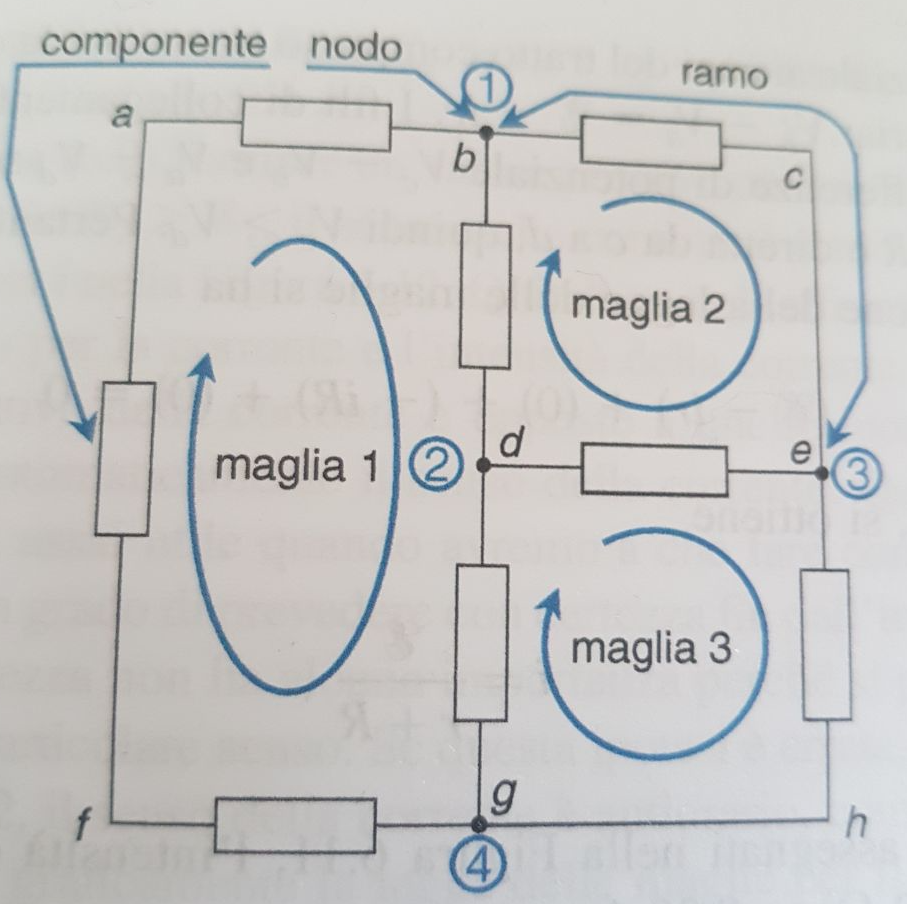
\includegraphics[width=0.5\textwidth]{schema-circuito.png}
  \caption{Schema di un circuito}
  \label{fig:schema_circuito}
\end{figure}

\vspace{1em}
\noindent
È immediato evincere che un \textbf{nodo} è un punto nel quale convergono almeno tre conduttori. La parte di circuito tra due nodi consecutivi è detto \textbf{ramo}. Una \textbf{maglia}, invece, è un percorso chiuso che parte da un nodo e giunge al medesimo nodo dopo aver attraversato vari elementi circuitali senza percorrere due volte lo stesso ramo.\\
In un circuito, in genere, è possibile individuare numerose maglie differenti tra loro, ma è opportuno considerare le maglie (dette \textbf{indipendenti}) scelte in modo da includere in ciascuna almeno un ramo che non sia incluso nelle altre.\\
Il circuito di Figura \ref{fig:schema_circuito} presenta $4$ nodi in totali (anche se i nodi indipendenti sono uno in meno rispetto ai nodi totali e questo vale sempre) e $3$ maglie indipendenti.

\vspace{1em}
\subsubsection{Legge delle maglie}
La legge delle maglie (II legge di Kirchhoff) stabilisce che la somma delle differenze di potenziale  che si incontrano compiendo un giro completo lungo una qualsiasi maglia di un circuito è nulla. Dal momento che il potenziale è connesso in modo diretto con l'energia potenziale dei portatori di carica, la legge delle maglie è una formulazione della conservazione dell'energia. È quindi possibile scrivere la legge delle maglie nella forma
\[\boxed{\sum_{i=1}^n V_i=0}\]
Ovviamente il potenziale aumenta percorrendo alcuni elementi del circuito (come una batteria da $V_-$ a $V_+$) e diminuisce percorrendone altri (come le resistenze nel senso della corrente, o attraversando una batteria da $V_+$ a $V_-$), ma la somma delle differenze di potenziale lungo un giro completo è nulla. Pertanto si ha che
\begin{itemize}
  \item per le batterie
  \begin{itemize}
    \item se vengono attraversate da $V_-$ a $V_+$ si ha un aumento di tensione;
    \item se vengono attraversate da $V_+$ a $V_-$ si ha una caduta di tensione;
  \end{itemize}
  \item per i resistori
  \begin{itemize}
    \item se vengono attraversati nel verso della corrente, si ha una caduta di tensione;
    \item se vengono attraversati nel verso opposto alla corrente, si ha un aumento di tensione;
  \end{itemize}
\end{itemize}
Nell'analizzare il circuito, conviene innanzitutto stabilire arbitrariamente un verso di percorrenza delle maglie e poi assegnare le correnti nei rami con i loro versi, anche in modo arbitrario. Per convenzione, $I$ è positiva quando il senso della corrente corrisponde alla direzione di moto dei portatori di carica positiva. La soluzione numerica del circuito fornirà i segni delle correnti di ramo.

\vspace{2em}
\noindent
\textbf{Esempio}: Si consideri il circuito seguente

\begin{figure}[H]
  \begin{center}
    \begin{circuitikz}
      \draw (0,0)
      to[V,v=$\xi$] (0,2) % Batteria
      to[short] (0,3)
      to[R=$r$] (0,3) % Resistore 1

      to[R=$R_2$] (2,-0.5) % Resistore 2
      to[short] (2,-1)
      to[short] (0,-1)
      to[short] (0,2);
    \end{circuitikz}
    \caption{Resistenze in serie}
  \end{center}
\end{figure}

\vspace{1em}
\noindent
Ovviamente in questo caso si ha una sola maglia che si percorre in senso orario. Per la II legge di Kirchhoff si ha che
\[(V_b-V_a)+(V_c-V_b)+(V_d-V_c)+(V_a-V_d)=0\]
ma naturalmente si ha che
\[\xi - Ir + 0 - I R + 0 = 0\]
per cui si ottengono i due risultati noti $\xi = I \cdot (R+r)$ e quindi $I = \dfrac{\xi}{R+r}$.\\
Se ora si percorre la maglia in senso contrario, si scrive sempre $-Ir$ e $-IR$, ma siccome la batteria si percorre da $V_+$ a $V_-$ si ottiene $-\xi$. Pertanto l'equazione che si ottiene è
\[-\xi - Ir + 0 - I R + 0 = 0\]
per cui si ottengono i due risultati noti $-\xi = I \cdot (R+r)$ e quindi $I = -\dfrac{\xi}{R+r}$, ossia la corrente ottenuta è negativa: ciò significa che la corrente scorre nel verso opposto a quello di percorrenza della maglia.

\vspace{1em}
\subsubsection{Legge dei nodi}
Nell'analisi dei circuiti che contengono due o più maglie, insieme alla legge delle maglie si utilizza la legge dei nodi. La legge dei nodi (I legge di Kirchhoff) afferma che \textbf{la somma delle intensità di correnti entranti in un nodo è uguale alla somma delle intensità delle correnti uscenti dal medesimo nodo}.\\
Se, infatti, si approssima un nodo come una superficie gaussiana cilindrica, è noto che non si ha accumulo di carica in nessun punto dei fili di collegamento, la legge dei nodi è semplicemente un enunciato della conservazione della carica. Si può scrivere la legge dei nodi nella forma
\[\sum \vert i_\text{entranti} \vert = \sum \vert i_\text{uscenti} \vert\]
È importante osservare che date $n$ equazioni riferite a $n$ nodi, solamente $n-1$ sono le equazioni indipendenti che forniscono informazioni significative.

\vspace{1em}
\noindent
\textbf{Esercizio}: Si consideri il circuito a due maglie seguente:

\begin{figure}[H]
  \begin{center}
    \begin{circuitikz}
      \draw (0,0)
      to[V,v=$\xi_1$] (0,2) % Batteria
      to[short] (0,3)
      to[R=$R_1$] (2,3) % Resistore 1
      %to[short] (4,3)
      to[R=$R_3$] (5,3) % Resistore 1
      to[short] (5,2)
      to[V,v=$\xi_3$] (5,0)
      to[short] (5,-2)
      to[short] (2.25,-2); % Batteria
      \draw(2.25,3)
      to[short] (2.25,2.5)
      to[V,v=$\xi_2$] (2.25,1) % Batteria
      %to[short] (2.25,0)
      to[R=$R_2$] (2.25,-1) % Resistore 1
      to[short] (2.25,-2)
      to[short] (0,-2)
      to[short] (0,0);
    \end{circuitikz}
    \caption{Circuito con $2$ maglie}
  \end{center}
\end{figure}

\newpage
\noindent
\begin{center}
  16 Novembre 2022
\end{center}
Com'è noto, la legge di Ohm vale solamente per materiali ohmici; allo steso modo, le leggi di Kirchhoff non sono universali. Per comodità si ripropongono nel seguito:
\begin{itemize}
  \item la legge delle maglie afferma che
  \[\sum V = 0\]
  ossia la somma delle differenze di potenziali in una maglia è sempre nulla;

  \item la legge dei nodi afferma che
  \[\sum i_\text{entranti} = \sum i_\text{uscenti}\]
  ossia la somma algebrica delle correnti entranti in un nodo è uguale a quella delle corrente uscenti.
\end{itemize}
Nel caso di corrente alternata, le leggi di Kirchhoff continueranno a valere, ma con delle variazioni: la tensione e la corrente, per esempio, non saranno costanti. È noto che una corrente costante produce un campo magnetico ma non produce effetti magnetici, ossia non si accoppia con il campo elettrico producendo effetti per il circuito.

\vspace{1em}
\noindent
\subsection{Circuiti RC}

\vspace{1em}
\noindent
\subsubsection{Carica di un condensatore}
Si consideri il circuito seguente

\begin{figure}[H]
  \begin{center}
    \begin{circuitikz}
      \draw (0,0)
      to[V,v=$\xi$] (0,2) % Batteria
      to[short] (0,3)
      to[R=$R$] (2,3) % Resistore 
      to[C=$C$] (2,-0.5) % Condensatore
      to[short] (2,-1)
      to[short] (0,-1)
      to[short] (0,0);
    \end{circuitikz}
    \caption{Circuito RC}
  \end{center}
\end{figure}

\vspace{1em}
\noindent
In tale circuito è presente un condensatore con capacità $C$ collegato ins serie ad una resistenza di valore $R$ e una batteria di f.e.m. $\xi$. È nota la relazione seguente
\[i=\dfrac{\dif q}{\dif t}\]
Studiando l'evoluzione temporale di tale circuito si osserva che a $t=0$ si ha $q(t=0) = 0$, così come per $t \to +\infty$ si ottiene $q(t \to +\infty) = \xi \cdot C$.\\
Applicando la legge delle maglie di Kirchhoff e considerando l'unica maglia dello stesso con senso di percorrenza orario, si ha che
\[\sum V = 0 \hspace{1em} \text{ovvero} \hspace{1em} (V_b-V_a)+(V_c-V_d)+(V_d-V_c)+(V_a-V_d) = \xi - i \cdot R - \dfrac{q}{C} + 0=0\]
in cui è presente il segno meno in $- \dfrac{q}{C}$ dal momento che l'armatura positiva incontra prima la corrente rispetto all'armatura negativa secondo il verso di percorrenza scelto, per vui $V_c > V_d$. Ovviamente, poi, al variare di $t$ varia anche la carica $q(t)$: per quanto osservato a $t=0$ si ha $q(t=0) = 0$, così come per $t \to +\infty$ si ottiene $q(t \to +\infty) = \xi \cdot C$.

\vspace{1em}
\noindent
\textbf{Osservazione}: Per studiare l'accumulazione di carica su ciascuna piastra del condensatore si consideri una superficie gaussiana che contiene solamente la piastra positiva. Per la legge di conservazione della carica si ha che
\[\boxed{i=\dfrac{\dif q}{\dif t}}\]
che non risulta essere la definizione dell'intensità di corrente: infatti, tale equazione esprime il fatto che l'intensità di corrente che circola nel circuito è pari alla rapidità con cui la carica viene trasferita da un'armatura all'altra, ovvero alla rapidità con cui il condensatore viene caricato.

\vspace{1em}
\noindent
Pertanto si ottiene il sistema seguente

\[\left\{
  \rowcolors{1}{white}{white}
  \begin{array}{l}
    \xi - i \cdot R - \dfrac{q}{C}=0\\
    i=\dfrac{\dif q}{\dif t}\\
\end{array}\right.\]
Si ottiene, quindi, l'equazione differenziale seguente
\[\xi - \dfrac{\dif q}{\dif t} R - \dfrac{q}{C} = 0 \hspace{1em} \rightarrow \hspace{1em} \dfrac{\dif q}{\xi C - q} = \dfrac{1}{RC} \dif t\]
in cui $\xi$, $C$ e $R$ sono costanti, mentre $q$ dipende da $t$. Per risolvere tale equazione differenziale è conveniente porre $u=\xi C - q$, il che comporta $\dif u = - \dif q$. L'equazione diviene allora
\[\dfrac{\dif u}{u} = - \dfrac{1}{RC} \dif t \hspace{1em} \rightarrow \hspace{1em} \log(u) = - \dfrac{t}{RC} + \text{costante}\]
ovviamente è possibile anche scrivere
\[u = \text{costante} \cdot e^{-\frac{t}{RC}}\]
e ricordando la definizione di $u$ come $u=\xi C - q$, è facile ottenere
\[\xi C - q = \text{costante} \cdot e^{-\frac{t}{RC}}\]
per determinare il valore della costante, sarà sufficiente porre $t=0$, per cui $q(t=0)=0$, ottenendo che costante$=\xi C$; ecco che quindi si è ottenuta la relazione seguente
\[\xi C - q = \xi C \cdot e^{-\frac{t}{RC}} \hspace{1em} \text{ovvero} \hspace{1em} \boxed{q(t) = \xi C \cdot \left(1-e^{-\frac{t}{RC}}\right)}\]
in cui $\xi C = Q$, ossia la carica finale a $t\to+\infty$. Si ottiene, quindi
\begin{itemize}
  \item quando $t=0$, si ha che $q(t=0)=0$;
  \item quando $t=RC$, si ha che $q(t=RC)=\xi C \cdot \left(1-\dfrac{1}{e}\right)$;
  \item quando $t\to+\infty$, si ha che $q(t\to+\infty)=\xi C$, ossia la carica finale.
\end{itemize}
Ma ovviamente non è possibile attendere un tempo infinito prima di vedere il condensatore carico; questo perché non si ha la necessità di caricare totalmente il condensatore, ma ad una percentuale di $C$ pari, per esempio, al $98\%$. Il tempo di attesa si misura con unità di misura $RC=\tau$, chiamato \textbf{tempo scala}: se $\tau$ è grande, il condensatore si carica lentamente, mentre se $\tau$ è piccolo, il condensatore si carica rapidamente; ovviamente, il tempo necessario perché il condensatore raggiunga una data frazione della sua carica finale è determinato esclusivamente da $\tau$.\\
L'intensità di corrente $i$ si trova derivando rispetto al tempo l'equazione precedentemente ottenuta
\[i=\dfrac{\dif q}{\dif t} = \dfrac{\dif }{\dif t} \left[\xi C (1-e^{-\frac{t}{RC}})\right] = \xi C \cdot \left(-\dfrac{1}{RC}\right) \cdot (-e^{-\frac{t}{RC}})\]
ossia
\[\boxed{i=i(t) = \frac{\xi}{R} e^{-\frac{t}{\tau}} = i_0 \cdot e^{-\frac{t}{\tau}}}\]
dove $i_0=\dfrac{\xi}{R}$ è l'intensità di corrente iniziale.

\vspace{1em}
\noindent
\textbf{Osservazione}: Si consideri, ora, il bilancio energetico del circuito, ossia gli scambi di energia che hanno luogo durante la carica del condensatore.\\
\begin{itemize}
  \item Per quanto riguarda la batteria, è nota la relazione $P=Vi$, per cui
  \[U = \int_0^\infty \xi i \dif t = \int_0^\infty \xi \cdot \left(\dfrac{\xi}{r} \cdot e^{-\frac{t}{\tau}} \right) \dif t = \dfrac{\xi^2}{R} \int_0^\infty e^{-\frac{t}{\tau}} \dif t\]
  è facile caire che
  \[\int_0^\infty e^{-\frac{t}{\tau}} \dif t = \left[- \tau \cdot e^{-\frac{t}{\tau}}\right]_0^{\infty} = \tau\]
  pertanto si ha che
  \[U=\frac{\xi^2}{R} \cdot \tau = \frac{\xi^2}{R} \cdot RC = \xi^2 C\]

  \item Per quanto riguarda il condensatore, si ottiene
  \[U = \int_0^\infty i^2 R \dif t = \int_0^\infty \frac{\xi^2}{R^2} \cdot R \cdot e^{-\frac{2t}{\tau}} \dif t = \frac{1}{2} \frac{\xi^2}{R^2} R \cdot RC \cdot \int_0^\infty e^{-x} \dif x = \frac{1}{2} \xi^2 C\]
\end{itemize}

\vspace{1em}
\noindent
\subsubsection{Scarica di un condensatore}
Si consideri il circuito seguente

Si ottiene il sistema seguente
\[\left\{
  \rowcolors{1}{white}{white}
  \begin{array}{l}
    i \cdot R = - \dfrac{q}{C}\\
    i=\dfrac{\dif q}{\dif t}\\
\end{array}\right.\]
pertanto si ottiene
\[i R = - \frac{q}{C} \hspace{1em} \text{ovvero} \hspace{1em} \frac{\dif q}{\dif t} R = - \frac{q}{C} \hspace{1em} \text{ovvero} \hspace{1em} \dfrac{\dif q}{\dif t} = - \frac{q}{RC}\]
riscrivendo la stessa ordinando i termini si ottiene
\[\frac{\dif q}{q} = - \frac{t}{\tau}\]
per cui
\[q(t) = \text{costante} \cdot e^{-\frac{t}{\tau}}\]
in cui, ovviamente per $t=0$ si ottiene che costante$=q(t=0)=Q$, per cui si ottiene
\[q(t) = Q e^{-\frac{t}{\tau}} \hspace{1em} \text{e} \hspace{1em} i(t) = \frac{Q}{\tau} e^{-\frac{t}{\tau}}\]

\vspace{1em}
\noindent
Per quanto riguarda l'energia assorbita dalla resistenza si ottiene
\[U = \int_0^\infty i^2 R \dif t = \frac{Q^2}{R^2C^2} R \frac{\tau}{2} \int_0^\infty \frac{2}{\tau} e^{-\frac{2t}{\tau}} \dif t = \frac{1}{2} \frac{Q^2}{R^2 C^2} R R C = \frac{1}{2} \frac{Q^2}{C}\]

\newpage
\noindent
\begin{center}
  21 Novembre 2022
\end{center}
\section{Campo magnetico}
L'elettricità è stata introdotta parlando del fenomeno della carica elettrostatica, manifestabile strofinando delle bacchette di materiale conduttore e vedendo che esse attiravano dei pezzetti di carta.\\
Similmente per il magnetismo si potrebbe considerare in modo molto classico la calamita naturale, la quale, tuttavia, è difficile da studiare e descrivere rispetto al campo magnetico generato da una corrente che passa attraverso un filo. Oersted si accorse verso la fine dell'$800$ che una corrente passante attraverso un filo fa muovere l'ago della bussola; cioè, in altre parole, un campo magnetico esercita una forza sulle cariche in movimento.

\vspace{1em}
\noindent
\textbf{Esempio}: Preso un tubo catodico su cui si hanno degli elettroni in movimento da sinistra verso destra, la cui traiettoria viene messa in evidenza da uno schermo fluorescente, allora il campo magnetico di una calamita fa deflettere fli elettroni in moto nel tubo.

\vspace{1em}
\noindent
\textbf{Osservazione}: La forza $\vec F$ che il campo magnetico esercita su una carica è sempre perpendicolare alla velocità $\vec v$ e dipende dal vettore campo magnetico $\vec B$; si ottiene, quindi, la \textbf{forza di Lorentz}
\[\boxed{\va{F} = q \va{v} \times \va{B}}\]
ciò significa che $\vec F$ è sempre ortogonale tanto alla velocità quanto al campo magnetico. Non solo, ma la direzione di tale forza dipende dalla carica: se $q$ è positiva, la forza è nella direzione $\va{v} \times \va{B}$, se $q$ è negativa viceversa. In ogni caso l'intensità della forza è data da
\[F = \vert q v B \sin(\theta)\vert\]
dove $\theta$ è l'angolo compreso tra $\vec{v}$ e $\vec{B}$.\\
Mentre per il campo elettrico è stata impiegata la forza di Coulomb per la sua definizione, per il campo magnetico $\vec B$ ciò non è più possibile, in quanto una stessa forza e velocità possono produrre il medesimo campo magnetico.\\
In generale, il campo magnetico è un campo vettoriale che esercita sulla carica in movimento una forza che è pari alla forza di Lorentz.\\
Per misurare, quindi, il campo magnetico, si procede tramite tubo catodico facendo deflettere gli elettroni con una calamita orientata differentemente. L'unità di misura del sistema internazionale SI dell'induzione magnetica è
\[\dfrac{[\text{N}] \cdot [\text{s}]}{[\text{C}] \cdot [\text{m}]} = \dfrac{[\text{N}]}{[\text{A}] \cdot [\text{m}]} = [\text{T}]\]
dove [T] sta per \textbf{tesla}. Un'altra unità di misura di uso comune è il \textbf{gauss} [G], in cui
\[1 \text{ G} = 10^{-4} \text{ T}\] 

\vspace{1em}
\noindent
\textbf{Osservazione 1}: Si noti che il campo magnetico terrestre, in punti prossimi alla sua superficie, pur variando da punto a punto, ha valori di circa $3 \times 10^{-5}$ T, ossia di $0.3$ G.

\vspace{1em}
\noindent
\textbf{Osservazione 2}: Si osservi, inoltre, che la forza di Lorentz non compie mai lavoro sulle cariche in movimento, in quanto sempre ortogonale alla velocità e quindi allo spostamento. Da notare, però, che la forza esercitata sulle cariche all'interno di un conduttore permette di estrarre energia dalle cariche stesse.\\
Ovviamente, quindi, la forza di Lorentz non è conservativa, ma non è una forza dissipativa come la forza di attrito, in quanto non compie mai lavoro sulle cariche.\\
Si osservi che la velocità e il campo magnetico presenti nella formula della forza di Lorentz sono definiti rispetto ad uno specifico sistema di riferimento e variano al variare del sistema di riferimento considerato. Nell'espressione di una forza fondamentale, infatti, non dovrebbe figurare la velocità, o meglio, potrebbe essere presente se essa fosse costante indipendentemente dal sistema di riferimento considerato, ossia la velocità della luce.

\vspace{1em}
\subsection{Forza agente su un conduttore percorso da corrente}
È noto che la densità di corrente era definita come
\[\vec j = q n \vec{v}_d\]
dove $n$ è il numero di portatori di carica per unità di volume. L'intensità di corrente, inoltre, era definita a partire da $\vec j$ come
\[I = j S = nSq v_d\]
Dato, quindi, un conduttore di forma cilindrica, è noto che il suo volume si calcola come
\[V = S \cdot l\]
in cui $S$ è la sezione, mentre $l$ è la lunghezza del filo conduttore considerato. Il numero di portatori di carica, allora, è pari a
\[N=n l S\]
dove $n$ è il numero di portatori di carica per unità di volume. Allora per calcolare al risultante della forza agente su un conduttore percorso da corrente si ha
\[\vec F = \sum_i \vec{F}_i = N \vec{F}_q = N q \vec{v}_d \times \vec B = nl S q \vec{v}_d \times \vec B\]
in cui si può osservare come
\[nl Sq \vec{v}_d = \vec l \cdot I\]
per come è stata espressa la corrente $I$ all'inizio. Il vettore $\vec l$ sarà tangente al filo e con medesima direzione del vettore velocità di deriva $\vec{v}_d$.\\
In questo modo si ottiene che la forza risultante è data da
\[\boxed{\vec F = I \vec l \times \vec B}\]

\vspace{1em}
\noindent
\textbf{Osservazione}: Ovviamente, tale descrizione funziona solamente se il filo è dritto e rettilineo. Se esso curva non è più possibile associarvi una direzione tramite un solo vettore $\vec l$. La soluzione è quella di scomporre il filo curvilineo in piccole sezioni a cui associare un vettore direzione infinitesimo $\dif \vec l$, per cui si ottiene la \textbf{II legge elementare di Laplace}:
\[\boxed{\dif \vec F = I \dif \vec l \times \vec B}\]
La forza magnetica agente su un segmento di lunghezza finita di un conduttore percorso da corrente si ottiene sommando le fore agenti su ciascun elemento del conduttore, cioè integrando sulla lunghezza della conduttore
\[\vec F = \int_0^L I \dif \vec l \times \vec B\]
in cui $\vec B$ è approssimabile ad una costante nel tratto di conduttore infinitesimo preso in considerazione.

\vspace{2em}
\noindent
\textbf{Esercizio}: Una sfera metallica di raggio $R_1=9.7$ cm è circondata da uno strato metallico sferico e concentrico, di raggio interno $R_2=22.1$ cm.\\
Entrambi i conduttori sono caricati rispettivamente a $+Q$ e $-Q$, con $Q=1.24 \hspace{1em} \mu$C. Su di esse poggiano (allineate lungo una retta radiale) due sferette isolanti, di massa $m=1$ g e raggio trascurabile, caricate rispettivamente a $-q$ e $+q$, con $q=7.42$ nC.

\begin{itemize}
  \item Trascurando le sferette, calcolare il campo elettrico in ogni punto tra le due armature, specificando il suo valore numerico a $R_1$.
  
  \vspace{2em}
  \noindent
  Per la legge di Gauss si ha che
  \[E(r) \cdot 4 \pi r^2 = \dfrac{Q}{\epsilon_0} \hspace{1em} \rightarrow \hspace{1em} \vec{E}(r) = \dfrac{Q}{4 \pi \epsilon_0} \hat r \hspace{1em} R_1<r<R_2\]

  \item Le sferette vengono avvicinate fino a distanza $d=4$ mm seguendo un cammino radiale di uguale lunghezza per entrambe, quindi collegate tra loro con un bastoncino rigido e isolante fino a formare un dipolo, e ruotate in modo che il bastoncino stia sulla superficie equipotenziale. Quanta energia serve per raggiungere questa configurazione? (Si chiama $r_+$ ed $r_-$ le posizioni delle due cariche come in figura, $r_m$ la posizione del centro di massa.)

  \vspace{2em}
  \noindent
  Calcolando la differenza di potenziale della carica $+q$ tra $R_1$ e $r_-$ si ha
  \[\Delta V = V_- - V_1 = -\int_{R_1}^{r_-} \vec E \cdot \dif \vec l\]
  Dopodiché se ne calcola l'energia associata, da qui
  \[\Delta U = \dfrac{\Delta V}{q}\]
\end{itemize}

\newpage
\noindent
\begin{center}
  22 Novembre 2022
\end{center}
In precedenza è stato introdotta la forza di Lorentz, calcolata come segue
\[\vec F = q \vec v \times \vec B\]
che può essere impiegata anche come definizione di campo magnetico. Per la II legge elementare di Laplace, si ha che la forza di Lorentz agente su un conduttore percorso da corrente è
\[\dif \vec F = I \dif \vec l \times \vec B\]
in cui si considera $\vec l$ come un vettore che descrive la direzione di un conduttore. 

\vspace{1em}
\subsection{Momento agente su una spira percorsa da corrente}
Dato che un campo di induzione magnetica esercita una forza su un filo percorso da corrente, esso può produrre anche un momento. Di particolare interesse è il momento esercitato su una spira di filo metallico imperniata su un asse e percorsa da una corrente. Il moto rotatorio prodotto da tale momento è alla base del motore elettrico.\\
Per rappresentare i vettori entranti e uscenti dal foglio, si usa la convenzione seguente
\begin{itemize}
  \item $\odot   \text{ vettore uscente}$
  \item $\otimes \text{ vettore entrante}$
\end{itemize}
Si consideri, allora, una spira rettangolare percorsa da corrente, immersa in un campo magnetico uniforme entrante nel foglio. Il vettore superficie $\vec S$ è perpendicolare al piano della spira e ha verso definito dalla regola della mano destra rispetto al senso di circolazione della corrente nella spira, che è orario per ipotesi.\\
Si sceglie un asse nel piano della spira e perpendicolare al campo elettrico $\vec B$, indicato con $OO'$. È chiaro che, se la spira è imperniata su tale asse, il momento tende a far sì che la spira ruoti intorno all'asse.\\
Per determinare l'entità delle forze agenti sulla spira di forma rettangolare dovute al passaggio della corrente $I$ e al campo elettrico $\vec B$ si impiega la II legge elementare di Laplace
\[\dif \vec F = I \dif \vec L \times \vec B\]
Si vede facilmente che le forze saranno dirette tutte ortogonalmente alla spira con verso uscente dalla stessa; ovviamente, le forze dirette parallelamente all'asse di rotazione non producono alcun momento rispetto a tale asse, mentre quelle dirette ortogonalmente alla stessa produrranno un momento di forza 
\[\vec \tau = \vec r \times \vec F\]
ma siccome il braccio $r$ è pari alla metà della larghezza $w$ della spira, si ha che
\[\tau = \dfrac{w}{2} I l B \sin(\theta)\]
in cui $\theta$, in generale, è l'angolo compreso tra il braccio e la forza stessa. Ovviamente, il momento di forza prodotto dalla seconda forza non parallela all'asse di rotazione è uguale al primo, per cui il momento totale è
\[\tau = \tau_1+\tau_2= w \cdot I l B \sin(\theta) = I S B \sin(\theta)\]
dove si è tenuto conto, ovviamente, che l'area della spira rettangolare è $S=wl$. Quindi il vettore momento agente sulla spira per effetto di un campo magnetico uniforme è
\[\boxed{\vec \tau = I \vec S \times \vec B}\]

\vspace{1em}
\noindent
\textbf{Osservazione}: Si osservi che nella configurazione precedentemente considerata, la risultante delle forze agenti è nulla, per cui non si hanno deformazioni della spira di nessuna sorta.

\vspace{1em}
\noindent
L'effetto del momento meccanico è quello di allineare $\vec S$ con il campo magnetico $\vec B$. Ovviamente, la direzione di $\vec \tau$ dipende dal senso di percorrenza della corrente, per cui bisogna usare la regola della mano destra: se la corrente scorre in senso orario, il verso del vettore superficie $\vec S$ è entrante; se la corrente scorre in senso antiorario, il verso del vettore superficie $\vec S$ è uscente.

\vspace{1em}
\noindent
\textbf{Osservazione}: Se al posto di considerare una sola spira, si può prendere in considerazione una bobina con $N$ spire. Se la bobina è avvolta in modo che le spire siano ditta, ciascuna di esse giace sostanzialmente in un piano e tali piani sono paralleli, di modo che i vettori superficie per le varie spire siano tutti uguali a $\vec S$. Se il momento agente su ciascuna spira è $\vec \tau = I \vec S \times \vec V$, allora il momento della forza magentica agente sulla bobina in un campo magnetico uniforme è
\[\vec \tau = N I \vec S \times \vec B\]
per la similitudine di tale fenomeno con il dipolo elettrico, si definisce il \textbf{momento di dipolo magnetico di una bobina percorsa da corrente} è
\[\vec m = NI \vec S\]
Generalizzando l'equazione del momento della forza magnetica agente su una bobina si ottiene che 
\[\vec \tau = \vec m \times \vec B\]
Come nel caso del dipolo elettrico, c'è una energia potenziale associata a un dipolo magnetico immerso in un campo magnetico. Tale energia potenziale è
\[U = - \vec m \cdot \vec B\]
che è, esattamente come per il dipolo, una energia potenziale associata alla rotazione dello stesso dipolo rispetto al campo considerato (elettrico nel primo, magnetico nel secondo).

\vspace{1em}
\noindent
\textbf{Esercizio}: In un condensatore piano, carico con $\Delta V=400$ V e isolato, con armature di area $A=200$ cm$^2$ e distanti $d=0.80$ cm, viene inserita una lastra di rame di spessore $b=0.20$ cm e di area identica a quella delle armature, in modo da stare a metà tra le stesse.

\begin{itemize}
  \item Calcolare la capacità del condensatore dopo aver introdotto la lastra.

  \vspace{1em}
  \noindent
  Tale configurazione è approssimabile ad avere due condensatori in serie, ciascuna con capacità
  \[C_{1,2} = \epsilon_0 \cdot \dfrac{A}{\dfrac{d-b}{2}}\]
  la capacità equivalente sarà
  \[C_\text{eq} = \epsilon_0 \cdot \dfrac{A}{d-b}\]

  \item Calcolare il lavoro necessario per introdurre la lastra, con il suo segno.
  
  \vspace{1em}
  \noindent
  Il lavoro necessario è dato da
  \[\Delta W = - \Delta U = -\dfrac{1}{2} \dfrac{\Delta Q^2}{C}\]
  Supponendo che il condensatore sia staccato, allora $\Delta Q$ sarà costante, per cui
  \[\Delta U = \dfrac{1}{2} Q^2 (C_\text{eq} - C_\text{ini})^{-1}\]

  \item Si dica come cambia la capacità se la lastra non è esattamente al centro delle due armature. Nella risposta, tenete conto del rischio di rottura del dielettrico.

  \vspace{1em}
  \noindent
  La capacità equivalente non varierà se la lastra non è esattamente a metà tra le due armature.\\
  Il campo elettrico è tanto più grande quanto più si avvicinano le lastre e se esso diviene maggiore del campo elettrico limite
  \[E_{\max} \cong 3 \times 10^6 \dfrac{\text{V}}{\text{m}}\]
  il dielettrico si rompe.
\end{itemize}

\newpage
\noindent
\begin{center}
  23 Novembre 2022
\end{center}
È stata introdotta, in precedenza, la forza di Lorentz come
\[\vec F = q \vec v \times \vec B\]
che è stata assunta come definizione di campo magnetico. Applicando tale legge alla forza agente su un conduttore attraversato da corrente si ottiene la II legge elementare di Laplace
\[\dif \vec F = I \dif \vec l \times \vec B\]
Tale formula, applicata ad una bobina attraversata da corrente, produce un momento torcente
\[\vec \tau = NI \vec S \times \vec B\]
Non solo, ma è possibile associare a tale spira anche un momento di di dipolo magnetico
\[\vec m = N I \vec S\]
per cui è possibile determinare la torsione come
\[\vec \tau = \vec m \times \vec B\]

\vspace{1em}
\noindent
\subsubsection{Momento magnetico e meccanico di una spira di forma arbitraria}
Si supponga, ora, di considerare una spira non più rettangolare, ma di una forma generica. Ci si chiede, ora, se la legge per il momento di forza $\tau$ continui a valere anche per una spira generica. Si procede, allora, a racchiudere la superficie data in un plurirettangolo, ossia in un insieme di rettangoli di piccole dimensioni ciascuna contenente una sezione della spira. Si sono ottenute, così facendo, tante piccole spire rettangolari in cui la corrente scorre nello stesso verso imposto dalla superficie irregolare: ovviamente, lungo i lati comuni a due spire (ossia i lati \quotes{interni}) si sovrappongono correnti di verso opposto, cosicché l'intensità di corrente in essi è nulla; per la II legge elementare di Laplace, quindi, le forze che agiscono sui lati interni compaiono in due spire e sempre con verso opposto: anche il momento meccanico totale che agisce sulla spira può essere calcolato come somma (vettoriale) dei momenti meccanici che agiscono su ciascuna spira rettangolare:
\[\vec \tau = \sum \vec{\tau}_i = \sum \left(\vec{m}_i \times \vec B\right) = \left(\sum \vec{m}_i\right) \times \vec B\]
Il momento di dipolo magnetico della spira, quindi, è uguale alla somma (vettoriale) dei momenti di dipolo magnetico delle spire rettangolari:
\[\vec m = \sum \vec{m}_i = \left(\sum I \vec{S}_i\right) = I\left(\sum \vec{S}_i\right)\]
Facendo, quindi, tendere a $0$ le dimensioni delle spire si ottiene che
\[\vec \tau = I \cdot \left(\iint_\mathcal{S} \dif \vec S \right) \times \vec B\]

\vspace{2em}
\noindent
\textbf{Osservazione 1}: Si supponga che il campo magnetico $\vec B$ non sia costante, ma sia variabile; ovviamente tale condizione implica che non si possa portare fuori $\vec B$ dall'integrale, calcolando
\[\vec \tau = I \cdot \left(\iint_{\mathcal{S}_\gamma} \dif \vec S \times \vec B(\vec r)\right)\]

\vspace{2em}
\noindent
\textbf{Osservazione 2}: Si consideri, ora, una spira non più piana, ma che si sviluppa nello spazio; allora la modalità di definire la superficie che presenta come frontiera la spira non è univoca: in altre parole, ci sono infinite superfici che presentano una medesima frontiera. Non esiste, in realtà, un criterio per scegliere una superficie piuttosto che un'altra, ma molto spesso, nei casi che si analizzeranno, la soluzione non cambia.

\vspace{1em}
\noindent
\textbf{Esempio}: Si consideri una spira tridimensionale a forma di sedia. Allora è possibile scomporre tale spira in due rettangoli (cosicché le forze agenti sul lato interno si annulleranno); allora, in questo modo, sarà possibile calcolare i momenti di dipolo magnetico per ciascuna sotto-spira
\begin{align*}
  &\vec{m}_1=I \cdot \vec{S}_1\\
  &\vec{m}_2=I \cdot \vec{S}_2\\
\end{align*}
per cui il momento di dipolo magnetico totale è
\[\vec m = \vec{m}_1 + \vec{m}_2 = I \cdot (\vec{S}_1 + \vec{S}_2)\]
e quindi il momento meccanico totale sarà
\[\vec \tau = I \cdot (\vec{S}_1 + \vec{S}_2) \times \vec B\]

\vspace{1em}
\subsection{Galvanometro}
È noto che il momento meccanico associato ad una bobina è
\[\vec \tau = N I \vec S \times \vec B = \vec m \times \vec B\]
allora, se si considera una molla a forma di spirale che reagisce ad una sollecitazione di momento meccanico in modo lineare, secondo la legge
\[\tau = - k \theta\]
Nella geometria del campo magnetico costruito, si ha che l'angolo tra il campo magnetico e il momento di dipolo magnetico è pari a $90^\circ$, sempre. Pertanto, il valore del momento di forza $\tau$ si calcola come segue
\[\tau = m B \sin(\theta) = m B =  NIS B\]
Si ottiene quindi
\[k \theta = NIS B \hspace{1em} \rightarrow \hspace{1em} \theta = I \cdot \dfrac{NSB}{k}\]

\vspace{1em}
\subsection{Moto di cariche libere in presenza di $\vec E$ e di $\vec B$}
Una particella carica immersa in un campo elettrico $\vec E$ e in un campo magnetico $\vec B$ è sottoposta a due forze, quella di Coulomb e quella di Lorentz, per cui
\[\vec F = q \vec E + q \vec v \times \vec B\]
in cui il primo è un prodotto scalare, mentre il secondo è un prodotto vettoriale; le due forze addendi, inoltre, sono diversi come natura, in quanto la forza di Coulomb compie lavoro, la seconda, quella di Lorentz, non compie mai lavoro.\\
Analizzando dapprincipio il caso in vi sia una particella carica in moto all'interno di un campo magnetico uniforme e in assenza di campo elettrico. Nell'ipotesi in cui il campo magnetico $\vec B$ sia uscente dalla pagina e che la velocità $\vec v$ sia, inizialmente, perpendicolare al campo magnetico. Ciò significa che la forza di Lorentz $\vec F$ risultante è ortogonale al vettore velocità $\vec v$ (ma i due vettori giacciono sul medesimo piano) e al vettore campo magnetico $\vec B$. Se la forza magnetica è l'unica forza che agisce sulla particella carica, per la seconda legge di Newton l'accelerazione della particella è perpendicolare alla velocità e giace anch'essa nel piano perpendicolare a $\vec B$. La formula della forza centripeta permette di ottenere
\[F = \dfrac{mv^2}{r} = qvB\]
in cui l'orbita del ciclotrone è proprio
\[R = \dfrac{mv}{qB}\]

\vspace{1em}
\noindent
\textbf{Osservazione}: Se la velocità iniziale non fosse stata ortogonale al campo magnetico, essa si sarebbe potuta scomporre in due direzioni: parallela al campo magnetico e ortogonale ad esso. Ovviamente la componente parallela della velocità non sarebbe stata soggetta alla forza di Lorentz e quindi non avrebbe subito accelerazione; pertanto
\begin{itemize}
  \item particelle che si muovono parallelamente al campo magnetico si muovono di moto rettilineo uniforme;
  \item particelle che si muovono ortogonalmente al campo magnetico si muovono di moto circolare uniforme.
\end{itemize}

\vspace{1em}
\noindent
\subsubsection{Selettore di velocità}
Si immerga una carica positiva all'interno di un condensatore piano (con armatura caricata negativamente verso l'alto) e con un campo magnetico uniforme uscente dal foglio.\\
Allora si ha che la forza di Coulomb è diretta verso l'alto, mentre la forza magnetica è diretta verso il basso, per cui si ottiene
\[F_\text{tot} = qE - qvB\]
Nell'ipotesi in cui $v$ sia tale che $F_\text{tot}=0$ si ottiene
\[F_\text{tot} = q \cdot (E - vB) = 0\]
Dovendo essere $q \neq 0$, deve essere necessariamente
\[E = vB \hspace{1em} \rightarrow \hspace{1em} v = \dfrac{E}{B}\]
per cui variando opportunamente $\vec E$ e $\vec B$ si può ottenere la velocità che si desidera.

\vspace{1em}
\noindent
\subsubsection{Spettrografo di massa}
Si consideri un campo magnetico uniforme entrante nel foglio e un selettore di velocità che spara elettroni ortogonalmente al campo magnetico e sul piano del foglio; in questo modo la particella segue una traiettoria circolare di raggio $r$, con un accelerazione centripeta
\[a=\dfrac{v^2}{r}\]
mentre la forza che agisce sulla carica è, in modulo,
\[F=qvB\]
per la seconda legge di Newton si ha che $\vec F = m \vec a$, per cui è possibile scrivere
\[qvb = m \cdot \dfrac{v^2}{r} \hspace{1em} \rightarrow \hspace{1em} m=\dfrac{q B r}{v}\]
ma il modulo di velocità della particella è determinato dal selettore di velocità, con formula $v=\dfrac{E_0}{B_0}$, per cui
\[m = \dfrac{q B B_0 r}{E_0}\]
Se ora si considerano due particelle, a parità di valori di $q$, $E_0$, $B_0$ e $B$ si ottiene
\[\dfrac{m}{m_0} = \dfrac{r}{r_0}\]

\newpage
\noindent
\begin{center}
  28 Novembre 2022
\end{center}
\section{Campo magnetico e correnti}
Il campo magnetico esercita sulle cariche in movimento una forza che dipende dalla velocità delle cariche, secondo la Legge di Lorentz seguente
\[\vec F = q \vec v \times \vec B\]

\vspace{1em}
\subsection{Legge di Biot e Savart}
Immediatamente dopo la scoperta di Oersted che una corrente elettrica è sorgente di un campo magnetico, esperimenti condotti da André-Marie Ampere, da Jean-Baptise Biot e Félix Savart portarono a quella che oggi è nota come \textbf{legge di Biot e Savart} o anche come \textbf{I Legge elementare di Laplace}. Tale legge determina, in un punto dello spazio, il campo di induzione magnetica generato da una distribuzione di correnti elettriche.\\
La legge di Coulomb, unita alla definizione di campo elettrico, fornisce il campo elettrico prodotto da una distribuzione di carica, secondo la formula
\[\dif \vec E = \dfrac{1}{4 \pi \epsilon_0} \dfrac{\dif q}{r^2} \hat r\]
dove $r$ è la distanza dell'elemento di carica dal punto $P$ e $\hat r$ è il versore diretto dalla carica al punto $P$.\\
Considerando, ora, una distribuzione di corrente, un elemento di corrente $I \dif \vec l$ produce un contributo $\dif \vec B$ al campo di induzione magnetica in un punto $P$. Se $r$ rappresenta la distanza dell'elemento di corrente dal punto $P$, e il valore $\hat r$ è diretto dall'elemento di corrente al punto $P$, la \textbf{legge di Biot e Savart} per un elemento infinitesimo di corrente è
\[\boxed{\dif \vec B = \dfrac{\mu_0}{4 \pi} \dfrac{I \dif \vec l \times \hat r}{r^2}}\]
La direzione di $\dif \vec B$ è data dalla direzione del prodotto vettoriale $I \dif \vec l \times \hat r$ ed è perpendicolare tanto all'elemento di corrente $I \dif \vec l$ quanto al versore $\hat r$, mentre il verso è dato dalla regola della mano destra.\\
Il modulo di $\dif B$ è
\[\dif B = \dfrac{\mu_0}{4\pi} \dfrac{I \dif l \sin(\theta)}{r^2}\]
dove $\theta$ è l'angolo compreso tra le direzioni di $I \dif \vec l$ e $\hat r$. La costante $\mu_0$ è chiamata \textbf{permeabilità magnetica} del vuoto ed è analoga a $\epsilon_0$, ossia la costante dielettrica del vuoto nell'elettrostatica.\\
A causa delle connessioni che sussistono tra elettricità e magnetismo, i valori di $\epsilon_0$ e $\mu_0$ non sono indipendenti: tali costanti sono legate alla velocità $c$ delle onde elettromagnetiche nel vuoto dalla relazione
\[c=\dfrac{1}{\sqrt{\epsilon_0 \mu_0}}\]
In particolare, il valore di $\mu_0$ è pari a
\[\mu_0 = 4 \pi \times 10^{-7} \text{ T m A}^{-1}\]
che è un valore esatto, in quanto la $17^a$ conferenza generale di Pesi e Misure del $1983$ ha deciso di definire in modo esatto $c=2.99792458 \times 10^8 \dfrac{\text{m}}{\text{s}}$, per cui per la relazione di cui sopra $\mu_0$ si ricava in modo esatto, secondo la definizione esatta di $c$.

\vspace{2em}
\subsubsection{Campo magnetico di un filo rettilineo indefinitamente lungo percorso da corrente}
Si consideri un filo parallelo all'asse $x$ percorso da una corrente di intensità $I$ con verso concorde con l'asse $x$. L'elemento di corrente $I \dif l$ fornisce il contributo $\dif \vec B$ al campo di induzione magnetica nel punto $P$. Ovviamente, per la regola della mano destra si ha che $\dif \vec B$ è uscente dal piano della figura.\\
Il modulo del campo magnetico è
\[\dif B = \dfrac{\mu_0}{4\pi} \dfrac{I l \sin(\theta)}{r^2}\]
dove $r$ è la distanza dell'elemento di corrente $\dif \vec l$ da $P$, ossia l'ipotenusa del triangolo di cateti $R$ e $x$, per cui
\[\dif B = \dfrac{\mu_0}{4\pi} \dfrac{I l \sin(\theta)}{r^2} = \dfrac{\mu_0}{4\pi} \dfrac{I l \sin(\theta)}{R^2+x^2}\]
Naturalmente, poi, è possibile esprimere
\[\sin(\theta)=\sin(\pi-\theta)=\dfrac{R}{\sqrt{R^2+x^2}}\]
per cui si ottiene, in definitiva l'espressione seguente
\[\dif B = \dfrac{\mu_0}{4\pi} \dfrac{I R \dif x}{\left(x^2+R^2\right)^{\frac{3}{2}}}\]
Pertanto si ottiene il campo magnetico è
\[\int_{-\frac{l}{2}}^{\frac{l}{2}} \dfrac{\mu_0}{4\pi} \dfrac{IR \dif x}{(x^2+t^2)^{\frac{3}{2}}} = \frac{\mu_0}{4\pi} IR \cdot \dfrac{L}{R \cdot \sqrt{R^2+\dfrac{L^2}{4}}}\]
pertanto, quando $L \to +\infty$ si ottiene
\[\boxed{B=\dfrac{\mu_0 I}{2 \pi R}}\]

\vspace{2em}
\subsubsection{Campo magnetico sull'asse di una spira percorsa da corrente}
Si consideri un elemento di corrente di una spira circolare, il quale produce un contributo $\dif \vec B$ al campo di induzione magnetica in un punto sull'asse della spira. Ovviamente, i vettori $I \dif \vec l$ e $\hat r$ sono perpendicolari.\\
Il modulo di $\dif \vec B$ è lo stesso per ogni elemento di corrente della spira, ma la direzione dei vari contributi è diversa. Si scompone, quindi, $\dif \vec B$ nelle componenti $\dif \vec B_x = \dif B \cos(\phi)$, l'ungo l'asse della spira e $\dif B_\perp = dB \sin(\phi)$, perpendicolare all'asse. Per ragioni di simmetria, l'integrale esteso alla spira della componente perpendicolare $\dif B_\perp$ è nullo. Si noti, quindi, che l'elemento di corrente $I \dif \vec l$ e il versore $\hat r$ sono perpendicolari, per cui $\sin(\theta)=1$. Pertanto si ha che
\[\dif B_x = \dfrac{\mu_0 I \dif l \cos(\theta)}{4 \pi \cdot \left(x^2+a^2\right)}\]
sfruttando il fatto che $r^2=x^2+a^2$. Nell'effettuare l'integrazione lungo la spira, ciascun fattore dell'integrando è costante e può essere portato fuori dal segno di integrale, cosicché rimane
\[\int \dif l = l = 2 \pi a\]
che è semplicemente la circonferenza della spira. Si ottiene quindi
\[B_x=\dfrac{\mu_0 I 2 \pi a \cos(\phi)}{4 \pi (x^2+a^2)}\]
Osservando che
\[\cos(\phi) = \dfrac{a}{r} = \dfrac{a}{(x^2+a^2)^{\frac{3}{2}}}\]
per cui si ottiene che
\[B_x = \dfrac{\mu_0 I 2 \pi a^2}{4 \pi (x^2+a^2)^{\frac{3}{2}}}\]
Tale risultato può essere espresso in forma più semplice ricorrendo al momento di dipolo magnetico $\vec m = I \vec S$. Si noti, poi, che il fattore $\pi a^2$ che compare nel numeratore è il valore $S$ dell'area della spira e che il prodotto $I\pi a^2$ è il modulo $m=IS$ del momento di dipolo magnetico della spira percorsa da corrente. Si noti, inoltre, che $\vec B$ e $\vec m$ presentano la medesima direzione, quella del semiasse $x$ positivo. Si ha, quindi
\[\vec B = \dfrac{\mu_0}{2\pi} \dfrac{\vec m}{(x^2+a^2)^{\frac{3}{2}}}\]
Nei punti lontani dalla spira, dove $\vert x\vert >> a$, si ottiene che
\[(x^2+a^2)^{\frac{3}{2}} \cong (x^2)^{\frac{3}{2}} = \vert x\vert^3\]
Pertanto, l'intensità del campo è data approssimativamente
\[B \cong \dfrac{\mu_0 m}{2 \pi \vert x \vert^3}\]
La dipendenza di $B$ dall'inverso del cubo della distanza dalla spira (lontano dalla spira) è caratteristica di un campo di dipolo. Infatti, si confronti il risultato ottenuto per $\vec B$ con quello ottenuto per $\vec E$ sull'asse di un dipolo elettrico
\[E \cong \dfrac{p}{2 \pi \epsilon_0 z^3}\]

\vspace{2em}
\noindent
\textbf{Osservazione}: Si può dimostrare formalmente che l'analogia ottenuta vale in generale: il campo magnetico generato da una spira percorsa da corrente percorsa da corrente in punti lontani dalla spira è un campo di dipolo:
\[\boxed{\vec B (\vec r) = \dfrac{\mu_0}{4 \pi} \cdot \dfrac{3 (\vec m \cdot \hat r) \hat r - \vec m}{r^3}}\]
in cui se $\vec m$ e $\hat r$ sono allineati, come nel caso preso in esame, si ottiene
\[\vec B(\vec r) = \dfrac{\mu_0}{4 \pi} \cdot \dfrac{3 \vec m - \vec m}{r^3} = \dfrac{2 \mu_0 \vec m}{4 \pi r^3}\]

\vspace{2em}
\noindent
\textbf{Osservazione}: È noto che un filo infinito crea un campo magnetico che si avvolge attorno al filo. Per conoscere il flusso di tale campo magnetico è possibile calcolarlo come differenza tra le linee entranti e quelle uscenti dalla superficie presa in considerazione. Ma siccome le linee di campo magnetico si avvolgono sempre su se stesse, ovviamente il flusso totale attorno ad una qualsiasi superficie chiusa è sempre nullo.\\
Pertanto, al posto di calcolare il flusso, ha più significato parlare di \textbf{circuitazione}, calcolabile come segue
\[\oint \vec B \cdot \dif \vec r = \mu_0 I\]
che si esprime come \textbf{legge di Ampere}.

\newpage
\noindent
\begin{center}
    29 Novembre 2022
\end{center}
Si consideri una corrente che scorre in un filo conduttore, allora il campo magnetico, espresso secondo la legge di Biot e Savart, è
\[\dif \vec B = \frac{\mu_0}{4 \pi} \cdot \frac{I \dif \vec l \times \hat r}{r^2}\]
anche nota come I legge elementare di Laplace. Vi sono motivazioni intrinseche per andare oltre tale legge, come fatto per la legge di Coulomb, la quale è stata seguita dall'espressione della legge di Gauss.\\
In particolare, è noto che il flusso netto di un campo vettoriale è dato dalla differenza tra le linee entranti e quelle uscente dal campo vettoriale.\\
Per esempio, nel caso del campo magnetico generato da un lungo filo conduttore, si può calcolare il flusso come
\[\oint \vec B \dif \vec r\]
dal momento che il campo magnetico e il vettore $\vec r$ sono sempre paralleli, in quanto le linee del campo magnetico ha una direzione circolare e si chiudono sempre su se stesse; percorrendo tali linee nella direzione del campo magnetico, ovviamente si ottengono sempre vettori tangenti la curva, fra loro paralleli; pertanto il prodotto scalare è massimo, per cui
\[\oint \vec B \dif \vec r = \oint B \cdot \dif r = \oint \dfrac{\mu_0 I}{2 \pi R} \dif r = \dfrac{\mu_0 I}{2 \pi R} \oint \dif r = \dfrac{\mu_0 I}{2 \pi R} \cdot 2\pi R = \mu_0 I\]
in quanto l'integrale chiuso sulla circonferenza di porzioni infinitesimali di lunghezza della stessa è proprio la lunghezza della circonferenza stessa. Si ottiene, quindi, la \textbf{circuitazione del campo magnetico}, che presenta un'espressione molto compatta, ottenuta, però, nel caso non reale di un filo indefinitamente nullo.
Supponendo, ora, di muoversi non più sulle circonferenze concentriche del campo magnetico, ma su un qualsiasi percorso chiuso, si può sempre scomporre il vettore spostamento $\dif \vec r$ nelle sue componenti parallela (ossia tangenziale) al campo magnetico e ortogonale (ossia radiale) al campo magnetico, che non contribuisce al prodotto scalare, ovvero
\[\vec B \cdot \dif \vec r = \vec B \cdot (\dif \vec r_{\parallel} + \dif \vec r_\perp) = \vec B \cdot \dif \vec r_{\parallel}\]
Si osservi, poi, che $\dif \vec r_{\parallel}$ può essere espresso come
\[r_\parallel = R \cdot \sin(\theta)\]
con $R$ la distanza del punto sul cammino rispetto al centro. Per angoli piccoli, quindi, si può scrivere
\[\dif \vec r_\parallel = R \dif \theta\]
per cui, in conclusione, si ottiene che
\[\vec B \cdot \dif \vec r_\parallel = \dfrac{\mu_0 I}{2 \pi R} \cdot R \dif \theta = \dfrac{\mu_0 I}{2\pi} \dif \theta\]
Procedendo, ora, all'integrazione si ottiene
\[\oint \vec B \cdot \dif \vec r = \dfrac{\mu_0 I}{2 \pi} \cdot \int_0^{2\pi} \dif \theta = \frac{\mu_0 I}{2 \pi} \cdot 2\pi = \mu_0 I\]

\vspace{1em}
\noindent
\textbf{Osservazione 1}: Si osservi che cambiando il verso di percorrenza del filo non cambia il risultato, in quanto il coseno dell'angolo tra $\vec B$ e $\vec r_\parallel$ sarà negativo, ma anche la corrente avrà segno $-$, per cui si otterrà il medesimo risultato.\\

\vspace{1em}
\noindent
\textbf{Osservazione 2}: Si potrebbe, però, anche osservare che non è detto che il circuito stia sul piano, ma potrebbe essere sullo spazio: tuttavia, la componente verticale è sempre ortogonale al campo magnetico, per cui il suo contributo al prodotto scalare è sempre nullo, per cui si ottiene ancora il risultato di partenza.

\vspace{1em}
\noindent
\textbf{Osservazione 3}: Nell'ipotesi in cui il circuito non contenga il filo, ossia il filo di forma arbitraria che si va percorrendo non comprenda nella sua superficie interna il filo conduttore che genera il campo magnetico, si dovrà calcolare l'integrale
\[\oint \vec B \dif \vec r = \frac{\mu_0 I}{2 \pi} \left[\int_{\theta_1}^{\theta_2} + \int_{\theta_2}^{\theta_1} \dif \theta\right] = 0\]
in quanto quando si percorre il circuito radiale che non contiene il filo fino ad un cerco angolo si sta andando nello stesso verso della corrente, ma tornando indietro si sta percorrendo la stessa differenza di angoli, ma in verso contrario alla corrente, per cui i due integrali sommano a $0$.

\vspace{1em}
\noindent
\textbf{Osservazione 4}: Pertanto, in conclusione, si ha che 
\[\oint \vec B \cdot \dif \vec r = \dfrac{\mu_0 I}{2 \pi} \cdot \int_0^{2\pi} \dif \theta = \frac{\mu_0 I}{2 \pi} \cdot 2\pi = \mu_0 I\]
è un risultato valido solamente nell'ipotesi in cui la \textbf{corrente è concatenata al circuito}.\\
Altrimenti, se la corrente non è concatenata al circuito si ottiene che
\[\oint \vec B \cdot \dif \vec r = 0\]
Si noti, quindi, la particolare analogia con la legge di Gauss: in questo caso il ruolo della carica viene rivestito dalla corrente, mentre la superficie in questo caso è il circuito.\\
Si osservi che se si considera un circuito che si avvolge più volte attorno al filo, allora il contributo dato al flusso è pari a $\mu_0 I$ moltiplicato tante volte quanti sono gli avvolgimenti attorno al filo.\\
Si ottiene, quindi, la \textbf{legge di Ampere} seguente
\[\boxed{\oint \vec B \cdot \dif \vec r = \mu_0 I_\text{conc}}\]

\vspace{2em}
\noindent
Generalizzando la legge di Ampere al caso in cui vi sono più campi magnetici, si può applicare la legge di sovrapposizione degli effetti
\[\oint (\vec B_1 + \vec B_2) \cdot \dif \vec r = \oint \vec B_1 \cdot \dif \vec r + \oint \vec B_2 \cdot \dif \vec r\]
per cui secondo la legge di Ampere si avrà che
\[\mu_0 \cdot \sum I_\text{conc}\]
in cui si dovrà considerare la somma delle correnti concatenate.\\
In particolare, preso un qualsiasi circuito che presenta come frontiera una curva chiusa $\gamma$, per la legge di Ampere si ha che
\[\oint_\gamma \vec B \cdot \dif \vec r = \mu_0 \cdot I_\text{conc} = \mu_0 \iint_{\mathcal{S}_\gamma} \vec j \cdot \dif \vec S\]

\vspace{2em}
\noindent
\textbf{Osservazione}: Si era osservato che il campo elettrico è conservativo, ossia
\[\oint \vec E \cdot \dif \vec r = 0\]
allora era possibile esprimere tale conservatività con una legge differenziale data
\[\lim_{\Delta \mathcal{S} \to 0} \dfrac{\displaystyle{\int_{xy} \vec E \cdot \dif \vec r}}{\Delta \mathcal{S}} = (\text{rot } \vec E)_z\]
Similmente, nel caso del campo magnetico, avendo a disposizione la legge di Ampere generalizzata
\[\oint_\gamma \vec B \cdot \dif \vec r = \mu_0 \cdot I_\text{conc} = \mu_0 \iint_{\mathcal{S}_\gamma} \vec j \cdot \dif \vec S\]
si può considerare
\[\lim_{\Delta \mathcal{S} \to 0} \dfrac{\displaystyle{\int_{xy} \vec B \cdot \dif \vec r}}{\Delta \mathcal{S}} = (\text{rot } \vec B)_z = \mu_0 \dfrac{\displaystyle{\iint_{\mathcal{S}_z} \vec j \cdot \dif \vec{\mathcal{S}}}}{\Delta \mathcal{S}} \to \mu_0 \cdot \dfrac{j_z \cdot \Delta \mathcal{S}}{\Delta \mathcal{S}} = \mu_0 j_z\]
In questo modo si ottiene la \textbf{legge di Ampere} in forma differenziale
\[\boxed{\vec \nabla \times \vec B = \text{rot } \vec B = \mu_0 \vec j}\]
Ora si è scritta l'equazione del rotore del campo magnetico. Per quanto riguarda, invece, la divergenza del campo magnetico, ossia $\vec \nabla \cdot \vec B$, permette di capire dove nascono le linee di campo. Ma siccome si è visto che il flusso di campo magnetico è nullo, in quanto le linee di campo magnetico si avvolgono sempre su se stesse, per cui
\[\vec \nabla \cdot \vec B = 0\]
ossia la divergenza del campo magnetico è nulla. Se ora si combina tale risultato con l'equazione di continuità
\[\vec \nabla \cdot \vec j = - \frac{\partial \rho}{\partial t}\]

\vspace{2em}
\noindent
\textbf{Osservazione}: Il flusso di campo magnetico attraverso una superficie, non dipende dalla superficie scelta.\\
Infatti, prese due superfici che presentano la medesima frontiera, allora il flusso totale sarà dato dalla somma del flusso derivante dalle due superfici
\[\iint_{\mathcal{S}_\text{chiusa}} \vec B \cdot \dif \vec{\mathcal{S}} = 0 = \iint_{\mathcal{S}_1} \vec B \cdot \dif \vec{\mathcal{S}} + \iint_{\mathcal{S}_2} \vec B \cdot \dif \vec{\mathcal{S}}\]
ovvero si ha che
\[\boxed{\iint_{\mathcal{S}_1} \vec B \cdot \dif \vec{\mathcal{S}} = \iint_{\mathcal{S}_2} \vec B \cdot \dif \vec{\mathcal{S}}}\]
per il calcolo del flusso non dipende dalla superficie scelta, l'importante è che presenti sempre la medesima frontiera $\gamma$.\\
Tuttavia, se questo è vero per il campo magnetico, non è vero per la densità di corrente. In particolare si ha che
\[\mu_p \iint_{{\mathcal{S}_\gamma}} \vec j \cdot \dif \vec{\mathcal{S}}\]
è definito e ha significato solamente quando
\[\vec \nabla \cdot \vec j = - \dfrac{\partial \rho}{\partial t} = 0\]
ossia la divergenza della densità di corrente è nulla.

\newpage
\noindent
\begin{center}
  30 Novembre 2022
\end{center}
È stato osservato che il campo magnetico si sviluppa con direzione rotazionale e, siccome non esistono monopoli magnetici, qualsiasi volume chiuso presenta un egual numero di linee di campo entranti e uscenti, per cui il flusso totale è nullo, da cui
\[\iint_{\mathcal{S}_\text{chiusa}} \vec B \cdot \dif \vec s \hspace{1em} \rightarrow \hspace{1em} \vec \nabla \cdot \vec B = 0\]
Non solo, si è anche visto come la circuitazione del campo magnetico è data da
\[\oint_\gamma \vec B \cdot \dif \vec r = \mu_0 I_\text{conc} = \mu_0 \iint_{\mathcal{S}_\gamma} \vec j \cdot \dif \vec{\mathcal{S}}\]
in quanto l'intensità di corrente non è altro che il flusso sulla superficie chiusa della densità di corrente. Si noti, poi, che la superficie presa in considerazione non è arbitraria, ma deve presentare come frontiera la curva $\gamma$ del circuito.\\
La legge di Ampere, generalizzata per circuiti piccoli diviene
\[\vec \nabla \times \vec B = \text{rot } \vec B = \mu_0 \vec j\]
Tale equazione è vera solamente quando
\[\dfrac{\partial \rho}{\partial t} = - \vec \nabla \cdot \vec j = 0\]
Si è visto, poi, che l'integrale 
\[\mu_0 \iint_{\mathcal{S}_\gamma} \vec j \cdot \dif \vec{\mathcal{S}}\]
non dipende dalla superficie scelta, ma la superficie deve necessariamente avere come frontiera la curva $\gamma$ del circuito.\\
Allora si ha che
\[\dfrac{\partial \rho}{\partial t} = - \vec \nabla \cdot \vec j = - \vec \nabla \cdot \left(\dfrac{1}{\mu_0} \vec \nabla \times \vec B\right)\]
in quanto è noto che
\[\vec \nabla \times \vec B = \text{rot } \vec B = \mu_0 \vec j \hspace{1em} \rightarrow \hspace{1em} \vec j = \dfrac{\vec \nabla \times \vec B}{\mu_0}\]
Ma è facile osservare che la divergenza di un rotore è sempre nulla, per cui
\[\dfrac{\partial \rho}{\partial t} = - \vec \nabla \cdot \vec j = - \vec \nabla \cdot \left(\dfrac{1}{\mu_0} \vec \nabla \times \vec B\right) = 0\]
Ciò, pertanto, dimostra che la legge di Ampere esposta non ha validità generale, in quanto richiede che non vi sia accumulazione di carica, per cui la variazione della densità di carica $\rho$ deve essere nulla. Si consideri, allora, un esempio di accumulazione di carica per eccellenza, ossia il condensatore. Naturalmente prese due superfici $\mathcal{S}_1$ e $\mathcal{S}_2$ che contengono una la prima lastra e l'altra la seconda lastra, si ha ovviamente che
\[\iint_{\mathcal{S}_1} \vec j \cdot \dif \vec{\mathcal{S}} = I \hspace{1em} \text{e} \hspace{1em} \iint_{\mathcal{S}_2} \vec j \cdot \dif \vec{\mathcal{S}} = I\]
per definizione di corrente come flusso della densità di corrente attraverso la superficie. Se, invece, si considera una superficie tra le lastre, dove non si ha passaggio di corrente, si ottiene che
\[\iint_{\mathcal{S}_3} \vec j \cdot \dif \vec{\mathcal{S}} = 0\]
per cui quando si ha accumulazione di carica, la scelta della superficie importa eccome.\\
Si ricordi, allora, il significato di flusso di un campo elettrico
\[\Phi_E = E A = \dfrac{\sigma}{\epsilon_0} \cdot A = \dfrac{Q}{\epsilon_0} \hspace{1em} \rightarrow \hspace{1em} Q = \epsilon_0 \cdot \Phi_E\]
Applicando, ora, la definizione di corrente si ottiene
\[\dfrac{\dif Q}{\dif t} = I \hspace{1em} \rightarrow \hspace{1em} I = \dfrac{\dif }{\dif t} \epsilon_0 \Phi_E\]
Questo, quindi, significa che il campo elettrico varia tra le lastre. In questo modo è possibile quindi definire la \textbf{corrente di spostamento} come
\[\vec j_\text{sp} = \epsilon_0 \cdot \dfrac{\partial \vec E}{\partial t}\]
Ora si ottiene, quindi, che la densità da considerare è la somma della densità di corrente e della corrente di spostamento, da cui
\[\vec j' = \vec j + \epsilon_0 \dfrac{\partial \vec E}{\partial t}\]
per cui la corrente si calcola come
\[I=\iint_{\mathcal{S}_\gamma} \left(\vec j + \epsilon_0 \dfrac{\partial \vec E}{\partial t}\right) \cdot \dif \vec{\mathcal{S}}\]
e tale generalizzazione rende la corrente uguale indipendentemente dalla superficie scelta, anche se vi è accumulazione di carica.\\
Se ora si dovesse valutare la divergenza della nuova densità di corrente, si calcolerebbe
\[\vec \nabla \cdot \left(\vec j + \epsilon_0 \dfrac{\partial \vec E}{\partial t}\right) = \vec \nabla \cdot \vec j + \epsilon_0 \cdot \vec \nabla \dfrac{\partial \vec E}{\partial t}\]
Ma è noto che la divergenza del campo elettrico è
\[\vec \nabla \cdot \vec E = \dfrac{\rho}{\epsilon_0}\]
pertanto
\[\vec \nabla \cdot \vec j + \epsilon_0 \cdot \frac{\partial}{\partial t} \dfrac{\rho}{\epsilon_0} = \vec \nabla \cdot \vec j + \frac{\partial \rho}{\partial t} = 0\]
che è nulla se la carica si conserva. Pertanto, in conclusione, si ottengono le equazioni seguenti
\begin{align*}
  &\vec \nabla \cdot \vec E = \dfrac{\rho}{\epsilon_0} & \vec \nabla \times \vec E = 0\\
  &\vec \nabla \cdot \vec B = 0 & \vec \nabla \times \vec B = \mu_0 \cdot \left(\vec j + \epsilon_0 \dfrac{\partial \vec E}{\partial t}\right)
\end{align*}
Se ora si calcola la divergenza del rotore del campo magnetico (che è noto essere sempre nulla), si ottiene
\[\vec \nabla \cdot \left(\vec \nabla \times \vec B\right) = 0 = \mu_0 \cdot \left(\vec \nabla \cdot \vec j + \dfrac{\partial \rho}{\partial t}\right) \hspace{1em} \rightarrow \hspace{1em} \vec \nabla \cdot \vec j + \dfrac{\partial \rho}{\partial t} = 0\]
Pertanto, ora, la legge di Ampere generalizzata non richiede più che non vi sia accumulo di carica, ma chiede un qualcosa di meno per funzionare, ossia la conservazione della carica.





\end{document}